This appendix contains all of the plots with results for the synergistic 
sensitivity analysis of Scenario 7. Any plots shown in Section 
\ref{sec:s7_synergistic} are not duplicated here.

Figure \ref{fig:ts_lwr} shows the trends in each of the metrics as a result
of varying the transition start time and the percent of \glspl{LWR} 
operating for 80 years. The transition starts later and the percent of 
\glspl{LWR} increases all of the metrics decrease, which is consistent 
with the results of the \gls{OAT} analysis. Increasing the percent of 
\glspl{LWR} has a great effect than delaying the transition start time, 
which can also be gleaned from the \gls{OAT} analysis, but is easier 
to visualize in these results. Additionally, these results show that 
the combined effect of varying these parameters together is minimal. 
This result is because increasing the number of \glspl{LWR} that 
operate for 80 years inherently delays the transition start time 
because the \glspl{LWR} continue to supply the power needed and 
advanced reactors are not needed until a later time. Therefore, these 
results suggest that extending \gls{LWR} lifetimes is a more effective 
method than only delaying the transition start time to change the material 
requirements of this transition scenario. 

\begin{figure}
    \begin{subfigure}[t]{0.48\textwidth}
        \centering
        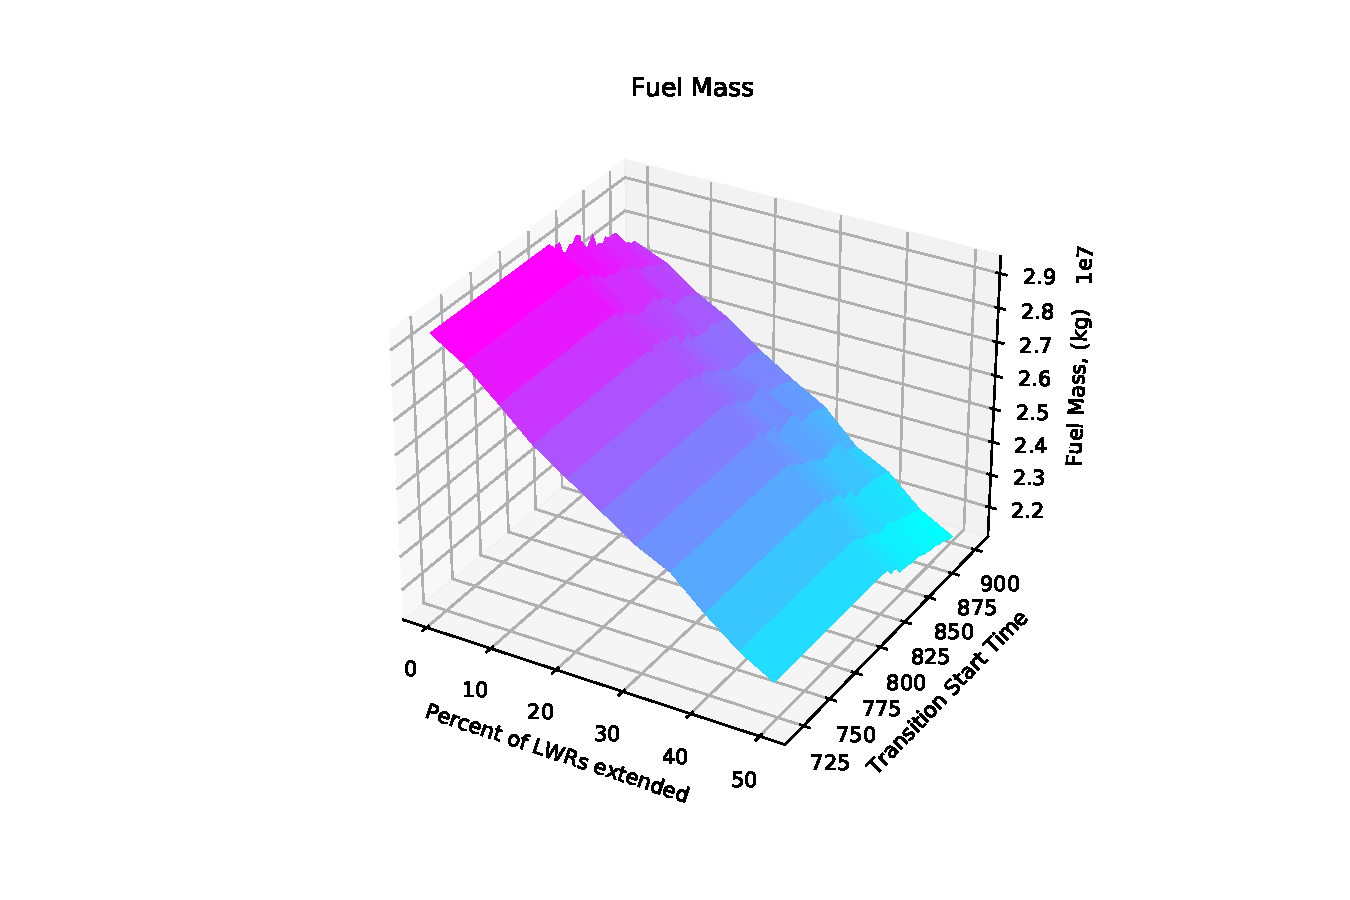
\includegraphics[width=\textwidth, trim=120 0 120 30, clip]{ts_lwr_enr_u.pdf}
        \caption{Effect on total fuel mass.}
        \label{fig:ts_lwr_enr_u}
    \end{subfigure}
    \hfill
    \begin{subfigure}[t]{0.48\textwidth}
        \centering
        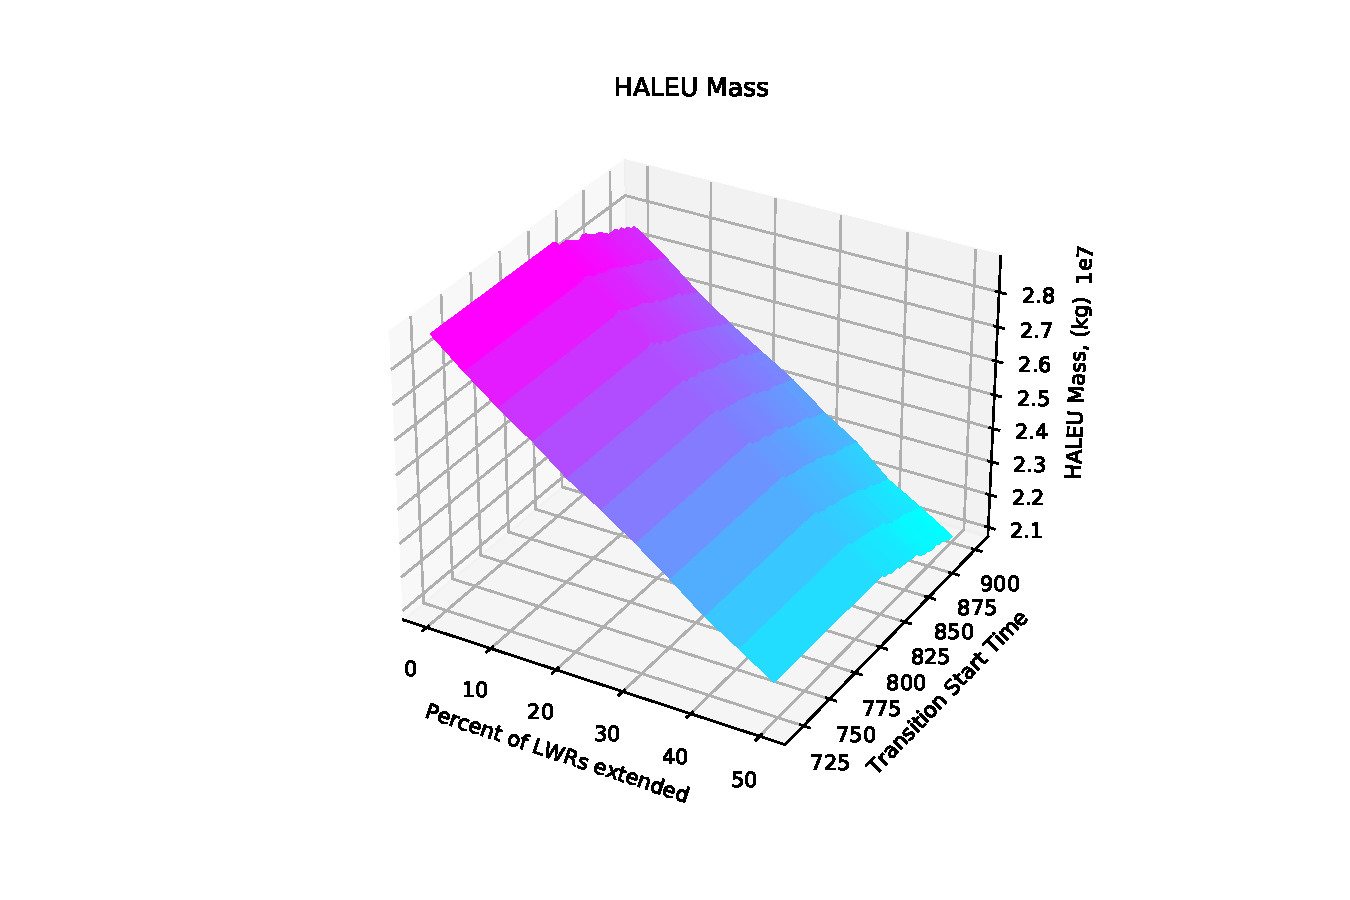
\includegraphics[width=\textwidth, trim=120 0 120 30, clip]{ts_lwr_haleu.pdf}
        \caption{Effect on HALEU mass.}
        \label{fig:ts_lwr_haleu}
    \end{subfigure}
    
    \begin{subfigure}[t]{0.48\textwidth}
        \centering
        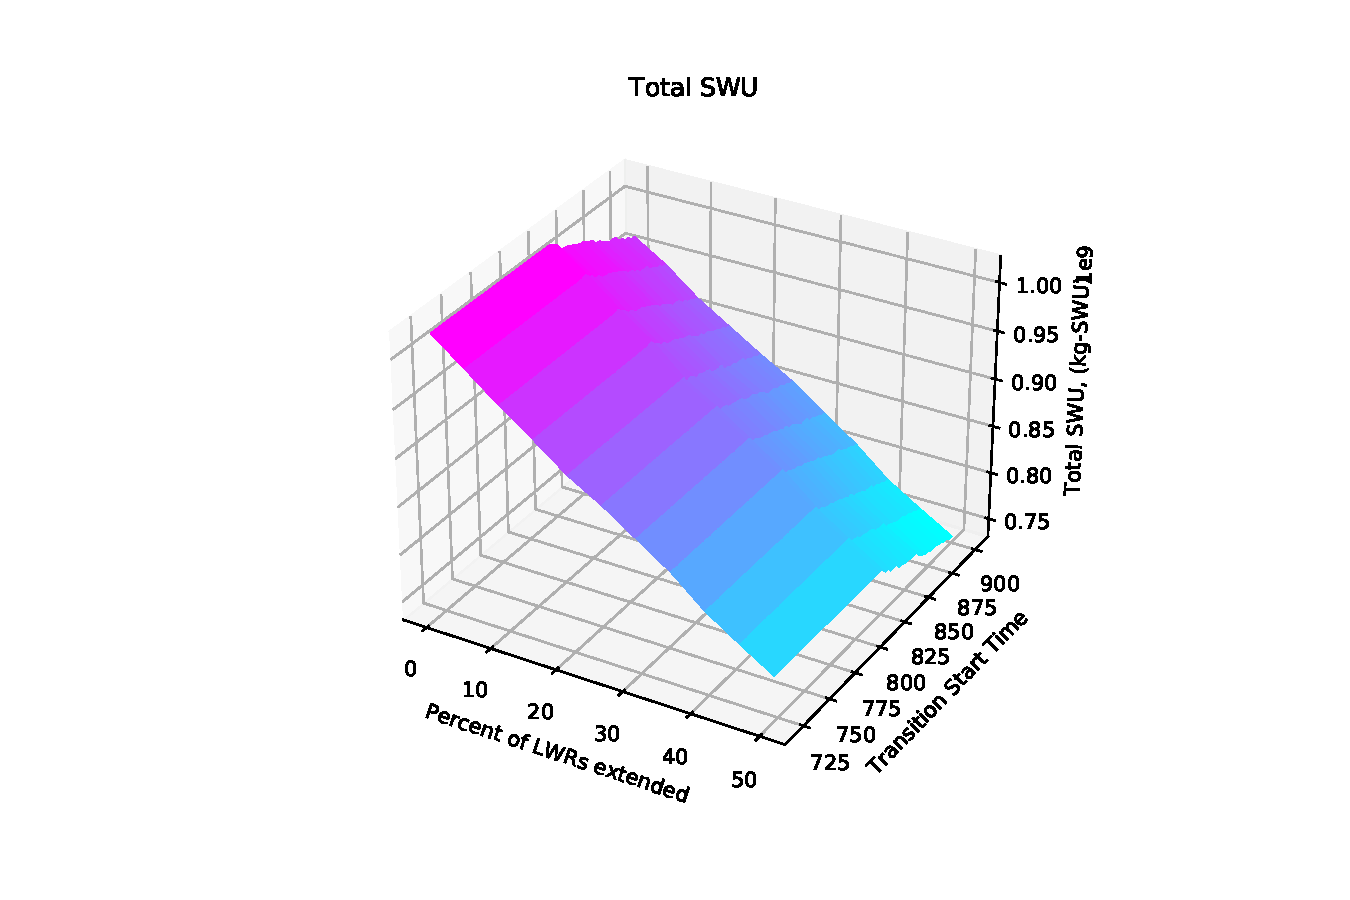
\includegraphics[width=\textwidth, trim=120 0 120 30, clip]{ts_lwr_swu.pdf}
        \caption{Effect on total SWU capacity.}
        \label{fig:ts_lwr_swu}
    \end{subfigure}
    \hfill
    \begin{subfigure}[t]{0.48\textwidth}
        \centering
        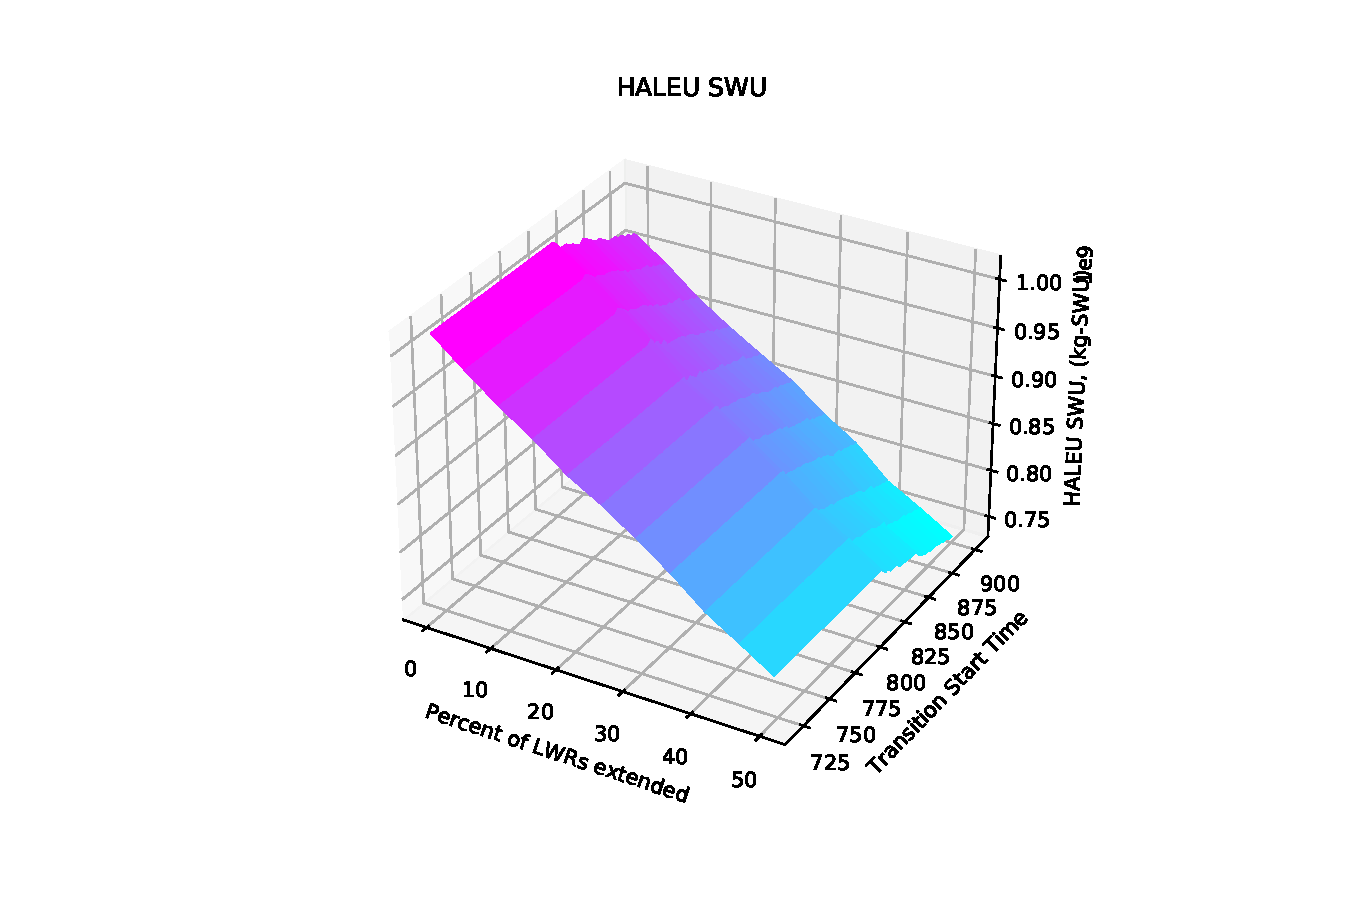
\includegraphics[width=\textwidth, trim=120 0 120 30, clip]{ts_lwr_haleu_swu.pdf}
        \caption{Effect on HALEU SWU capacity.}
        \label{fig:ts_lwr_haleu_swu}
    \end{subfigure}
\end{figure}

\begin{figure}
    \ContinuedFloat    
    \begin{subfigure}[t]{0.48\textwidth}
        \centering
        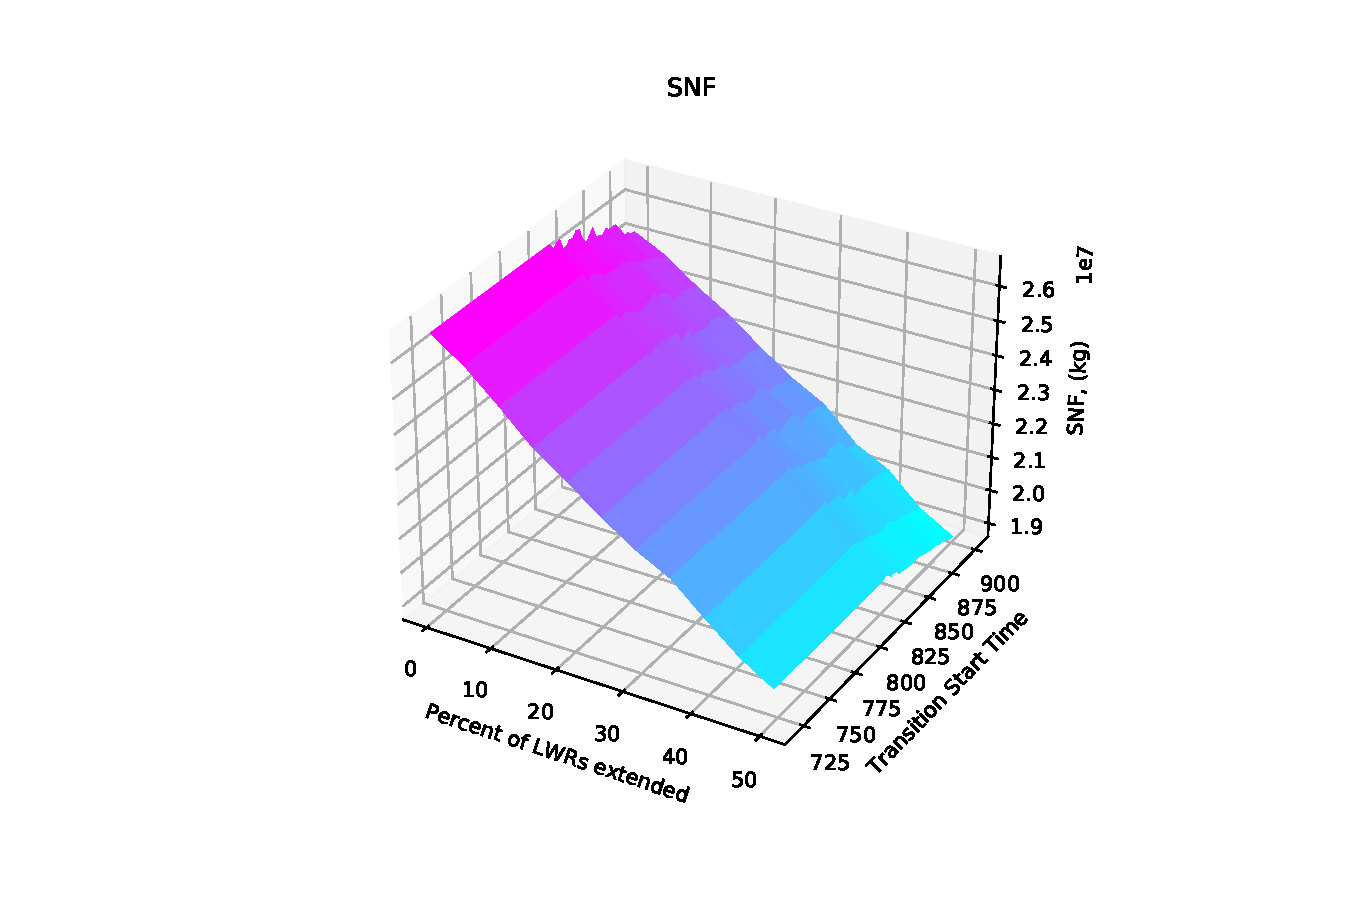
\includegraphics[width=\textwidth, trim=120 0 120 30, clip]{ts_lwr_waste.pdf}
        \caption{Effect on waste mass discharged.}
        \label{fig:ts_lwr_waste}
    \end{subfigure}
    \hfill
    \begin{subfigure}[t]{0.48\textwidth}
        \centering
        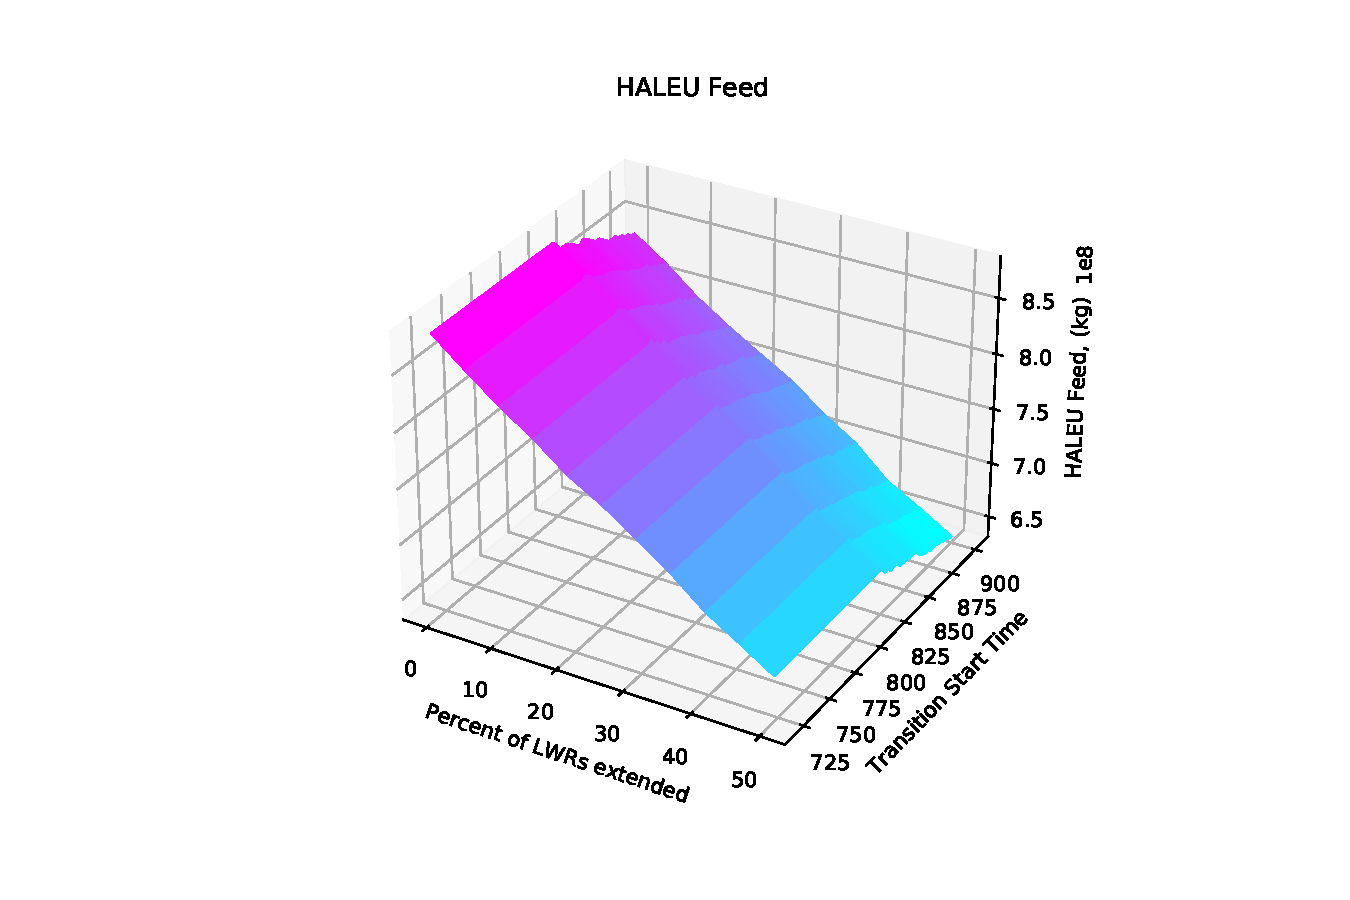
\includegraphics[width=\textwidth, trim=120 0 120 30, clip]{ts_lwr_feed.pdf}
        \caption{Effect on HALEU feed.}
        \label{fig:ts_lwr_feed}
    \end{subfigure}
    \caption{Change in metrics resulting from variations in the 
    transition start time and LWR lifetimes.}
    \label{fig:ts_lwr}
\end{figure}

Figure \ref{fig:ts_xe100_share} shows the results of varying the 
transition start time and Xe-100 build share on the \gls{HALEU} mass, 
\gls{SWU} to produce \gls{HALEU}, waste mass discharged, and feed 
to produce \gls{HALEU}. This figure shows that increasing the 
Xe-100 build share has a greater impact on the metrics than 
changing the transition start time, which is consistent with the 
\gls{OAT} results. There is no clear combined effect from varying these 
parameters together. 

\begin{figure}
    \begin{subfigure}[t]{0.48\textwidth}
        \centering
        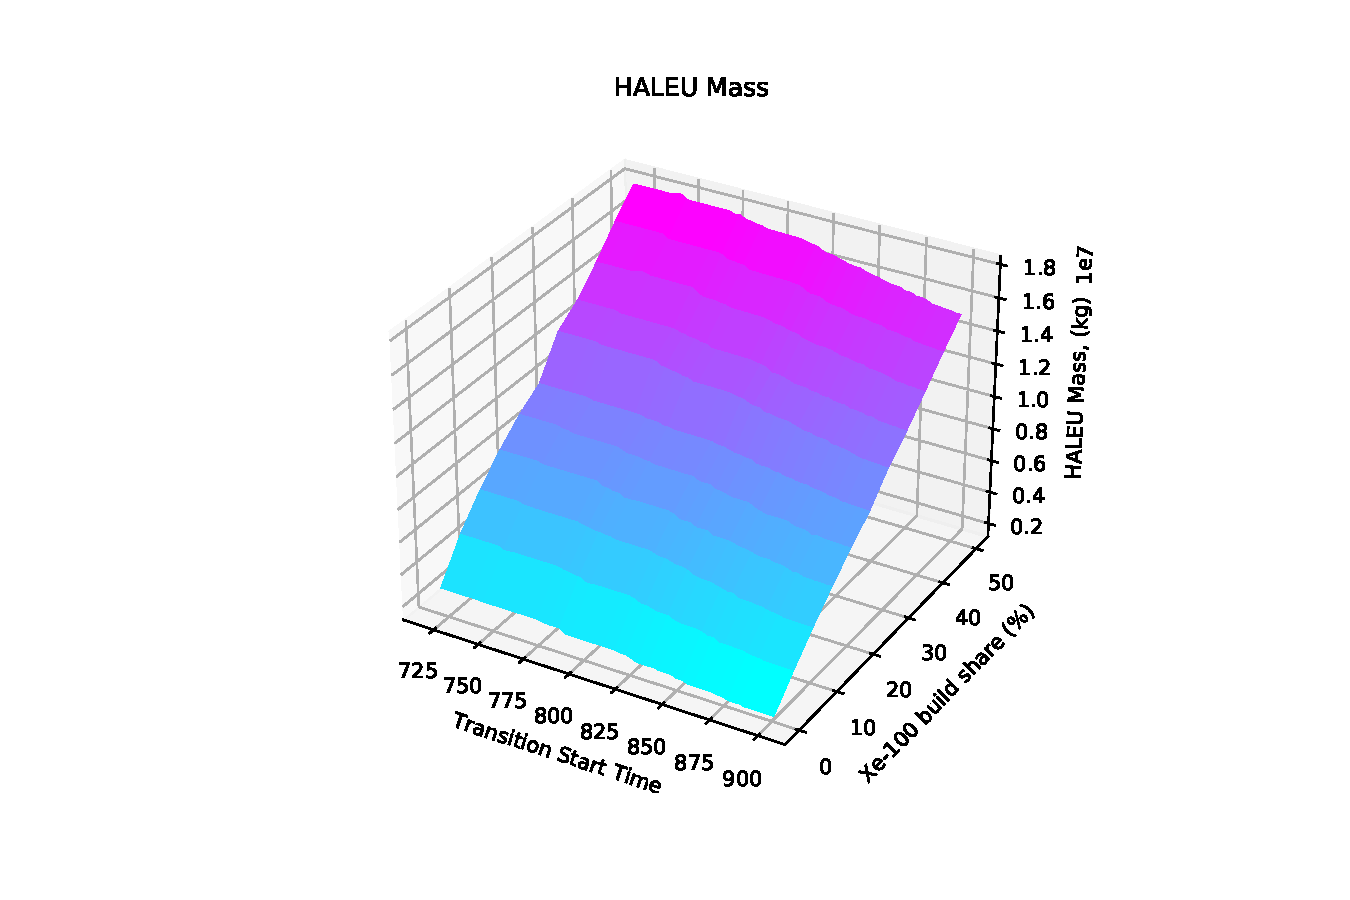
\includegraphics[width=\textwidth, trim=120 0 120 30, clip]{ts_xe100_share_haleu.pdf}
        \caption{Effect on HALEU mass.}
        \label{fig:ts_xe100_share_haleu}
    \end{subfigure}
    \begin{subfigure}[t]{0.48\textwidth}
        \centering
        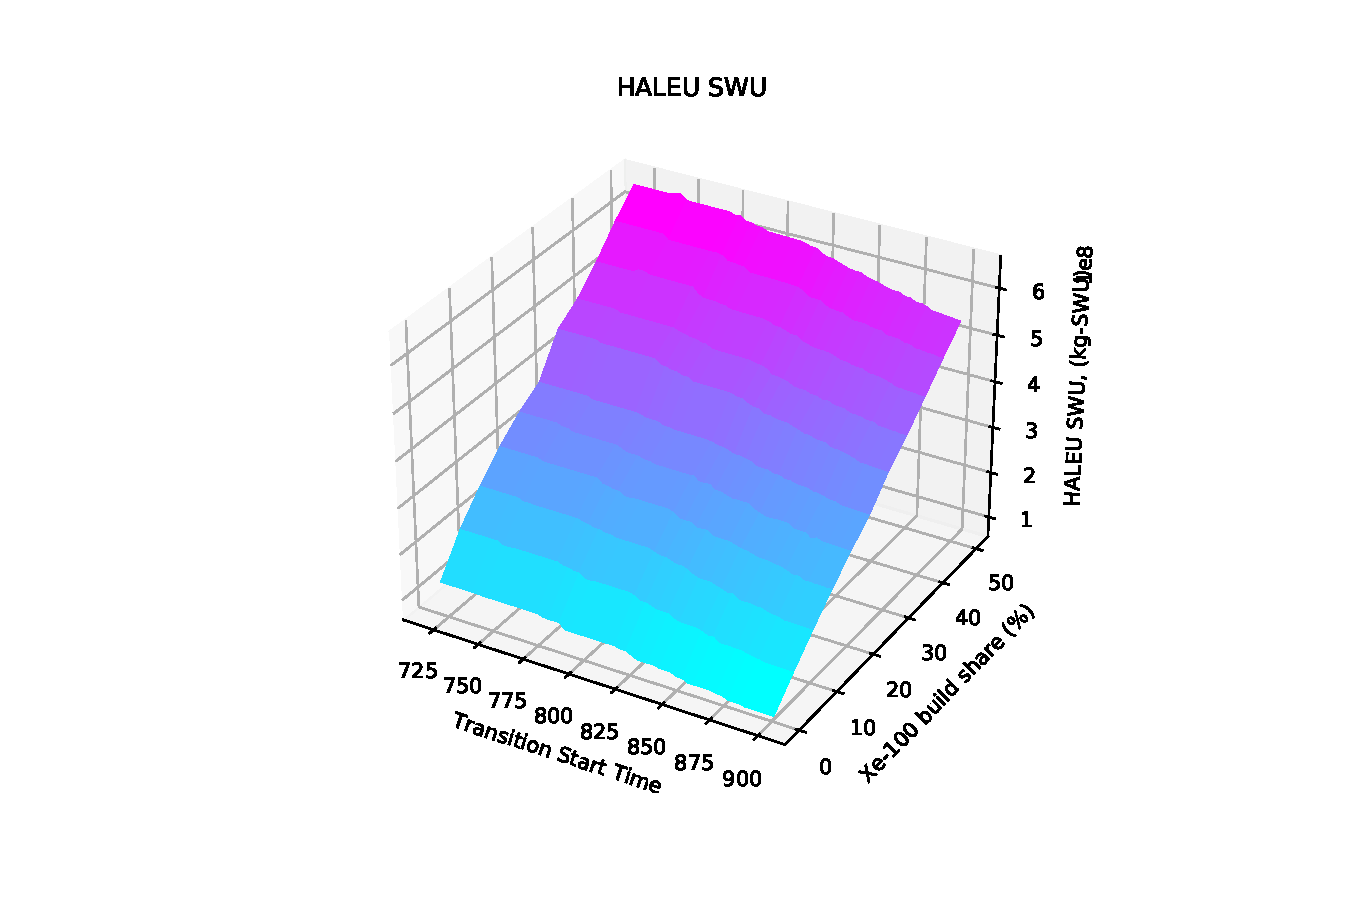
\includegraphics[width=\textwidth, trim=120 0 120 30, clip]{ts_xe100_share_haleu_swu.pdf}
        \caption{Effect on HALEU SWU capacity.}
        \label{fig:ts_xe100_share_haleu_swu}
    \end{subfigure}
    
    \begin{subfigure}[t]{0.48\textwidth}
        \centering
        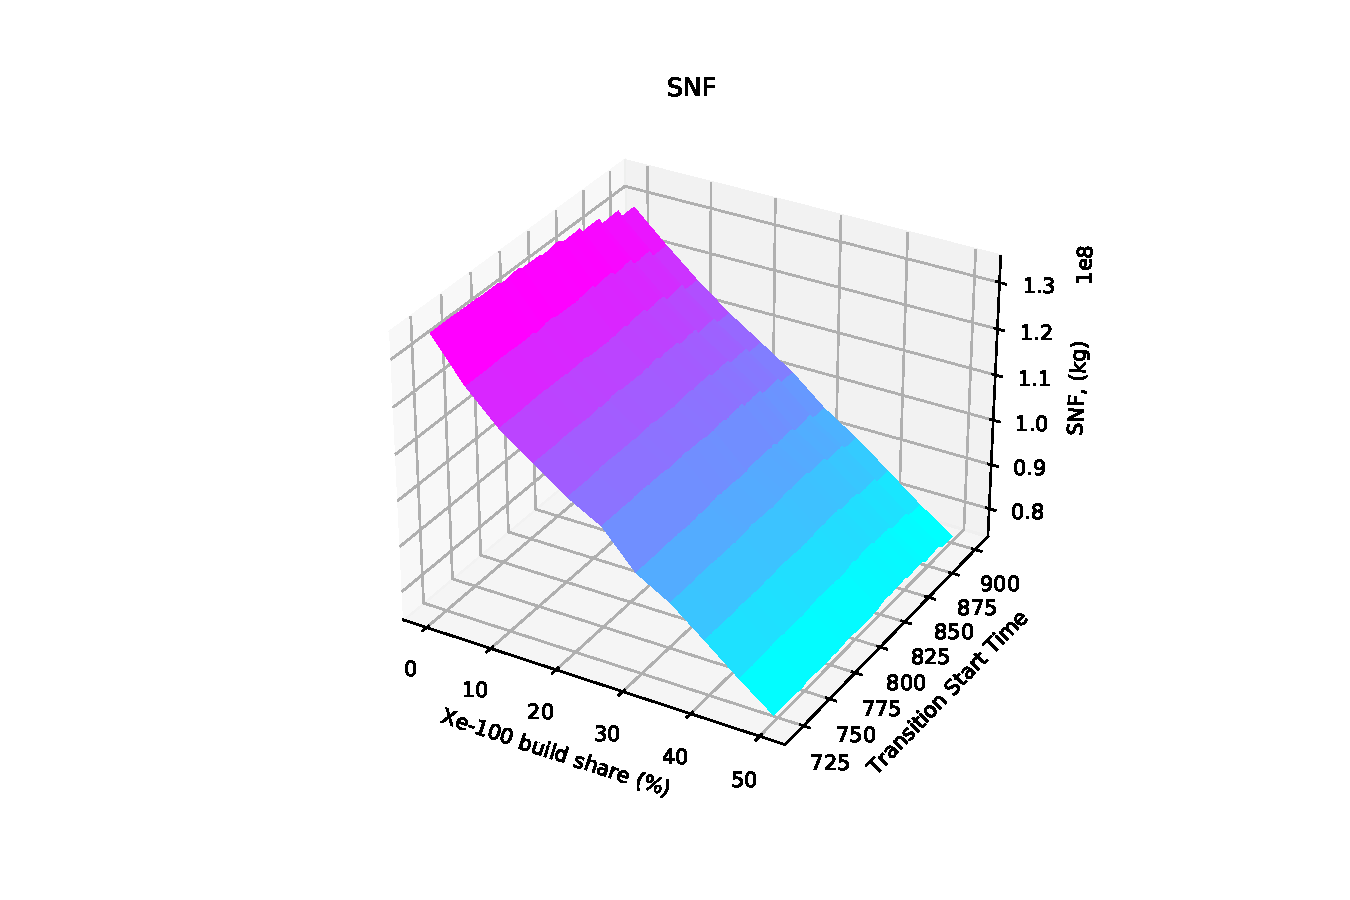
\includegraphics[width=\textwidth, trim=120 0 120 30, clip]{ts_xe100_share_waste.pdf}
        \caption{Effect on waste mass discharged.}
        \label{fig:ts_xe100_share_waste}
    \end{subfigure}
    \hfill
    \begin{subfigure}[t]{0.48\textwidth}
        \centering
        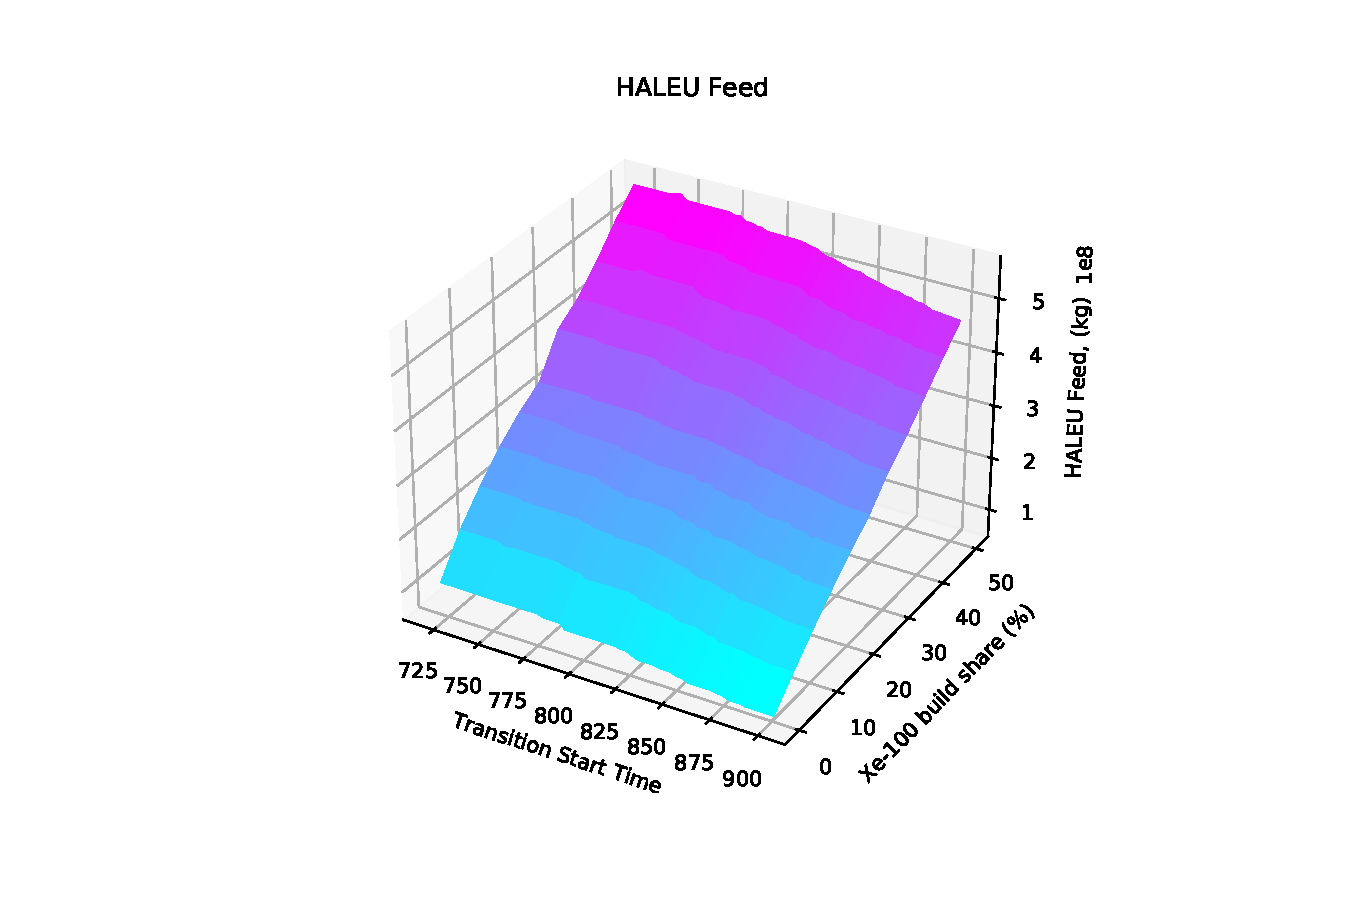
\includegraphics[width=\textwidth, trim=120 0 120 30, clip]{ts_xe100_share_feed.pdf}
        \caption{Effect on HALEU feed.}
        \label{fig:ts_xe100_share_feed}
    \end{subfigure}
    \caption{Change in metrics resulting from variations in the 
    transition start time and Xe-100 build share.}
    \label{fig:ts_xe100_share}
\end{figure}

Figure \ref{fig:ts_mmr_share} shows the results of varying the 
transition start time and the \gls{MMR} build share on all 
six of the metrics. 

\begin{figure}
    \begin{subfigure}[t]{0.48\textwidth}
        \centering
        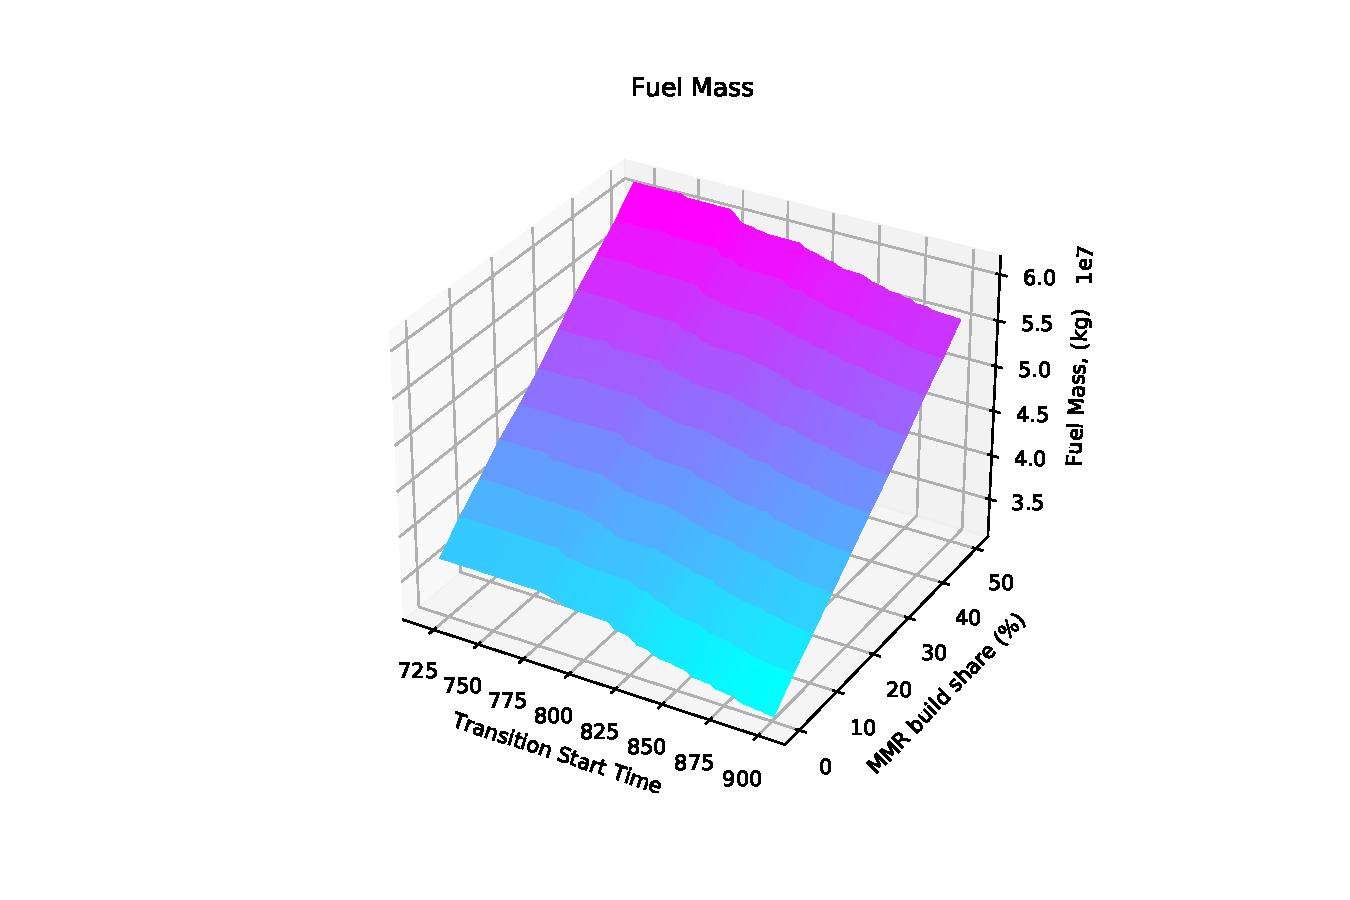
\includegraphics[width=\textwidth, trim=120 0 120 30, clip]{ts_mmr_share_enr_u.pdf}
        \caption{Effect on total fuel mass.}
        \label{fig:ts_mmr_share_enr_u}
    \end{subfigure}
    \hfill
    \begin{subfigure}[t]{0.48\textwidth}
        \centering
        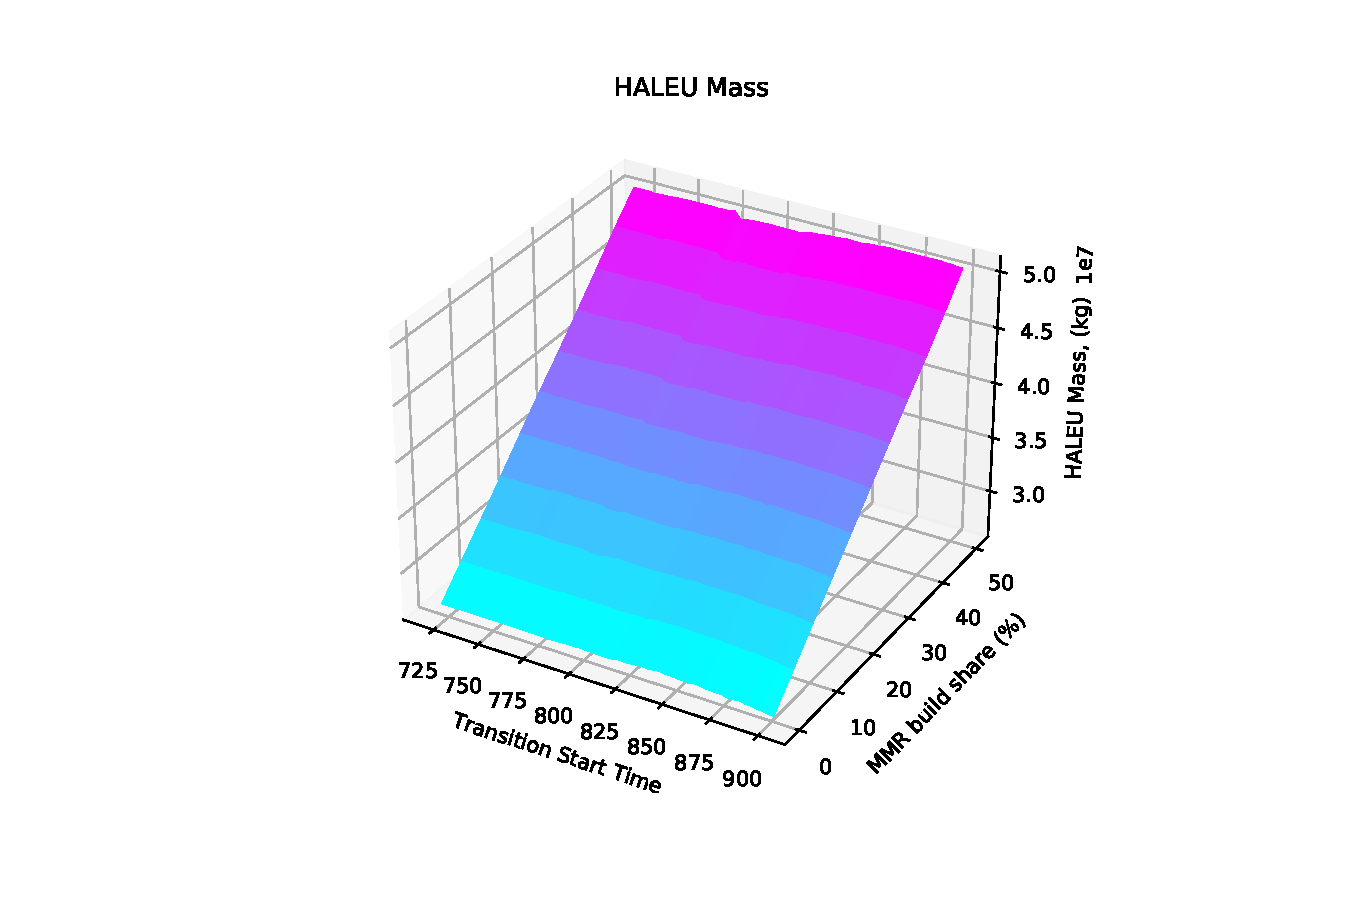
\includegraphics[width=\textwidth, trim=120 0 120 30, clip]{ts_mmr_share_haleu.pdf}
        \caption{Effect on HALEU mass.}
        \label{fig:ts_mmr_share_haleu}
    \end{subfigure}
    
    \begin{subfigure}[t]{0.48\textwidth}
        \centering
        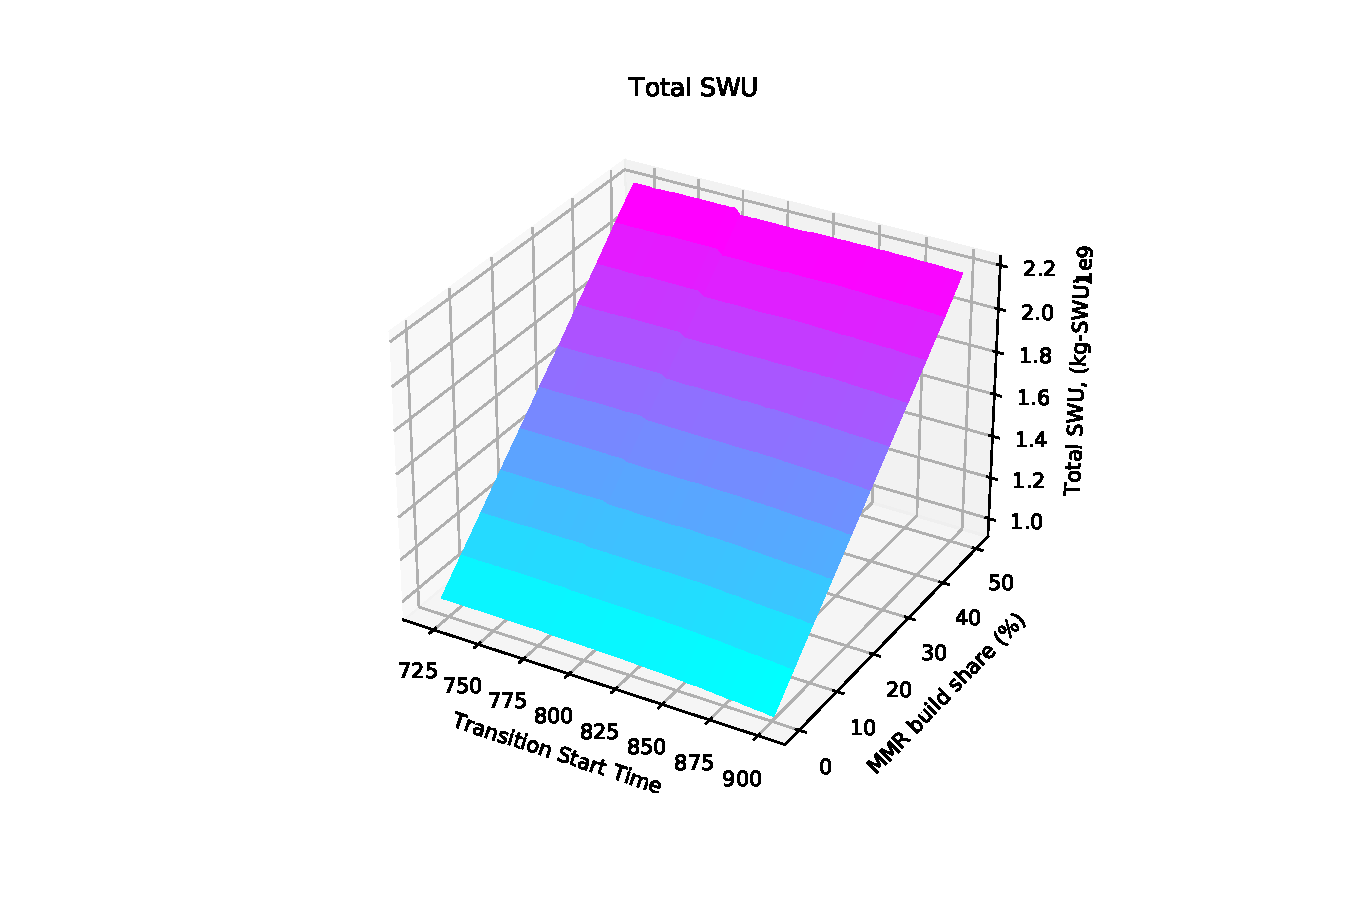
\includegraphics[width=\textwidth, trim=120 0 120 30, clip]{ts_mmr_share_swu.pdf}
        \caption{Effect on total SWU capacity.}
        \label{fig:ts_mmr_share_swu}
    \end{subfigure}
    \hfill
    \begin{subfigure}[t]{0.48\textwidth}
        \centering
        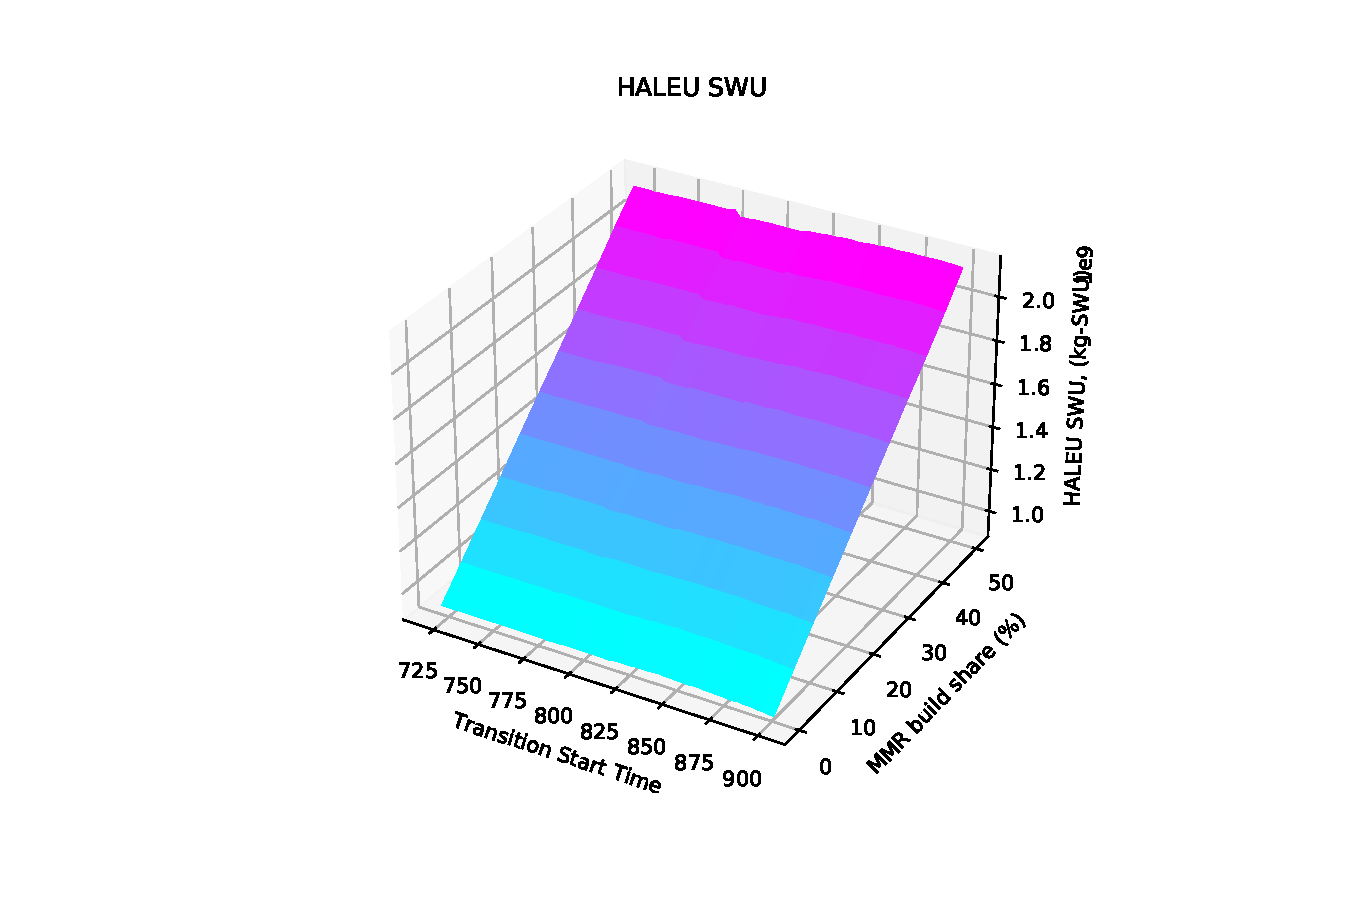
\includegraphics[width=\textwidth, trim=120 0 120 30, clip]{ts_mmr_share_haleu_swu.pdf}
        \caption{Effect on HALEU SWU capacity.}
        \label{fig:ts_mmr_share_haleu_swu}
    \end{subfigure}
\end{figure}

\begin{figure}
    \ContinuedFloat
    \begin{subfigure}[t]{0.48\textwidth}
        \centering
        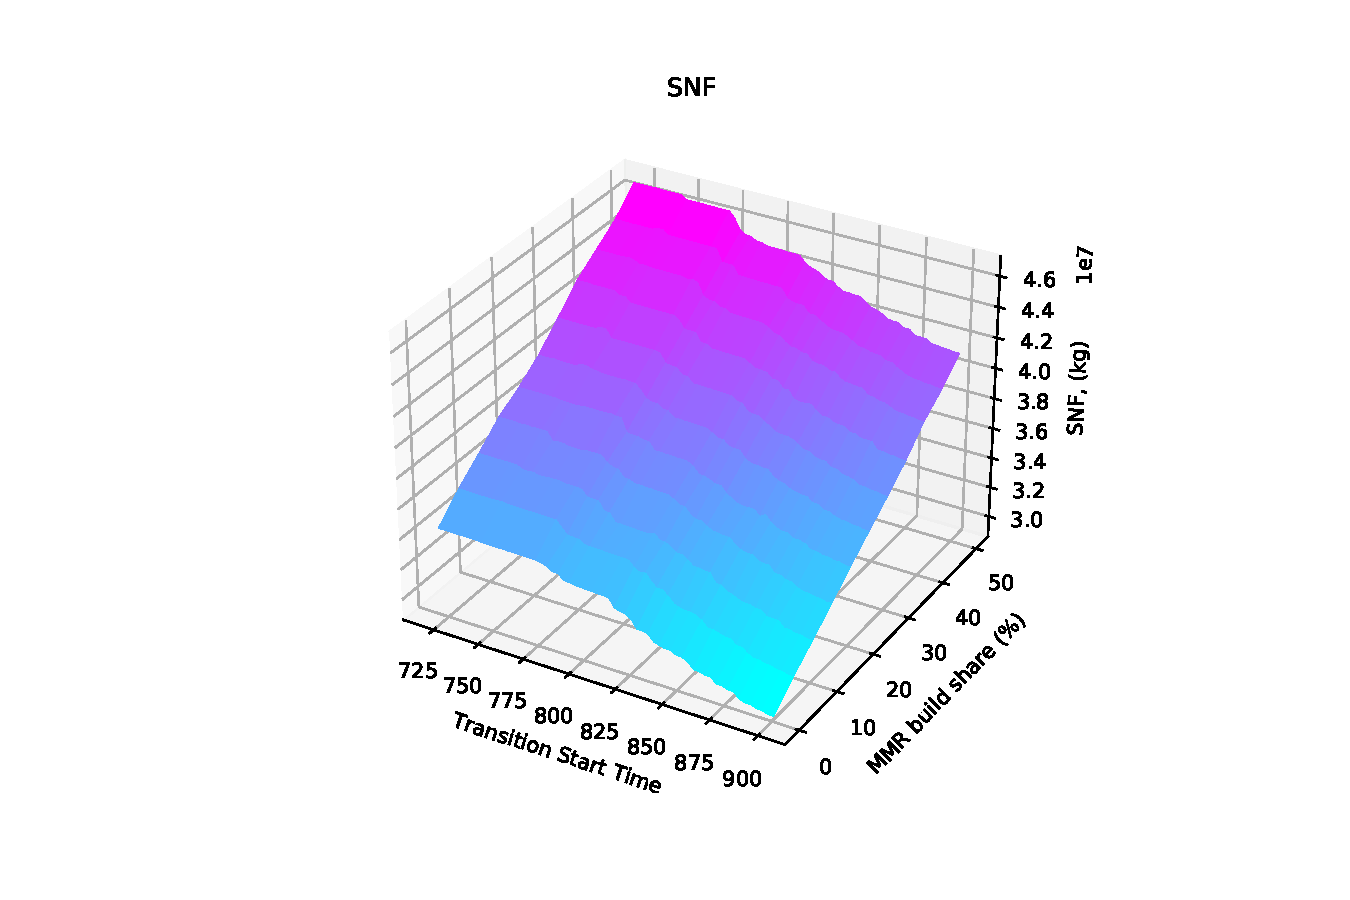
\includegraphics[width=\textwidth, trim=120 0 120 30, clip]{ts_mmr_share_waste.pdf}
        \caption{Effect on waste mass discharged.}
        \label{fig:ts_mmr_share_waste}
    \end{subfigure}
    \hfill
    \begin{subfigure}[t]{0.48\textwidth}
        \centering
        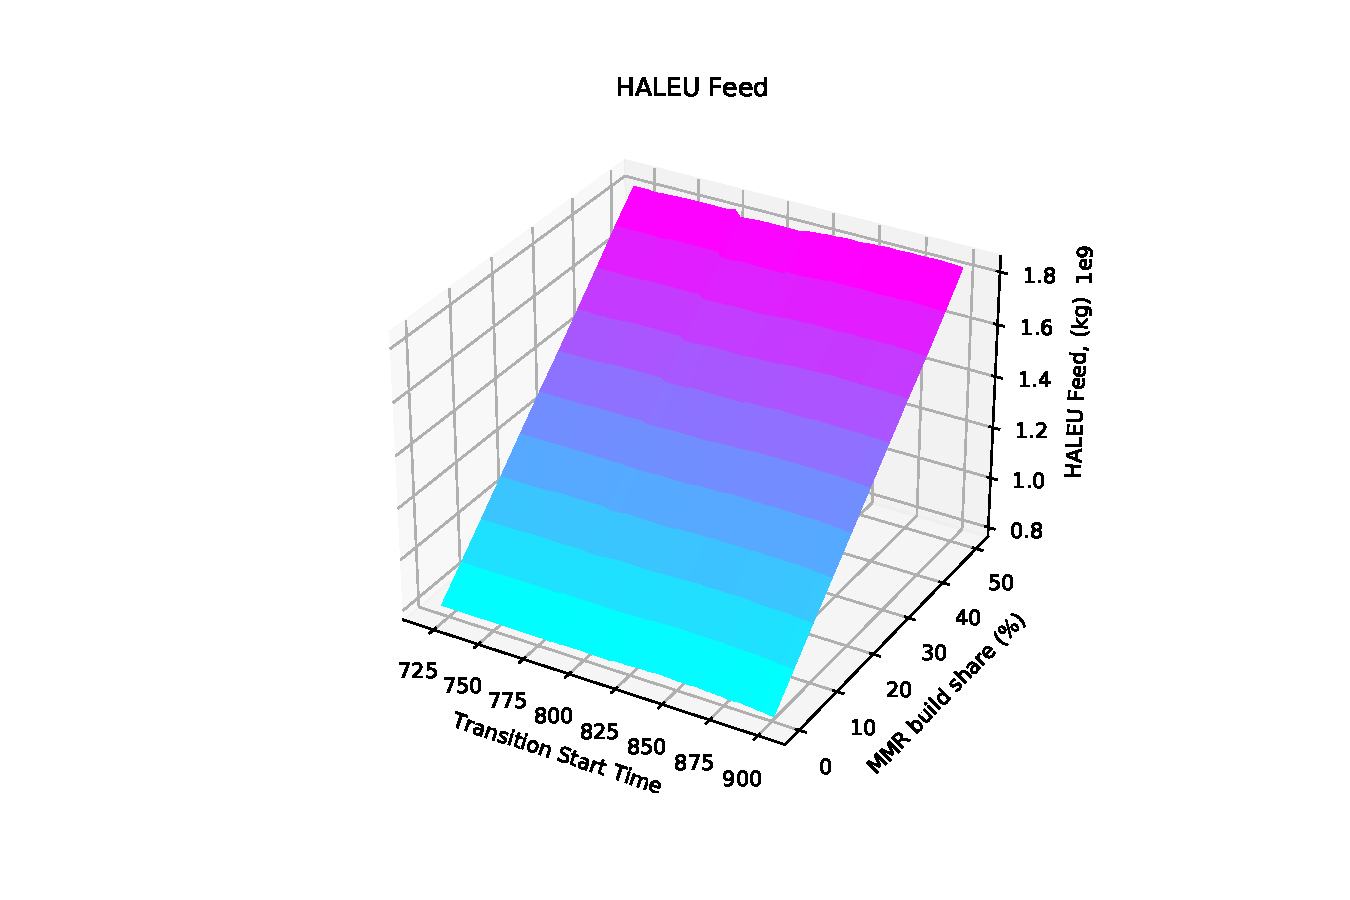
\includegraphics[width=\textwidth, trim=120 0 120 30, clip]{ts_mmr_share_feed.pdf}
        \caption{Effect on HALEU feed.}
        \label{fig:ts_mmr_share_feed}
    \end{subfigure}
    \caption{Change in metrics resulting from variations in the 
    transition start time and MMR build share.}
    \label{fig:ts_mmr_share}
\end{figure}

Figure \ref{fig:ts_voygr_share} shows the effects of varying the 
transition start time and the VOYGR build share on all six of the 
metrics. 

\begin{figure}
    \begin{subfigure}[t]{0.48\textwidth}
        \centering
        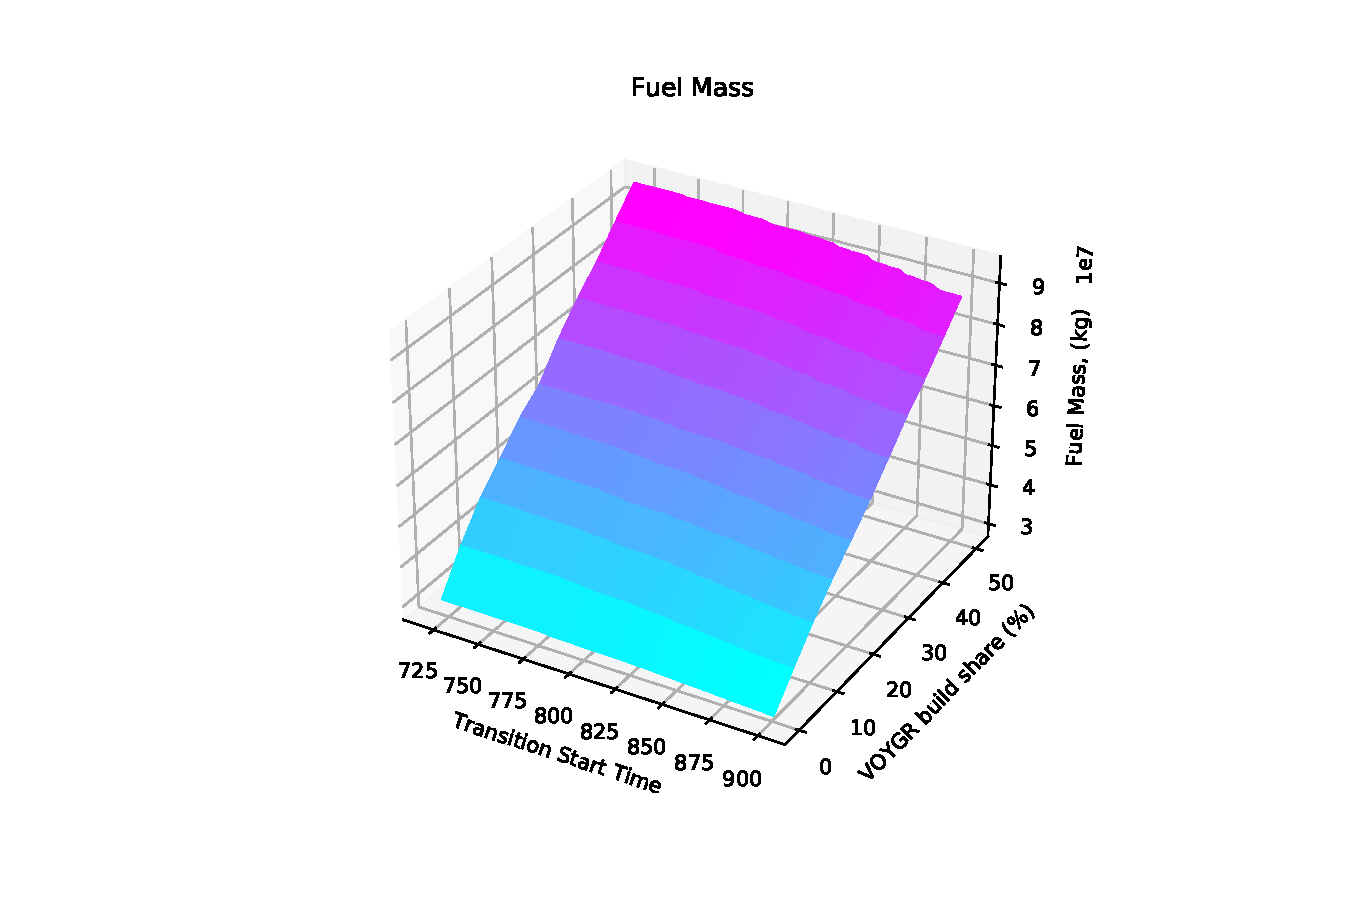
\includegraphics[width=\textwidth, trim=120 0 120 30, clip]{ts_voygr_share_enr_u.pdf}
        \caption{Effect on total fuel mass.}
        \label{fig:ts_voygr_share_enr_u}
    \end{subfigure}
    \hfill
    \begin{subfigure}[t]{0.48\textwidth}
        \centering
        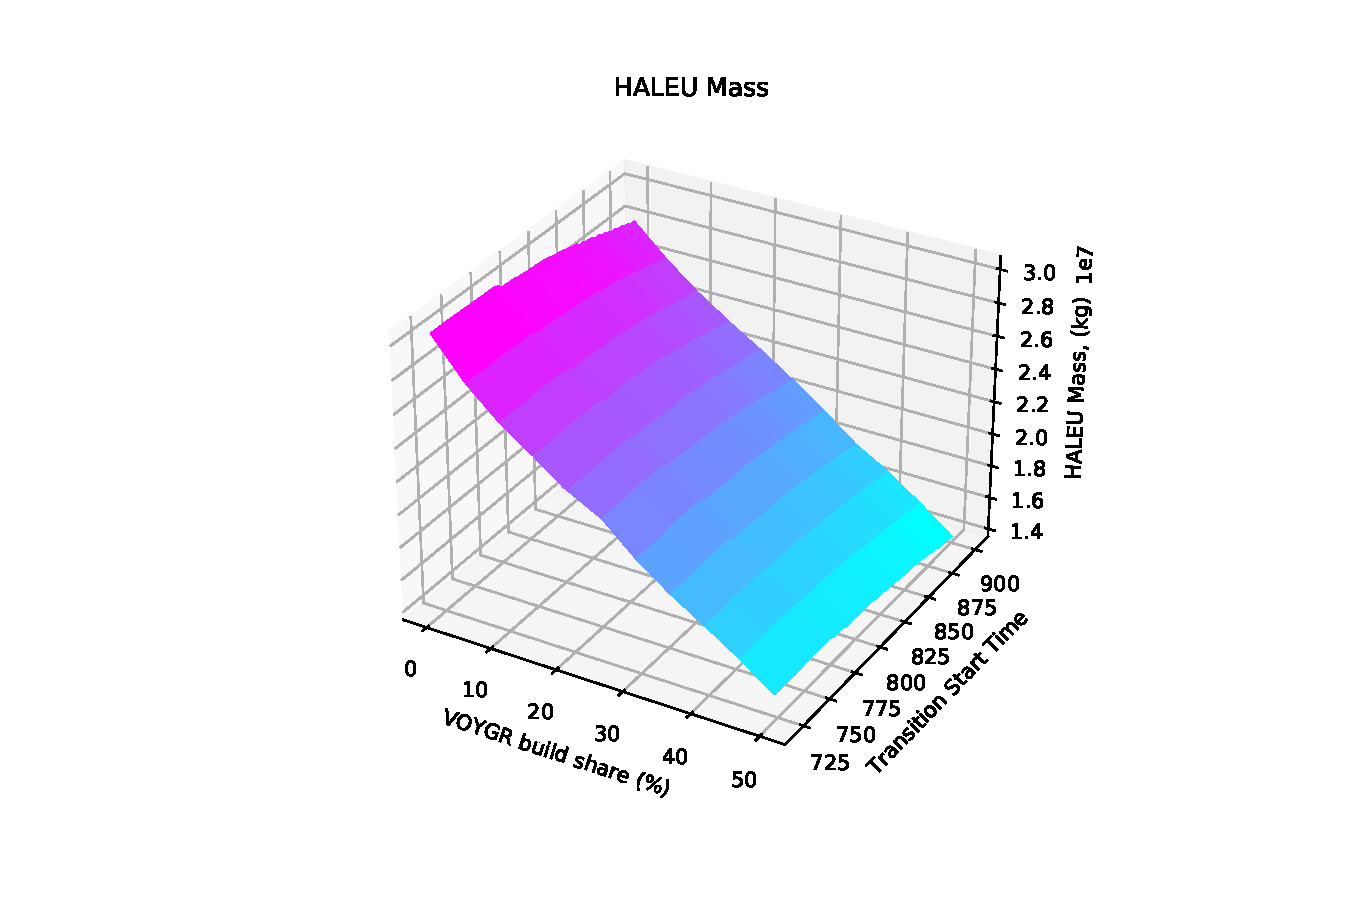
\includegraphics[width=\textwidth, trim=120 0 120 30, clip]{ts_voygr_share_haleu.pdf}
        \caption{Effect on HALEU mass.}
        \label{fig:ts_voygr_share_haleu}
    \end{subfigure}
\end{figure}

\begin{figure}
    \ContinuedFloat
    \begin{subfigure}[t]{0.48\textwidth}
        \centering
        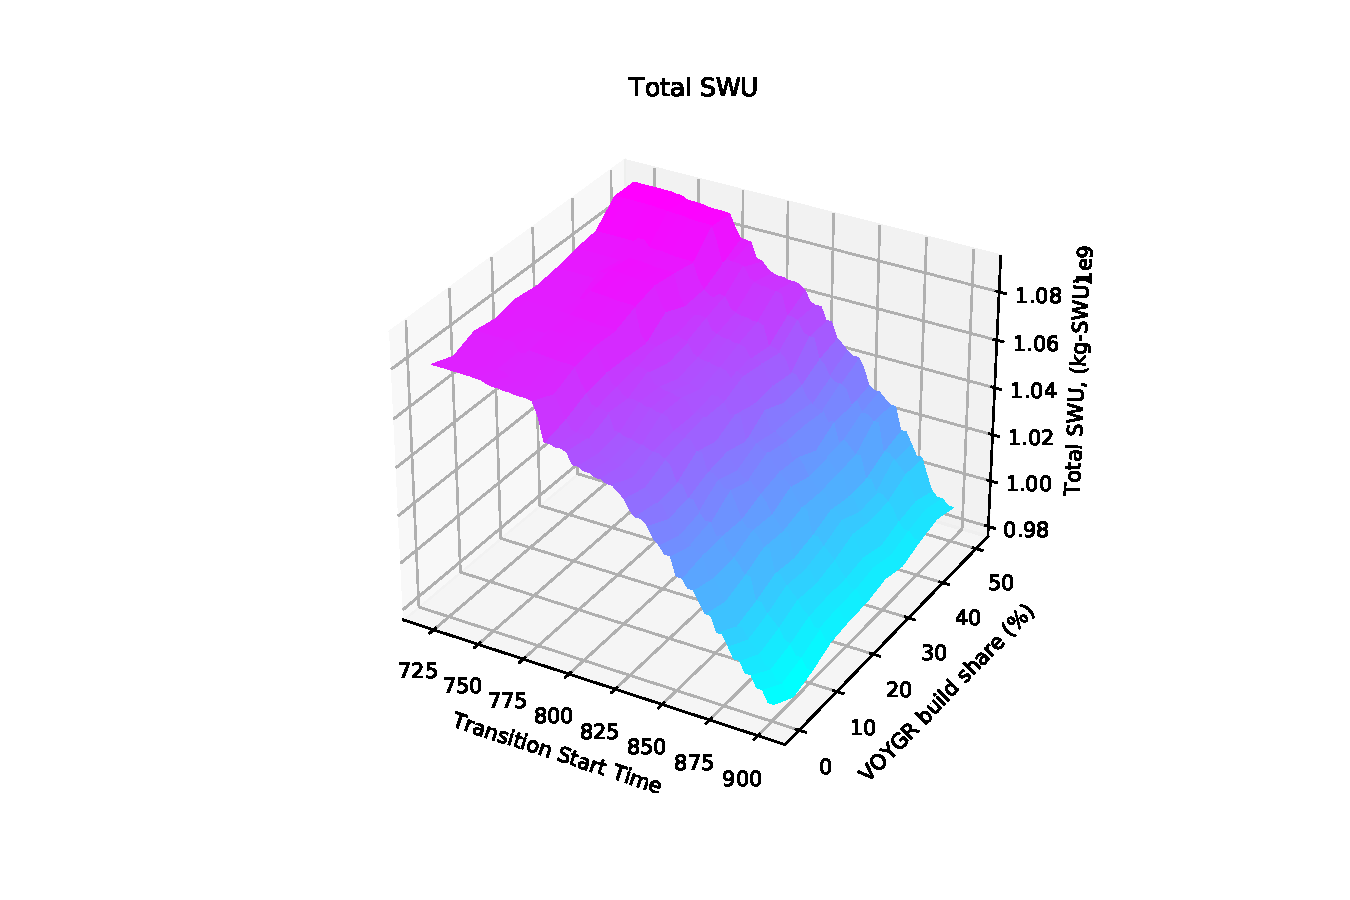
\includegraphics[width=\textwidth, trim=120 0 120 30, clip]{ts_voygr_share_swu.pdf}
        \caption{Effect on total SWU capacity.}
        \label{fig:ts_voygr_share_swu}
    \end{subfigure}
    \hfill
    \begin{subfigure}[t]{0.48\textwidth}
        \centering
        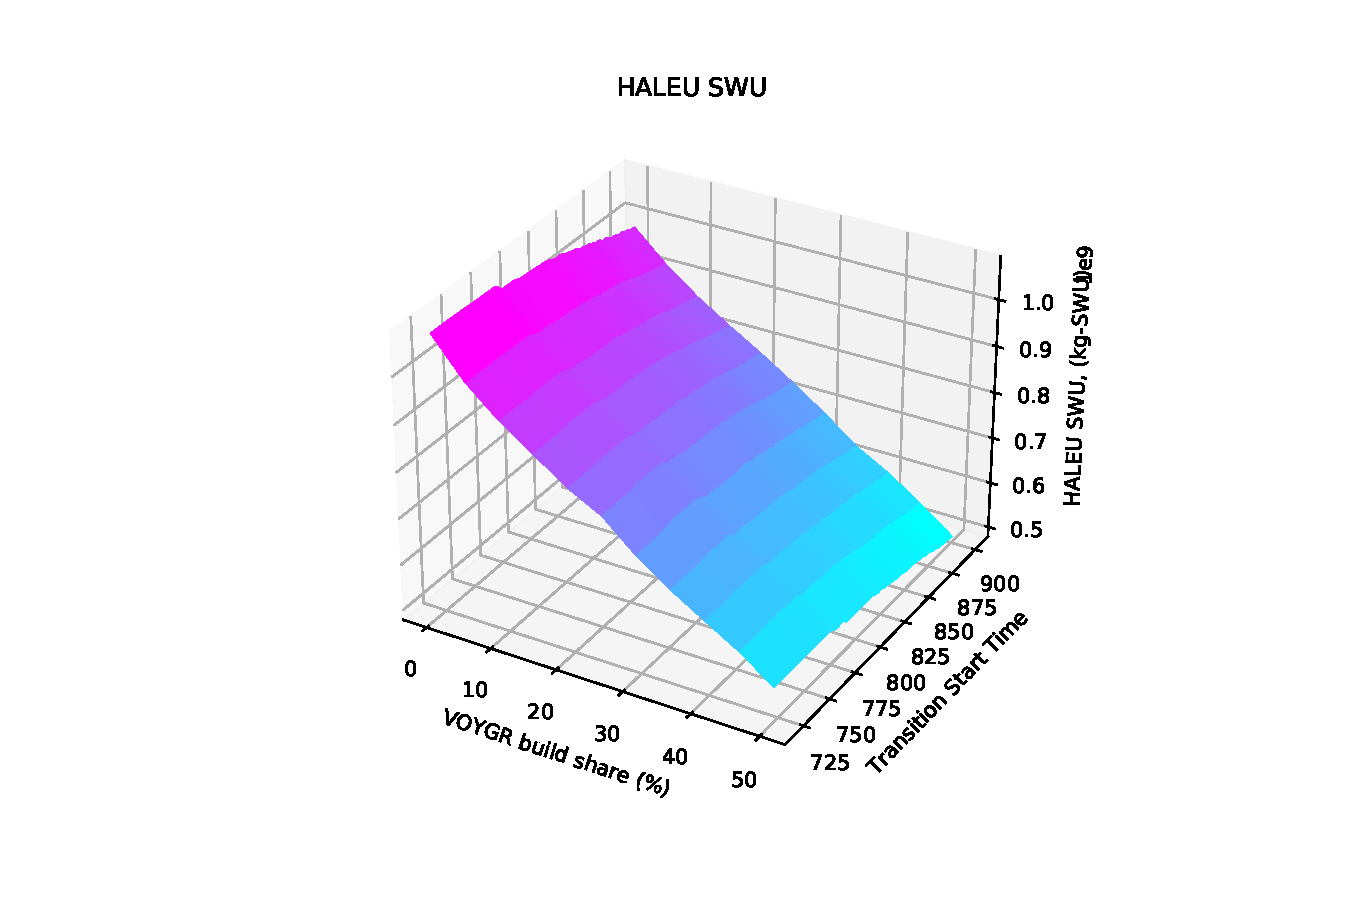
\includegraphics[width=\textwidth, trim=120 0 120 30, clip]{ts_voygr_share_haleu_swu.pdf}
        \caption{Effect on HALEU SWU capacity.}
        \label{fig:ts_voygr_share_haleu_swu}
    \end{subfigure}
    
    \begin{subfigure}[t]{0.48\textwidth}
        \centering
        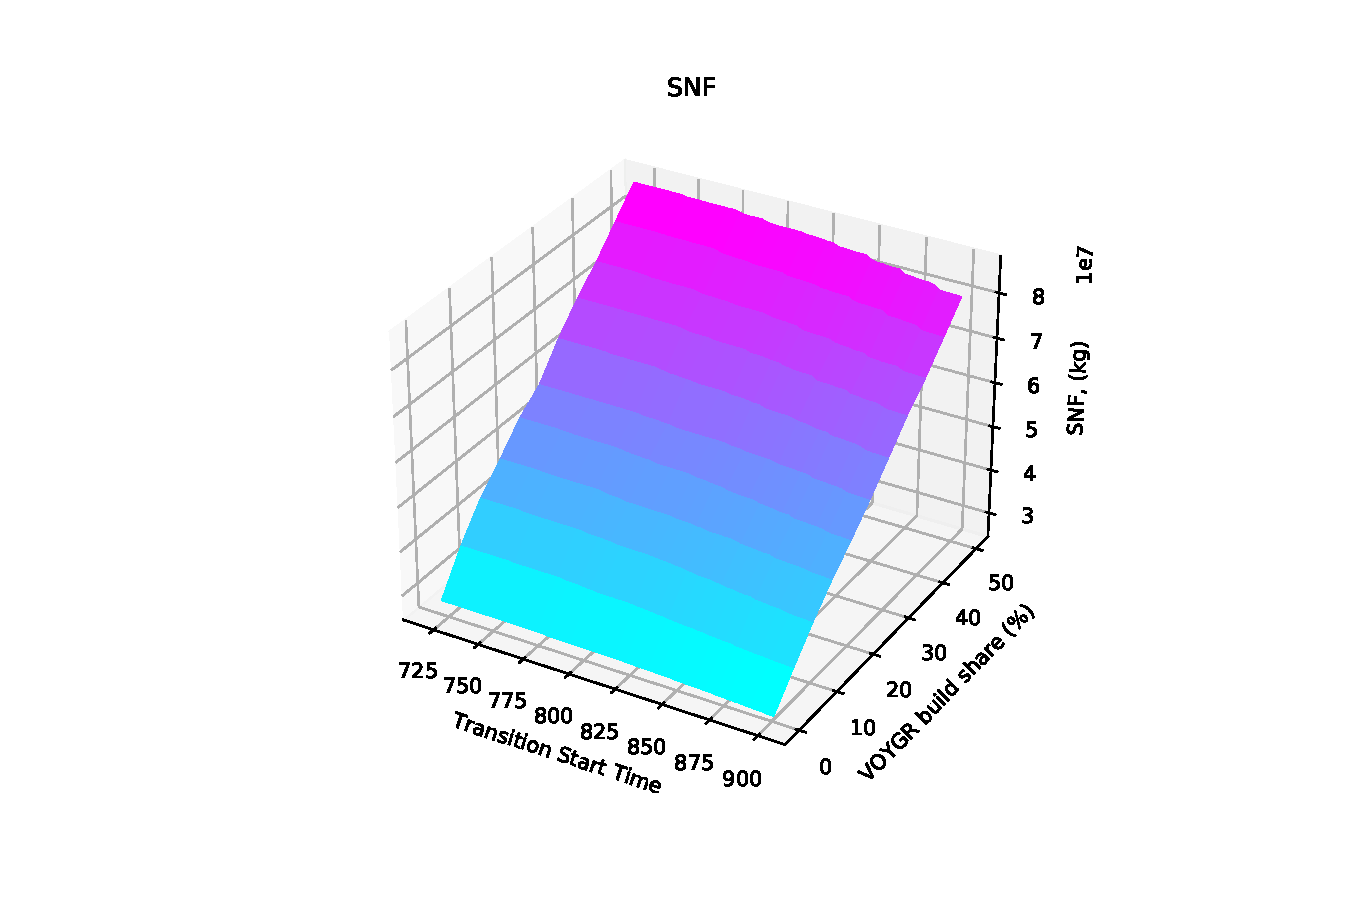
\includegraphics[width=\textwidth, trim=120 0 120 30, clip]{ts_voygr_share_waste.pdf}
        \caption{Effect on waste mass discharged.}
        \label{fig:ts_voygr_share_waste}
    \end{subfigure}
    \hfill
    \begin{subfigure}[t]{0.48\textwidth}
        \centering
        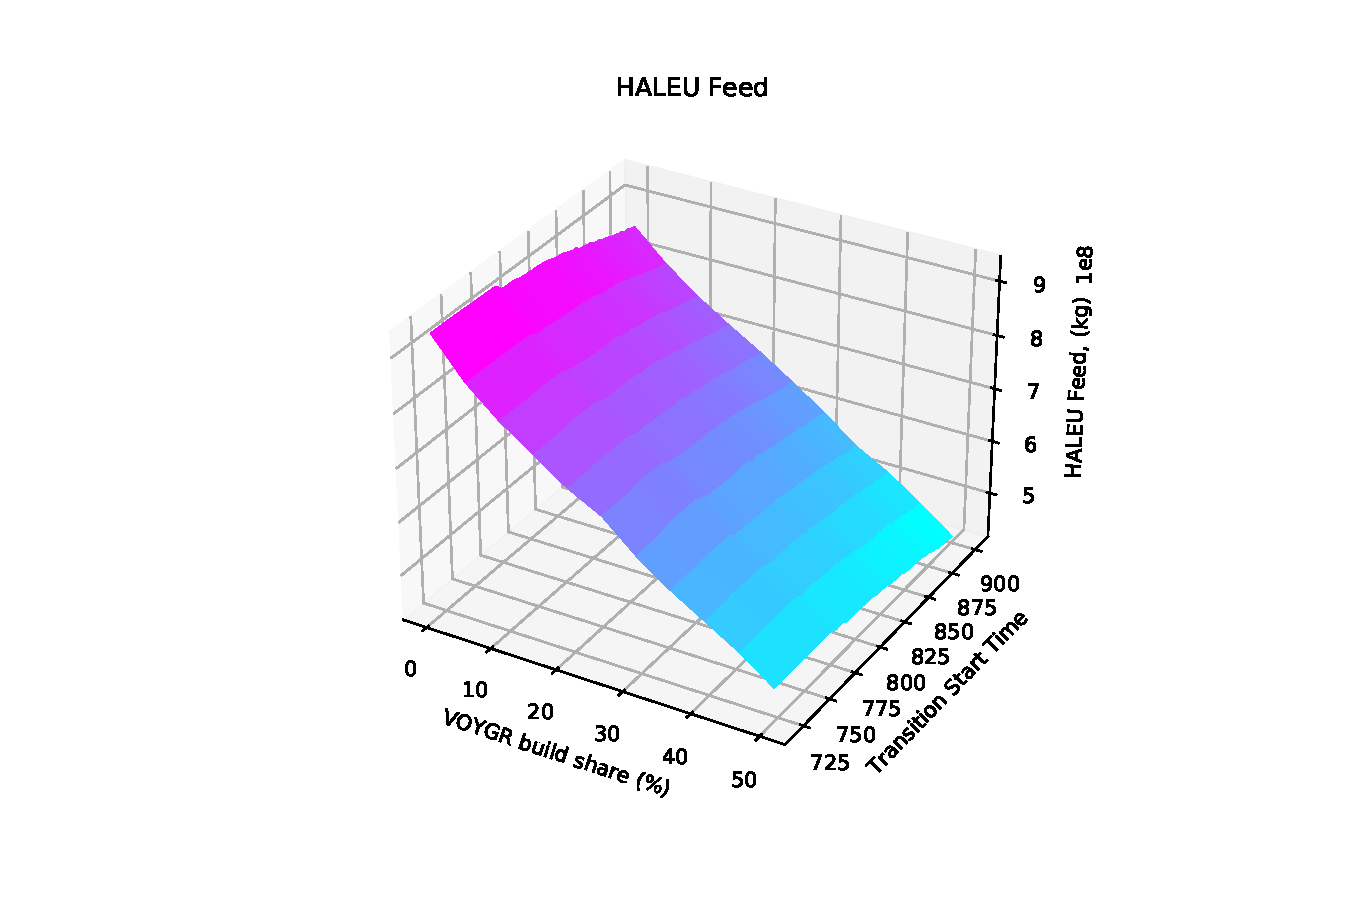
\includegraphics[width=\textwidth, trim=120 0 120 30, clip]{ts_voygr_share_feed.pdf}
        \caption{Effect on HALEU feed.}
        \label{fig:ts_voygr_share_feed}
    \end{subfigure}
    \caption{Change in metrics resulting from variations in the 
    transition start time and VOYGR build share.}
    \label{fig:ts_voygr_share}
\end{figure}

Figure \ref{fig:ts_xe100_bu} shows the effects of varying the 
transition start time and the Xe-100 discharge burnup on all six 
metrics. 
\begin{figure}
    \begin{subfigure}[t]{0.48\textwidth}
        \centering
        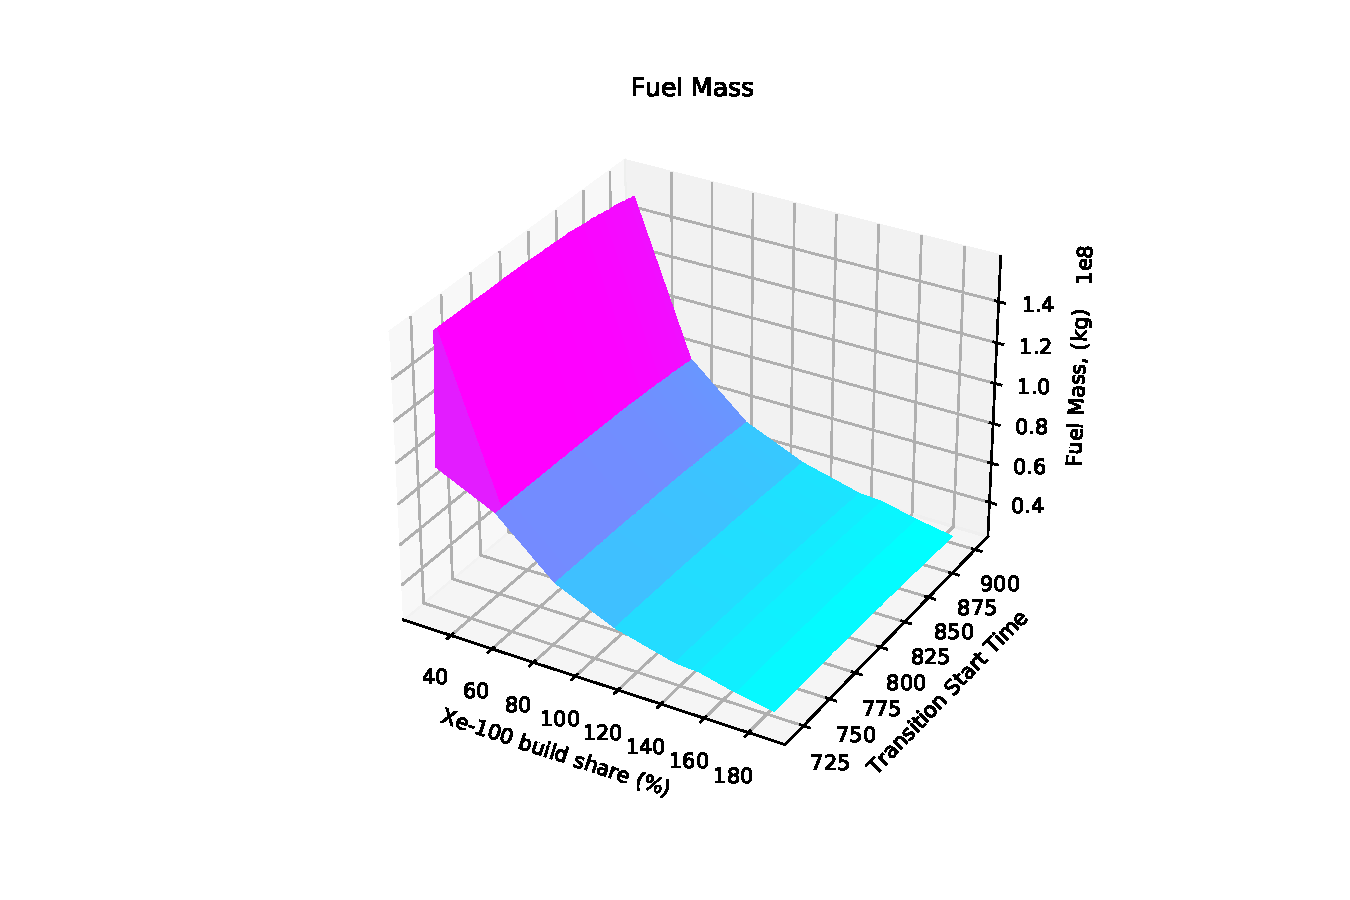
\includegraphics[width=\textwidth, trim=120 0 120 30, clip]{ts_xe100_burnup_enr_u.pdf}
        \caption{Effect on total fuel mass.}
        \label{fig:ts_xe100_bu_enr_u}
    \end{subfigure}
    \hfill
    \begin{subfigure}[t]{0.48\textwidth}
        \centering
        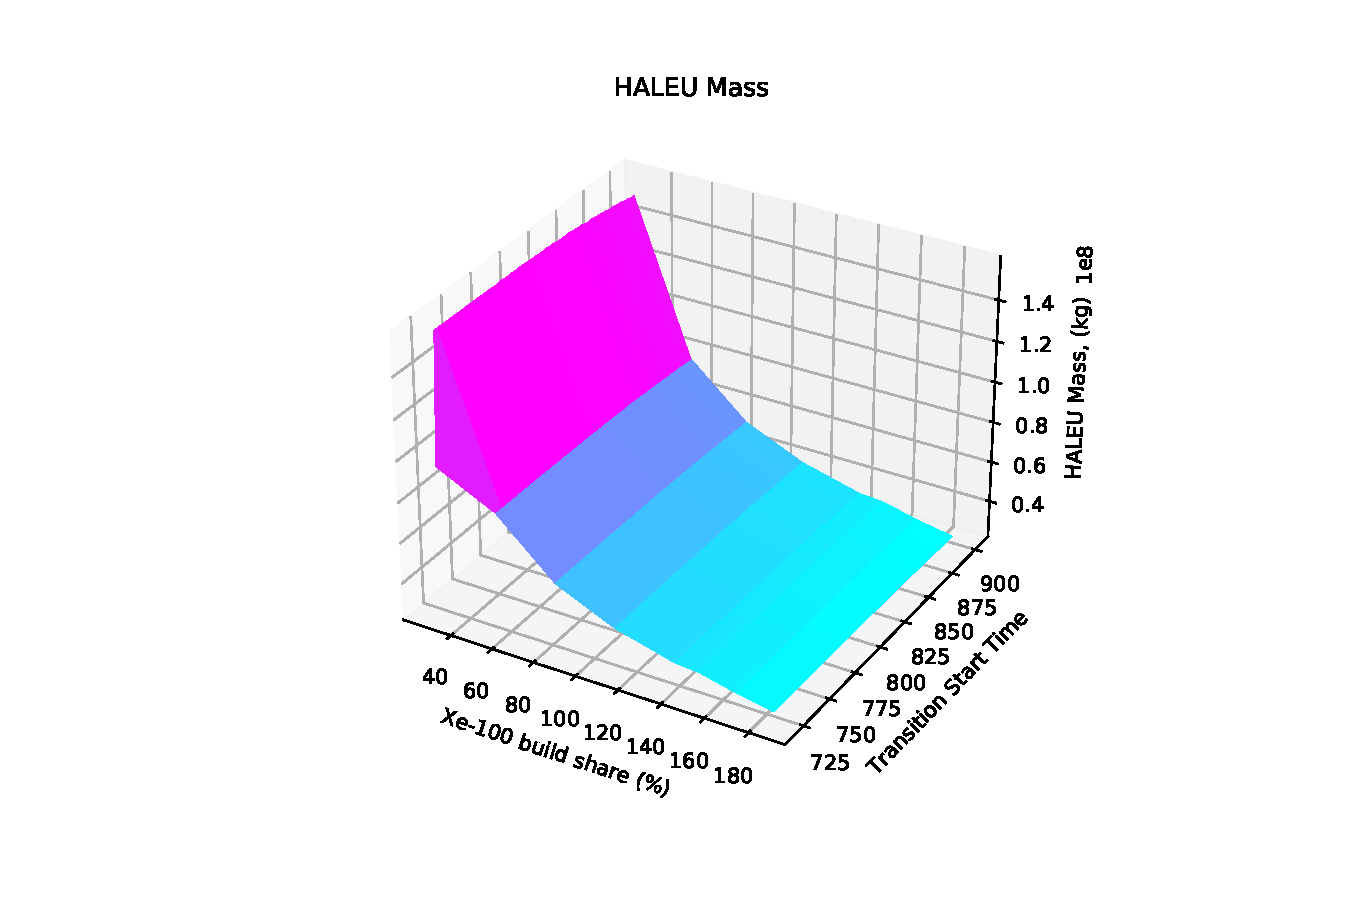
\includegraphics[width=\textwidth, trim=120 0 120 30, clip]{ts_xe100_burnup_haleu.pdf}
        \caption{Effect on HALEU mass.}
        \label{fig:ts_xe100_bu_haleu}
    \end{subfigure}
    
    \begin{subfigure}[t]{0.48\textwidth}
        \centering
        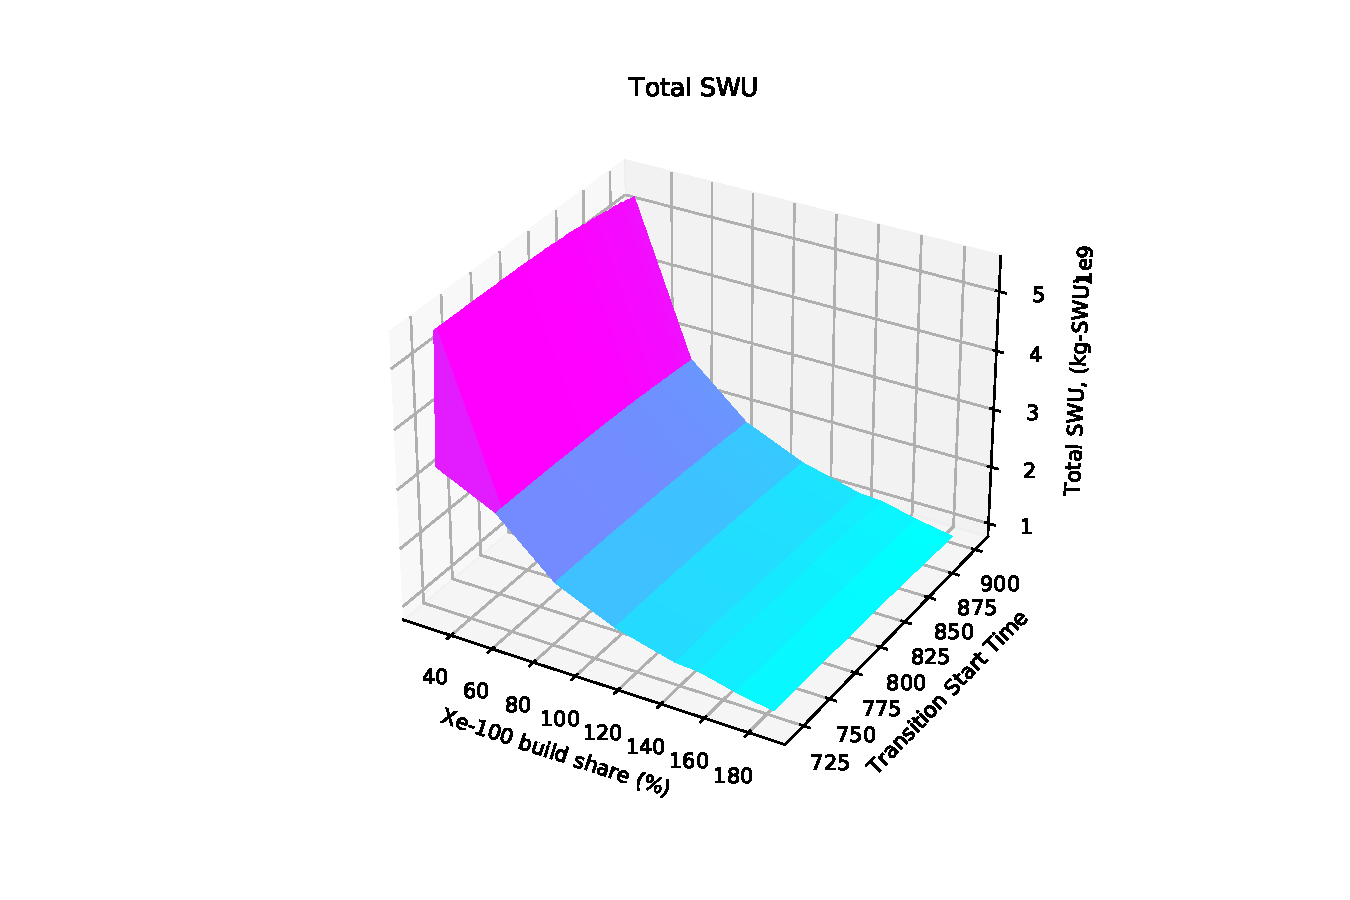
\includegraphics[width=\textwidth, trim=120 0 120 30, clip]{ts_xe100_burnup_swu.pdf}
        \caption{Effect on total SWU capacity.}
        \label{fig:ts_xe100_bu_swu}
    \end{subfigure}
    \hfill
    \begin{subfigure}[t]{0.48\textwidth}
        \centering
        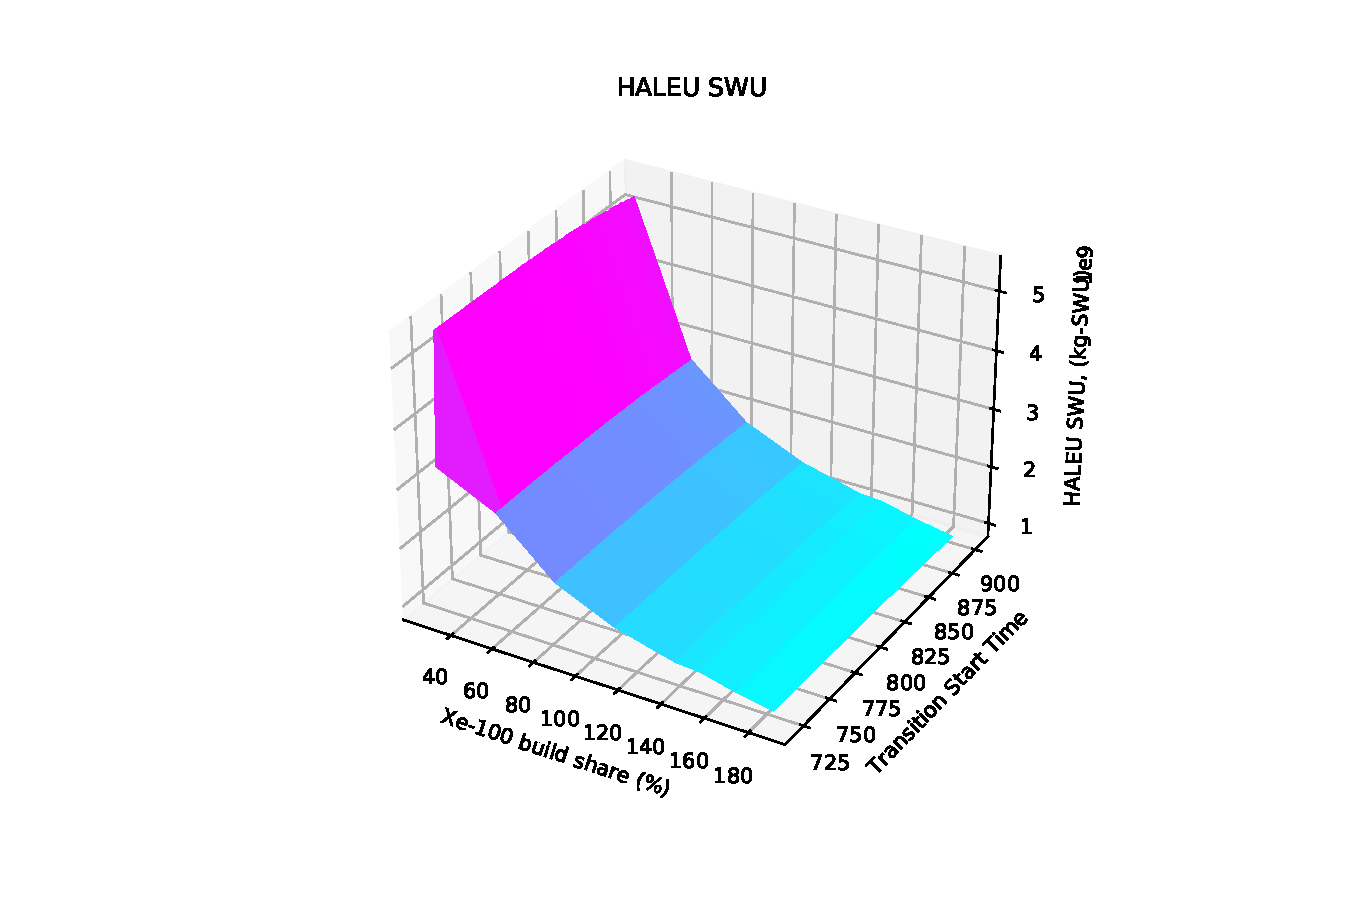
\includegraphics[width=\textwidth, trim=120 0 120 30, clip]{ts_xe100_burnup_haleu_swu.pdf}
        \caption{Effect on HALEU SWU capacity.}
        \label{fig:ts_xe100_bu_haleu_swu}
    \end{subfigure}
\end{figure}

\begin{figure}
    \ContinuedFloat    
    \begin{subfigure}[t]{0.48\textwidth}
        \centering
        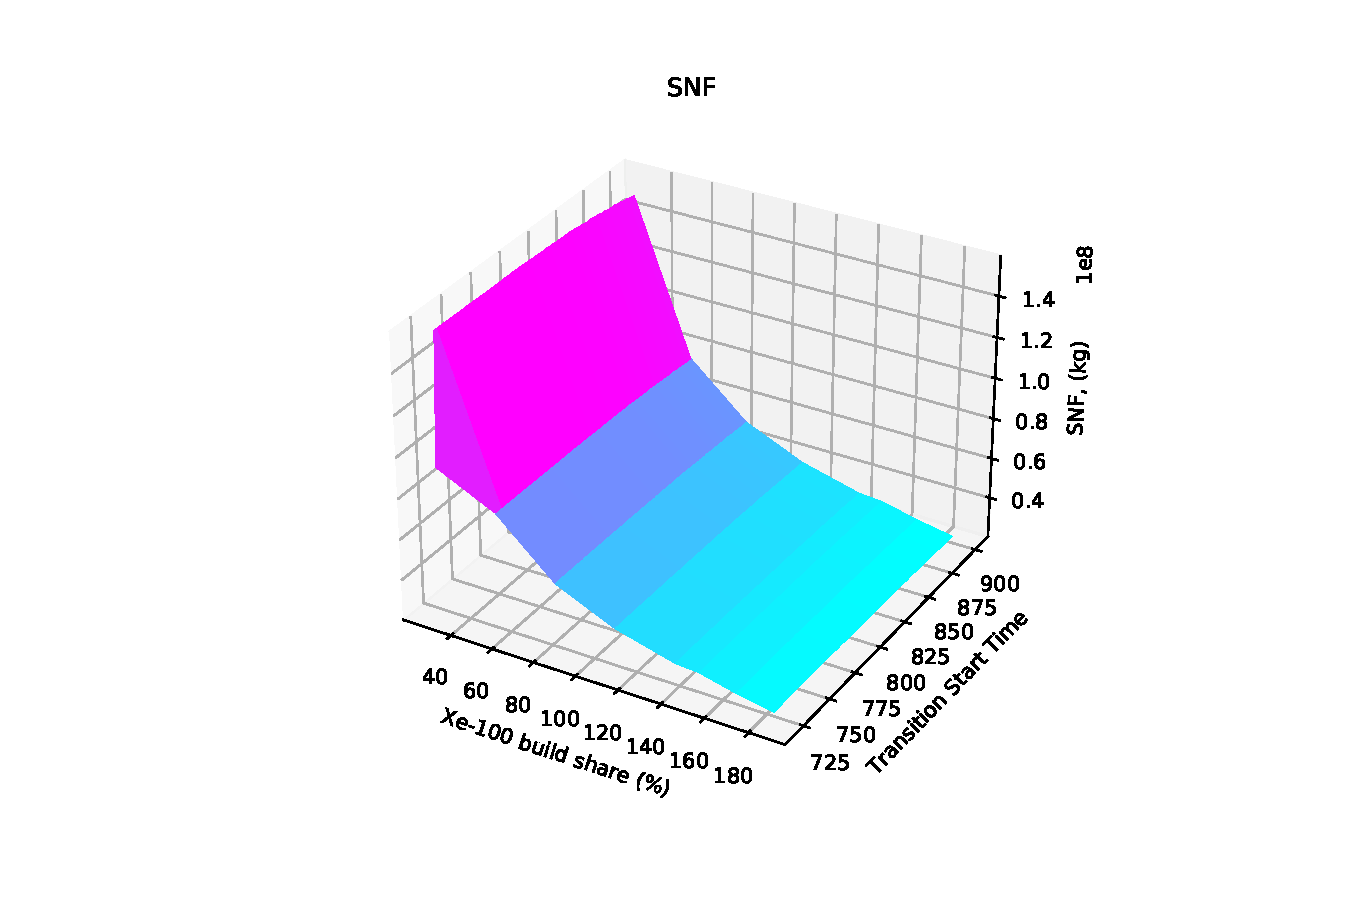
\includegraphics[width=\textwidth, trim=120 0 120 30, clip]{ts_xe100_burnup_waste.pdf}
        \caption{Effect on waste mass discharged.}
        \label{fig:ts_xe100_bu_waste}
    \end{subfigure}
    \hfill
    \begin{subfigure}[t]{0.48\textwidth}
        \centering
        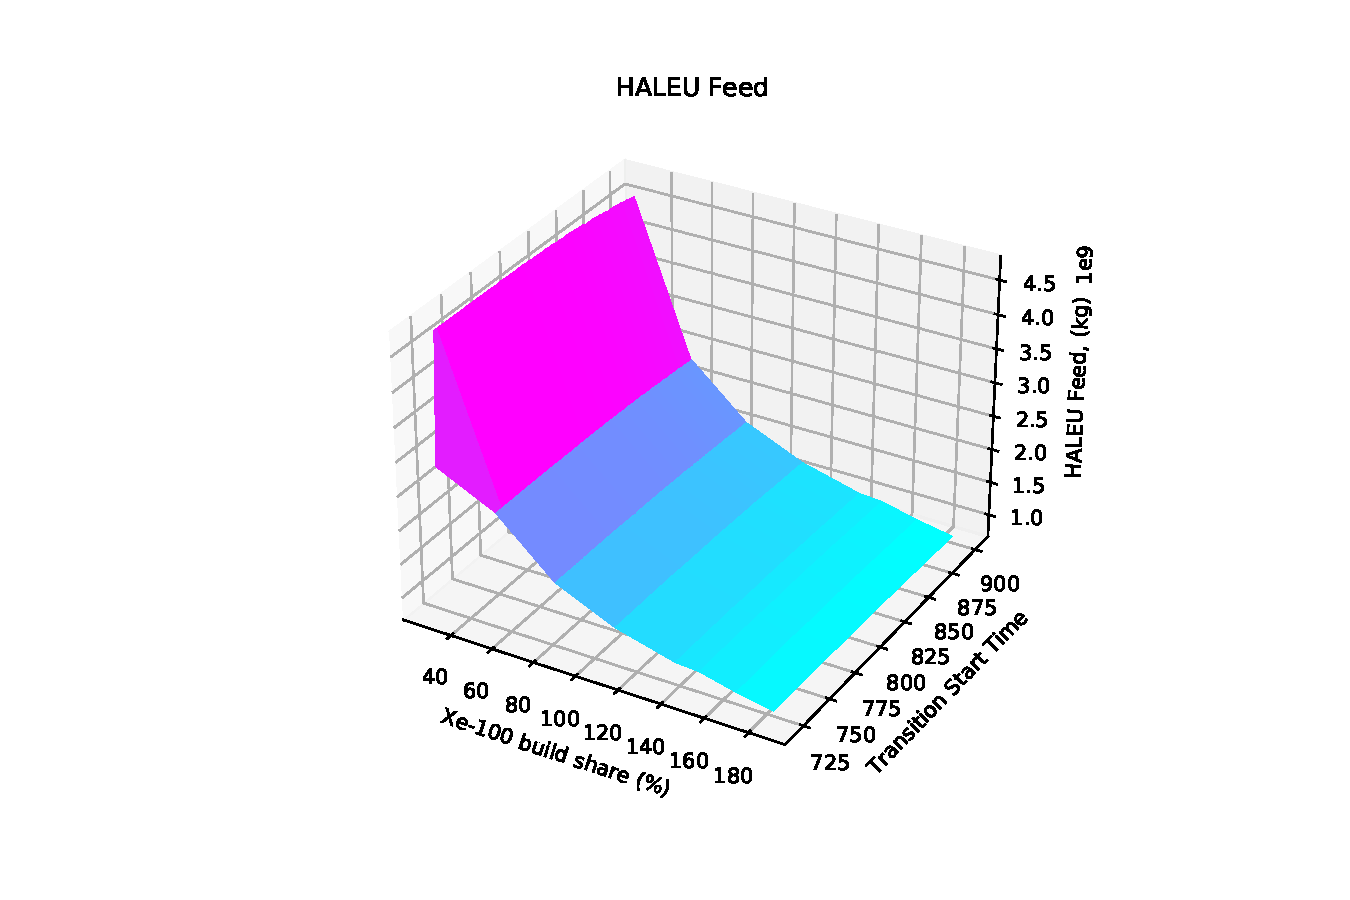
\includegraphics[width=\textwidth, trim=120 0 120 30, clip]{ts_xe100_burnup_feed.pdf}
        \caption{Effect on HALEU feed.}
        \label{fig:ts_xe100_bu_feed}
    \end{subfigure}
    \caption{Change in metrics resulting from variations in the 
    transition start time and Xe-100 burnup.}
    \label{fig:ts_xe100_bu}
\end{figure}

Figure \ref{fig:ts_mmr_bu} shows the effects of varying the transition 
start time and the \gls{MMR} discharge burnup on all six metrics. 

\begin{figure}
    \begin{subfigure}[t]{0.48\textwidth}
        \centering
        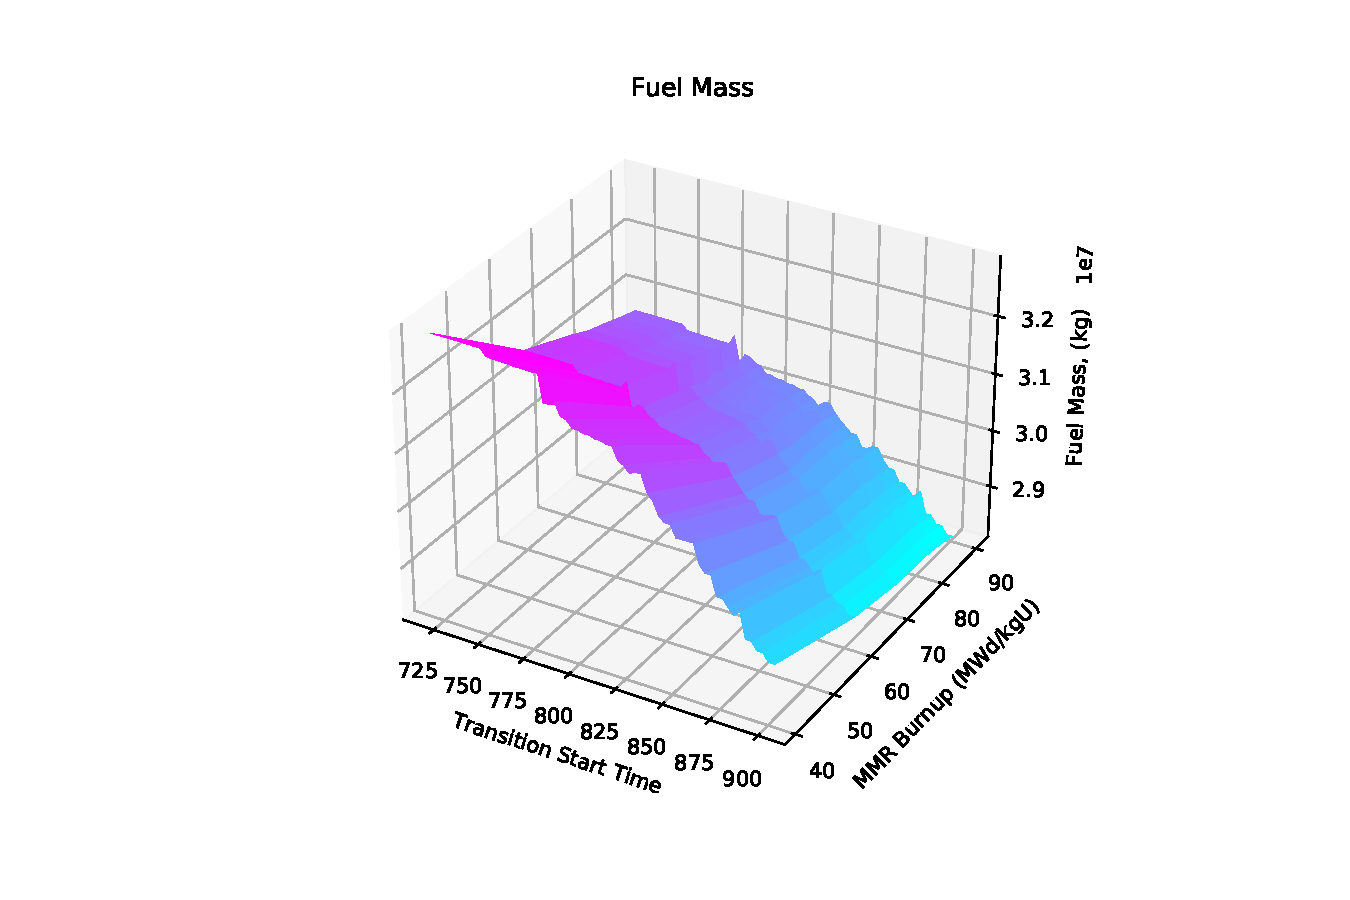
\includegraphics[width=\textwidth, trim=120 0 120 30, clip]{ts_mmr_burnup_enr_u.pdf}
        \caption{Effect on total fuel mass.}
        \label{fig:ts_mmr_bu_enr_u}
    \end{subfigure}
    \hfill
    \begin{subfigure}[t]{0.48\textwidth}
        \centering
        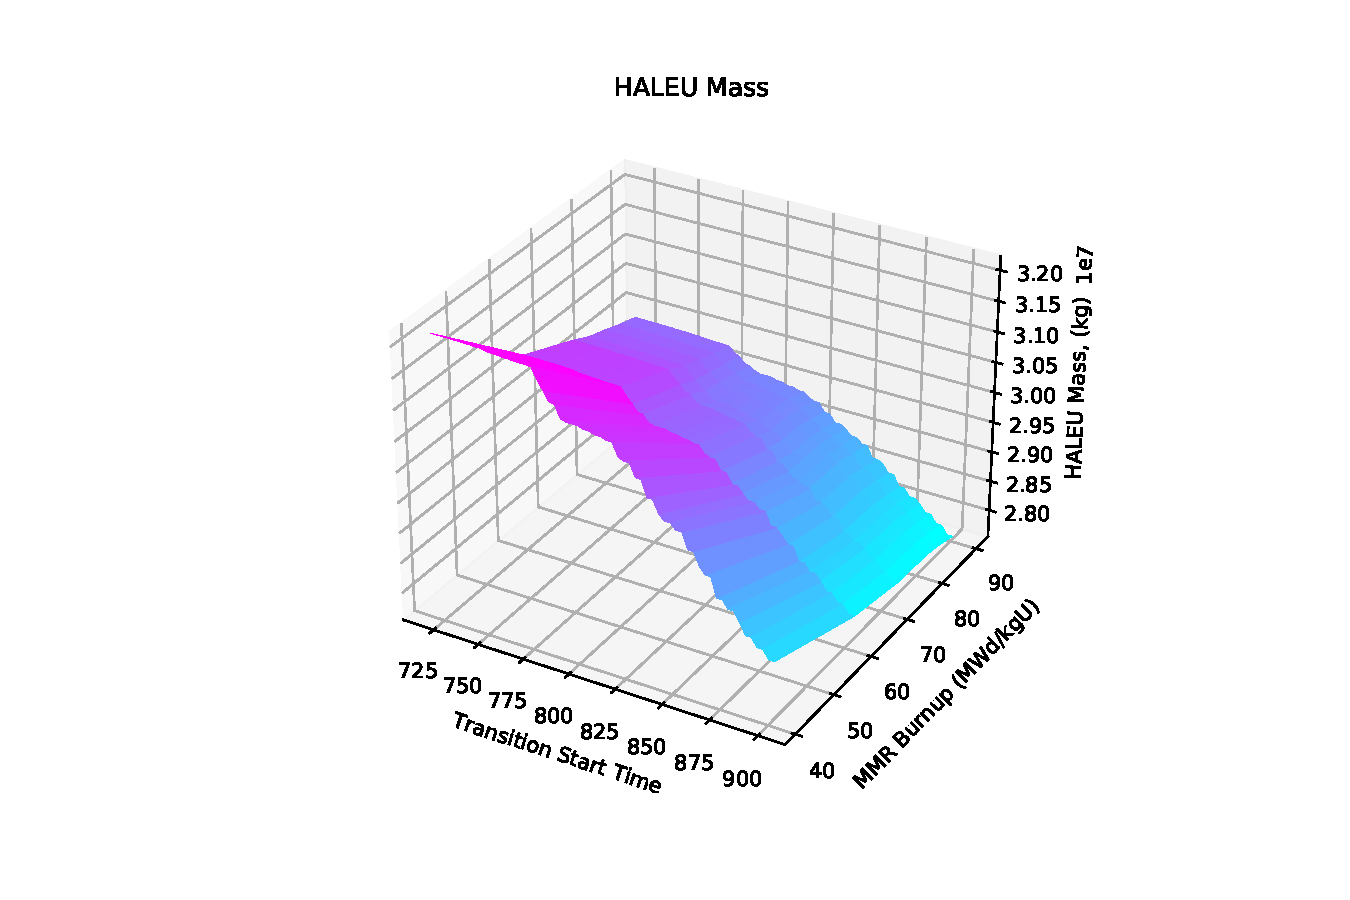
\includegraphics[width=\textwidth, trim=120 0 120 30, clip]{ts_mmr_burnup_haleu.pdf}
        \caption{Effect on HALEU mass.}
        \label{fig:ts_mmr_bu_haleu}
    \end{subfigure}
\end{figure}

\begin{figure}
    \ContinuedFloat    
    \begin{subfigure}[t]{0.48\textwidth}
        \centering
        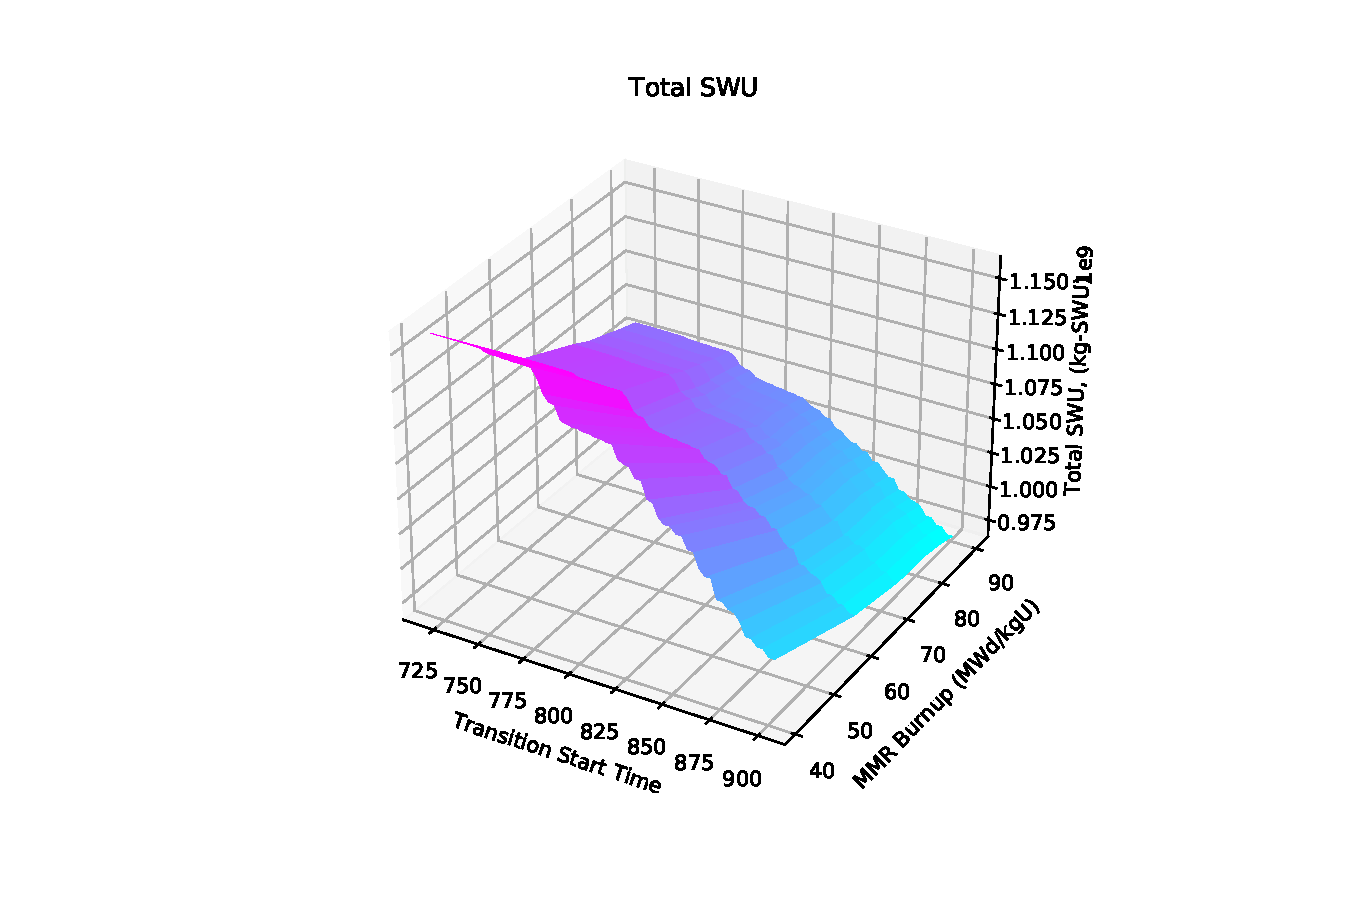
\includegraphics[width=\textwidth, trim=120 0 120 30, clip]{ts_mmr_burnup_swu.pdf}
        \caption{Effect on total SWU capacity.}
        \label{fig:ts_mmr_bu_swu}
    \end{subfigure}
    \hfill
    \begin{subfigure}[t]{0.48\textwidth}
        \centering
        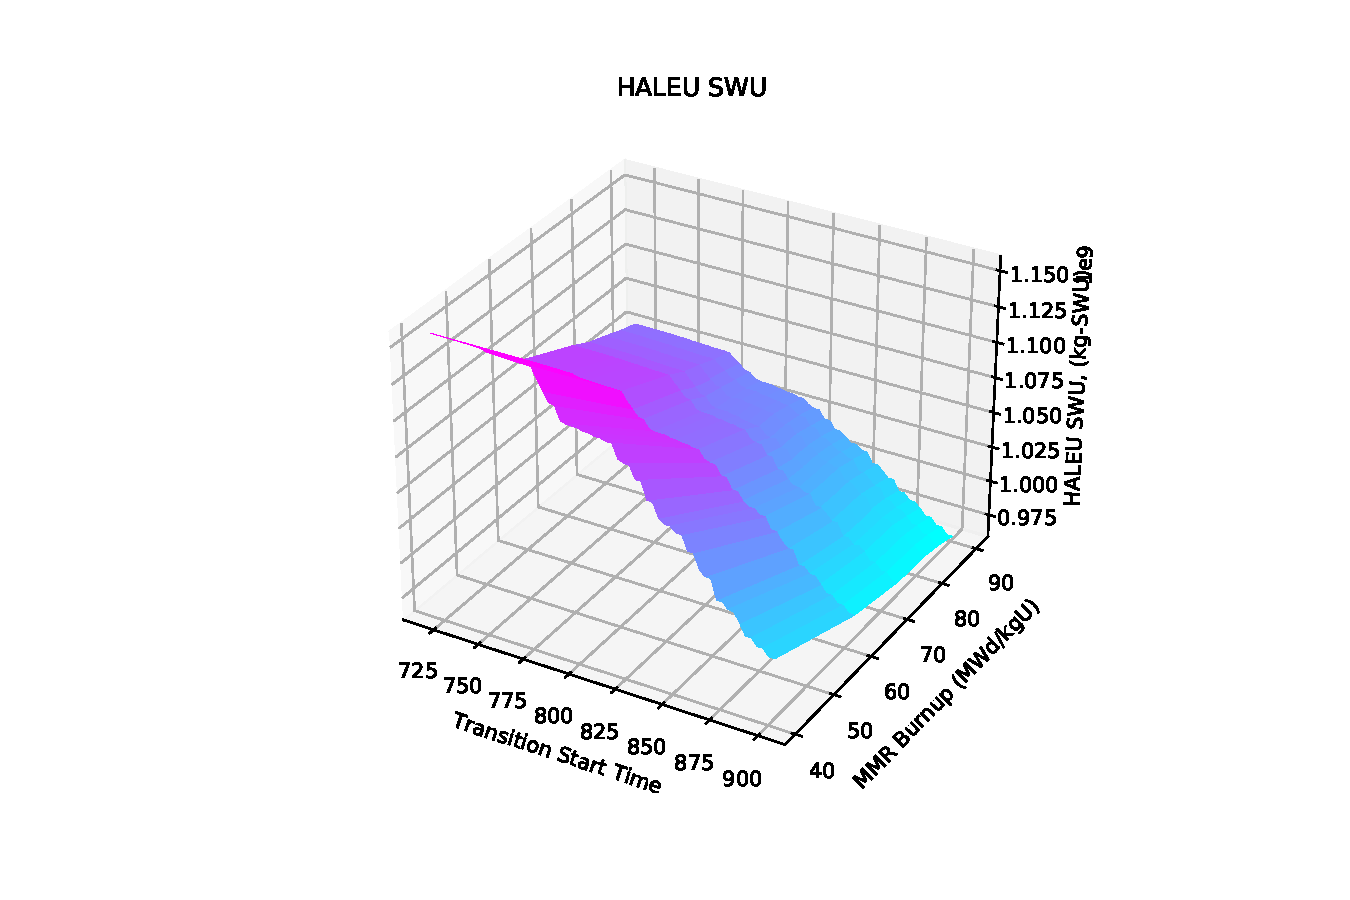
\includegraphics[width=\textwidth, trim=120 0 120 30, clip]{ts_mmr_burnup_haleu_swu.pdf}
        \caption{Effect on HALEU SWU capacity.}
        \label{fig:ts_mmr_bu_haleu_swu}
    \end{subfigure}
    
    \begin{subfigure}[t]{0.48\textwidth}
        \centering
        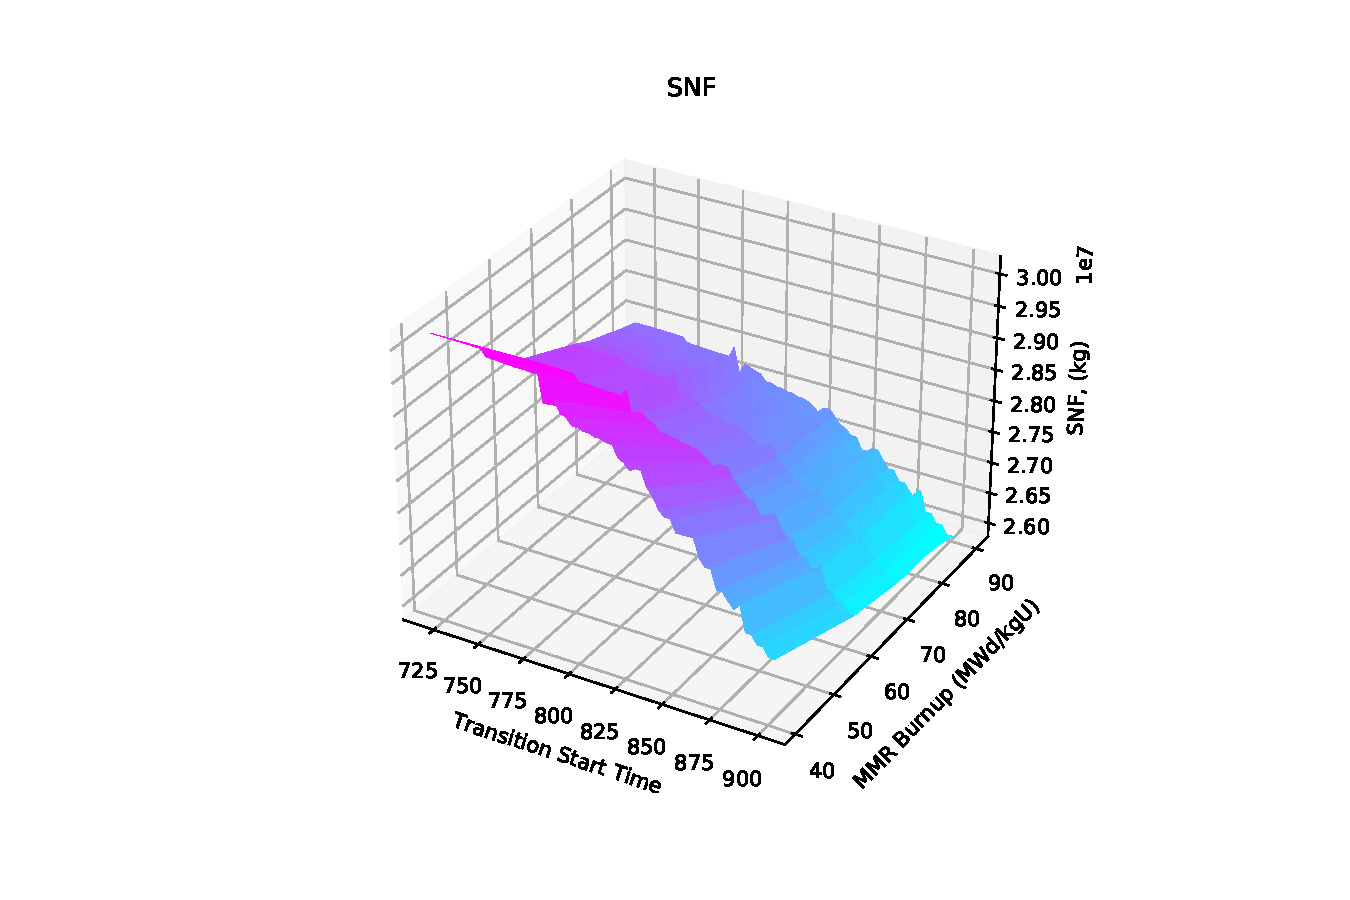
\includegraphics[width=\textwidth, trim=120 0 120 30, clip]{ts_mmr_burnup_waste.pdf}
        \caption{Effect on waste mass discharged.}
        \label{fig:ts_mmr_bu_waste}
    \end{subfigure}
    \hfill
    \begin{subfigure}[t]{0.48\textwidth}
        \centering
        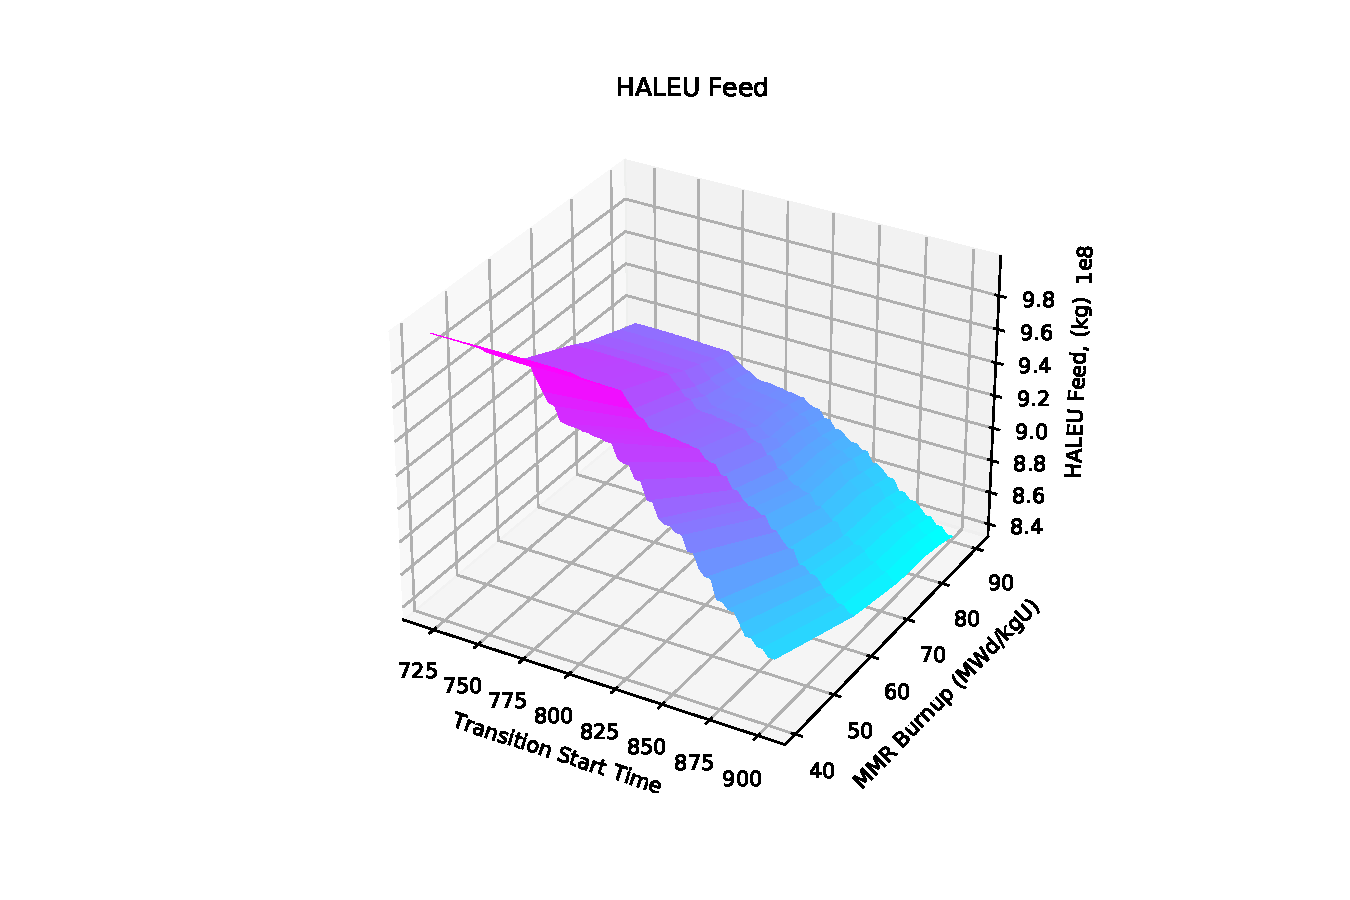
\includegraphics[width=\textwidth, trim=120 0 120 30, clip]{ts_mmr_burnup_feed.pdf}
        \caption{Effect on HALEU feed.}
        \label{fig:ts_mmr_bu_feed}
    \end{subfigure}
    \caption{Change in metrics resulting from variations in the 
    transition start time and MMR burnup.}
    \label{fig:ts_mmr_bu}
\end{figure}

Figure \ref{fig:lwr_xe100_share} shows the effects of varying the 
percent of \glspl{LWR} operating for 80 years and the Xe-100 
build share on all six metrics. The trends observed in the \gls{OAT} 
can also be observed here, such as how increasing the Xe-100 share 
increases the \gls{HALEU} mass required but increasing the 
percent of \glspl{LWR} decreases this metric. However, these results 
show that there is a combined effect from varying these parameters 
together that is not captured in the \gls{OAT} analysis. For 
example, the \gls{HALEU} mass decreases by a greater fraction 
as the percent of \glspl{LWR} and Xe-100 build shares increase than 
when only the percent of \glspl{LWR} extended increases. This combined 
effect is a result of more of the advanced reactor fleet being fueled 
by \gls{HALEU}-fueled reactors. However, these results also show that 
the despite this combined effect, not deploying Xe-100s will still
result in a minimum in the \gls{HALEU} mass required. 

\begin{figure}
    \begin{subfigure}[t]{0.48\textwidth}
        \centering
        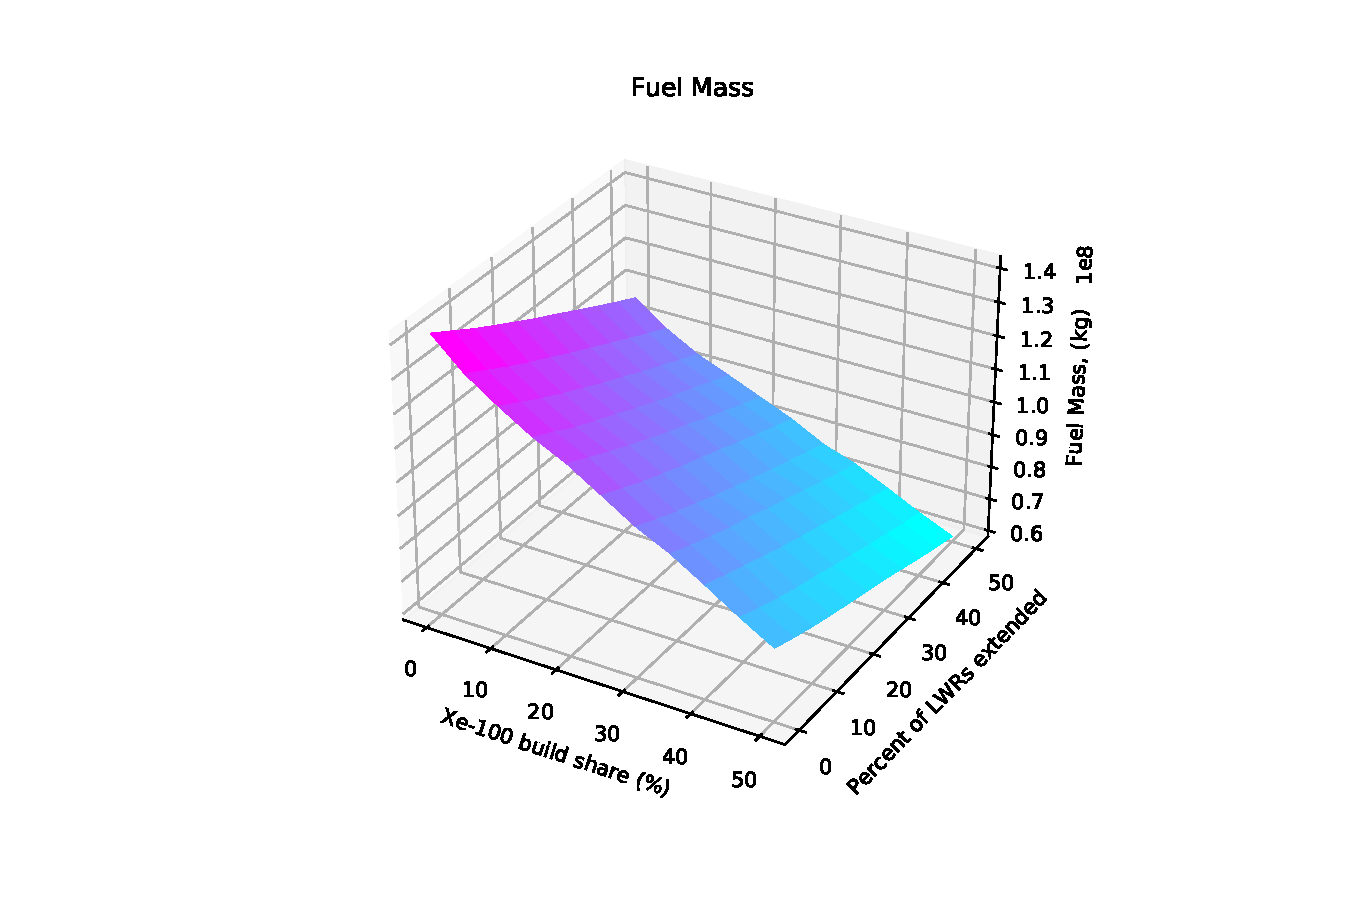
\includegraphics[width=\textwidth, trim=120 0 120 30, clip]{lwr_xe100_share_enr_u.pdf}
        \caption{Effect on total fuel mass.}
        \label{fig:lwr_xe100_share_enr_u}
    \end{subfigure}
    \hfill
    \begin{subfigure}[t]{0.48\textwidth}
        \centering
        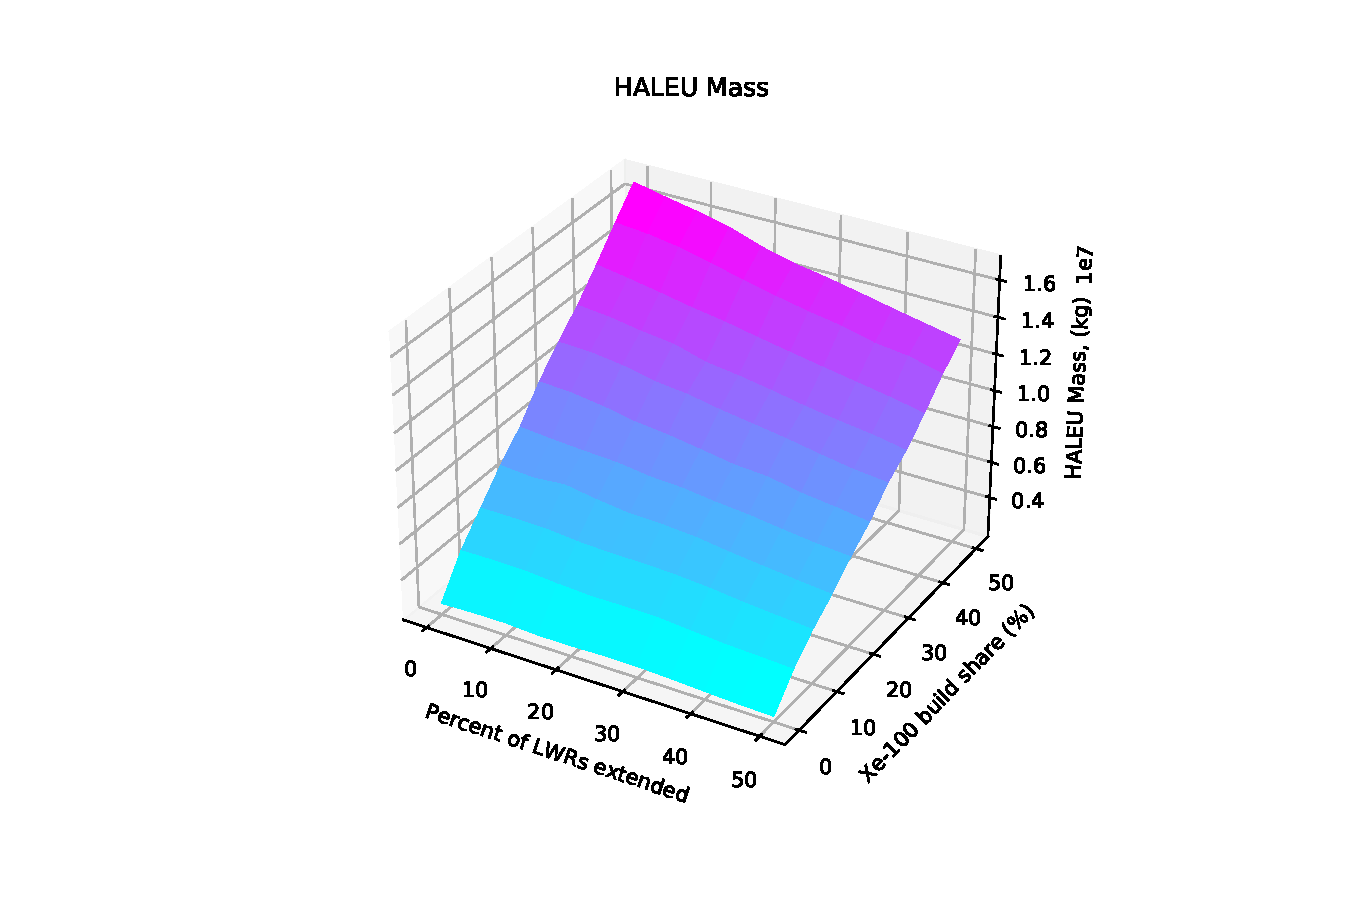
\includegraphics[width=\textwidth, trim=120 0 120 30, clip]{lwr_xe100_share_haleu.pdf}
        \caption{Effect on HALEU mass.}
        \label{fig:lwr_xe100_share_haleu}
    \end{subfigure}  
    \begin{subfigure}[t]{0.48\textwidth}
        \centering
        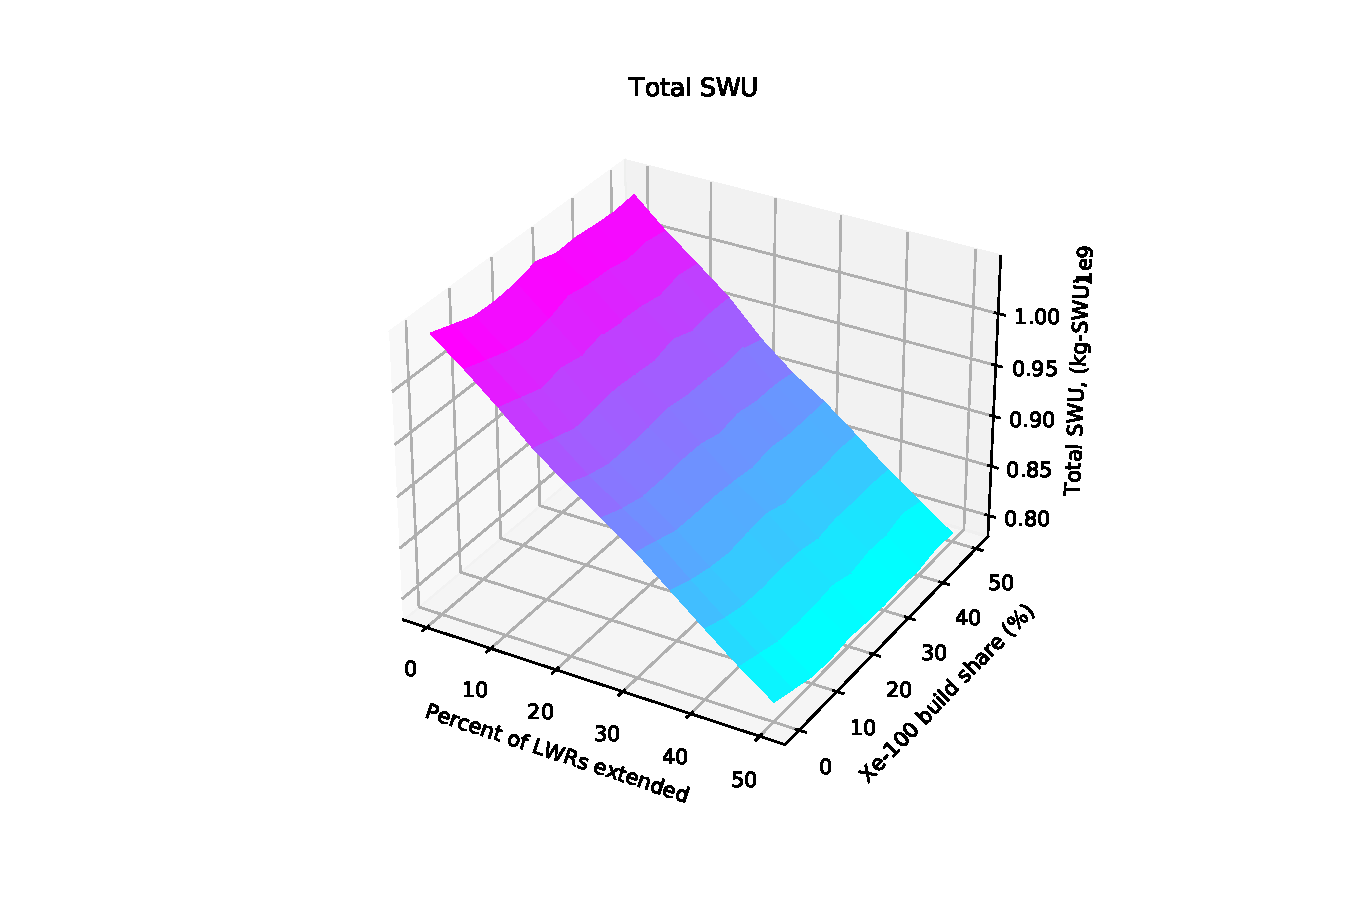
\includegraphics[width=\textwidth, trim=120 0 120 30, clip]{lwr_xe100_share_swu.pdf}
        \caption{Effect on total SWU capacity.}
        \label{fig:lwr_xe100_share_swu}
    \end{subfigure}
    \hfill
    \begin{subfigure}[t]{0.48\textwidth}
        \centering
        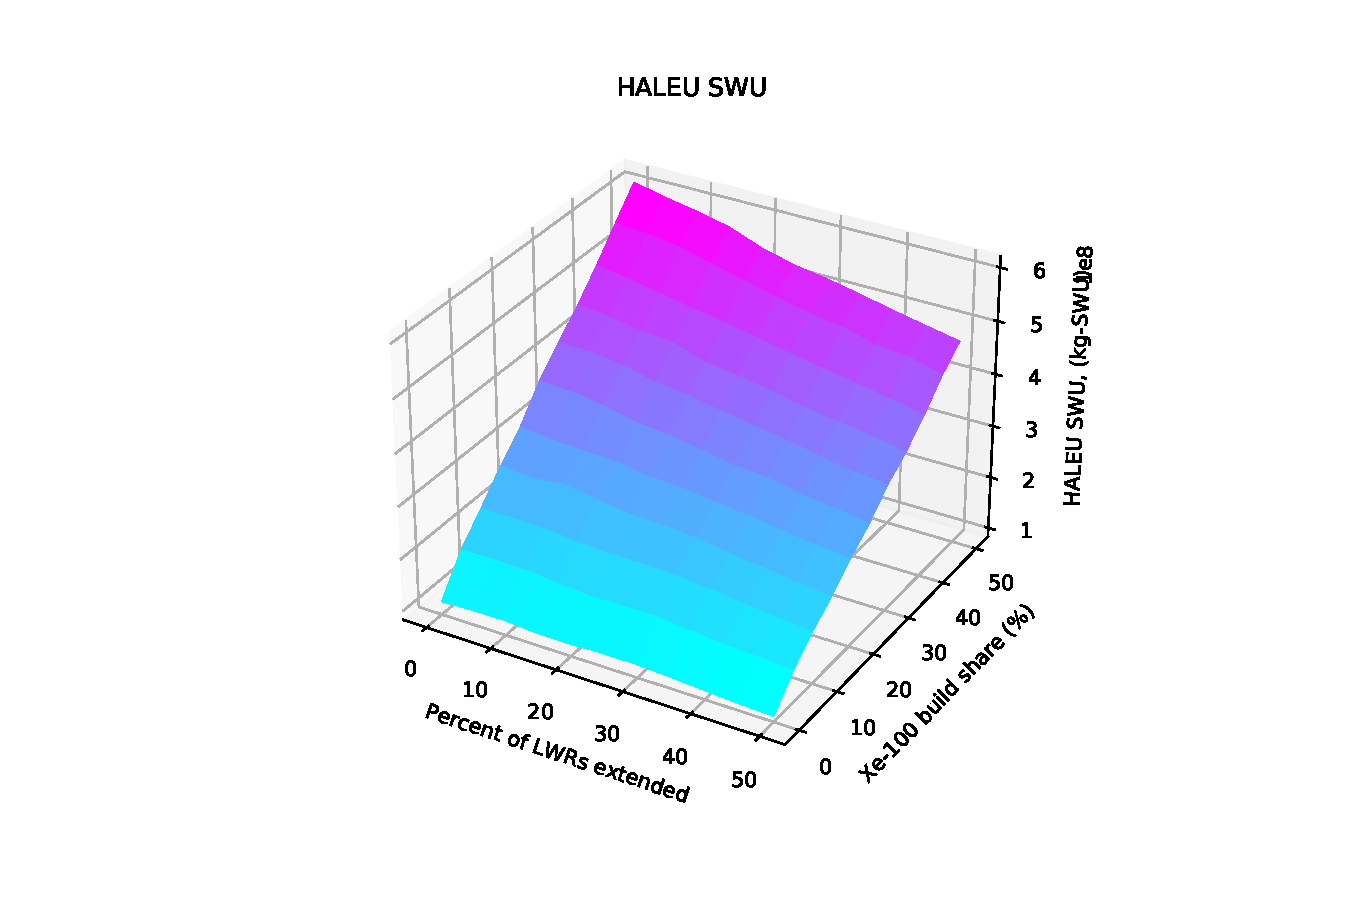
\includegraphics[width=\textwidth, trim=120 0 120 30, clip]{lwr_xe100_share_haleu_swu.pdf}
        \caption{Effect on HALEU SWU capacity.}
        \label{fig:lwr_xe100_share_haleu_swu}
    \end{subfigure}
\end{figure}

\begin{figure}
    \ContinuedFloat    
    \begin{subfigure}[t]{0.48\textwidth}
        \centering
        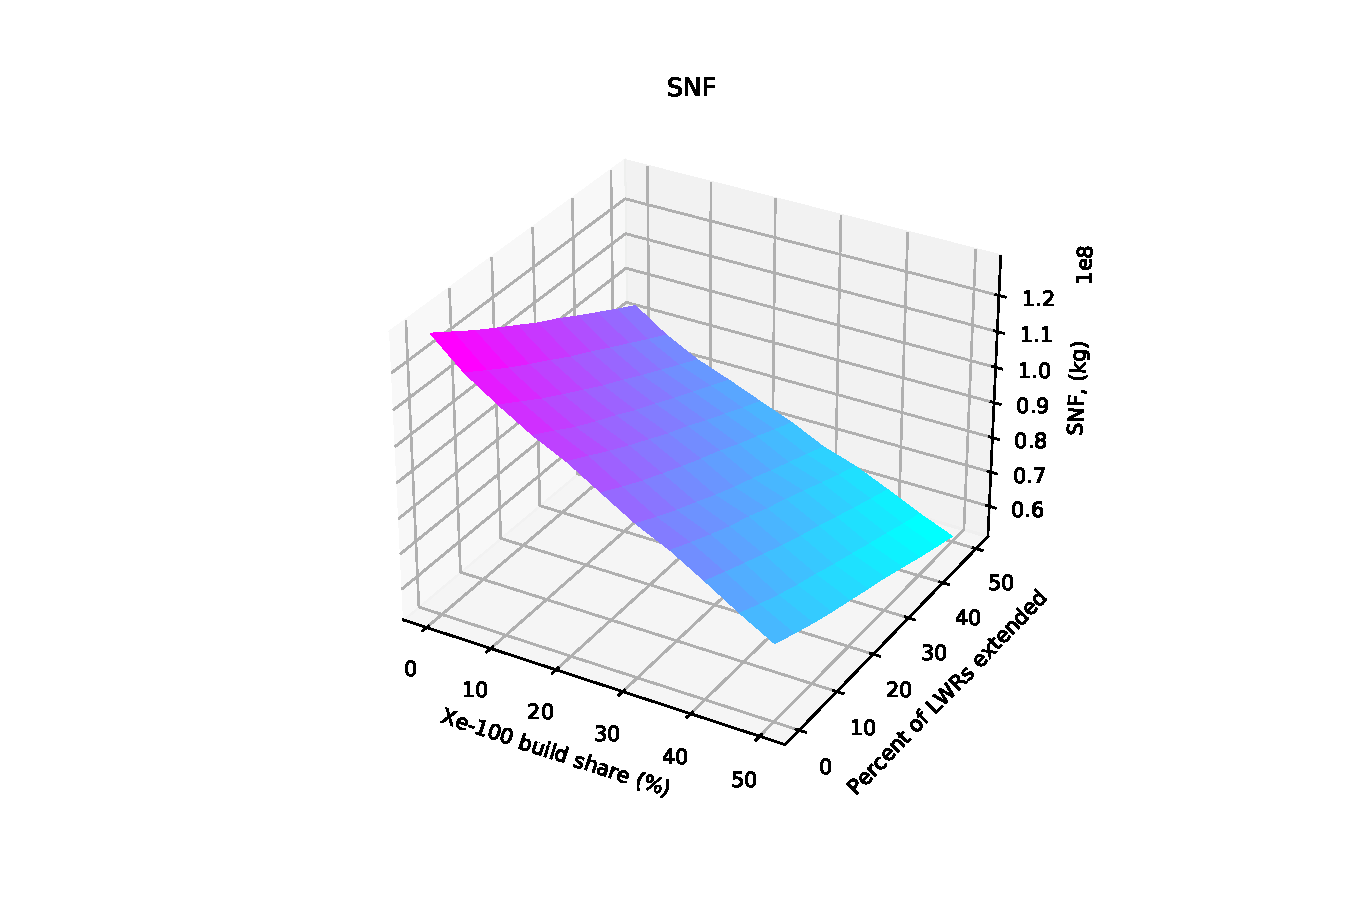
\includegraphics[width=\textwidth, trim=120 0 120 30, clip]{lwr_xe100_share_waste.pdf}
        \caption{Effect on waste mass discharged.}
        \label{fig:lwr_xe100_share_waste}
    \end{subfigure}
    \hfill
    \begin{subfigure}[t]{0.48\textwidth}
        \centering
        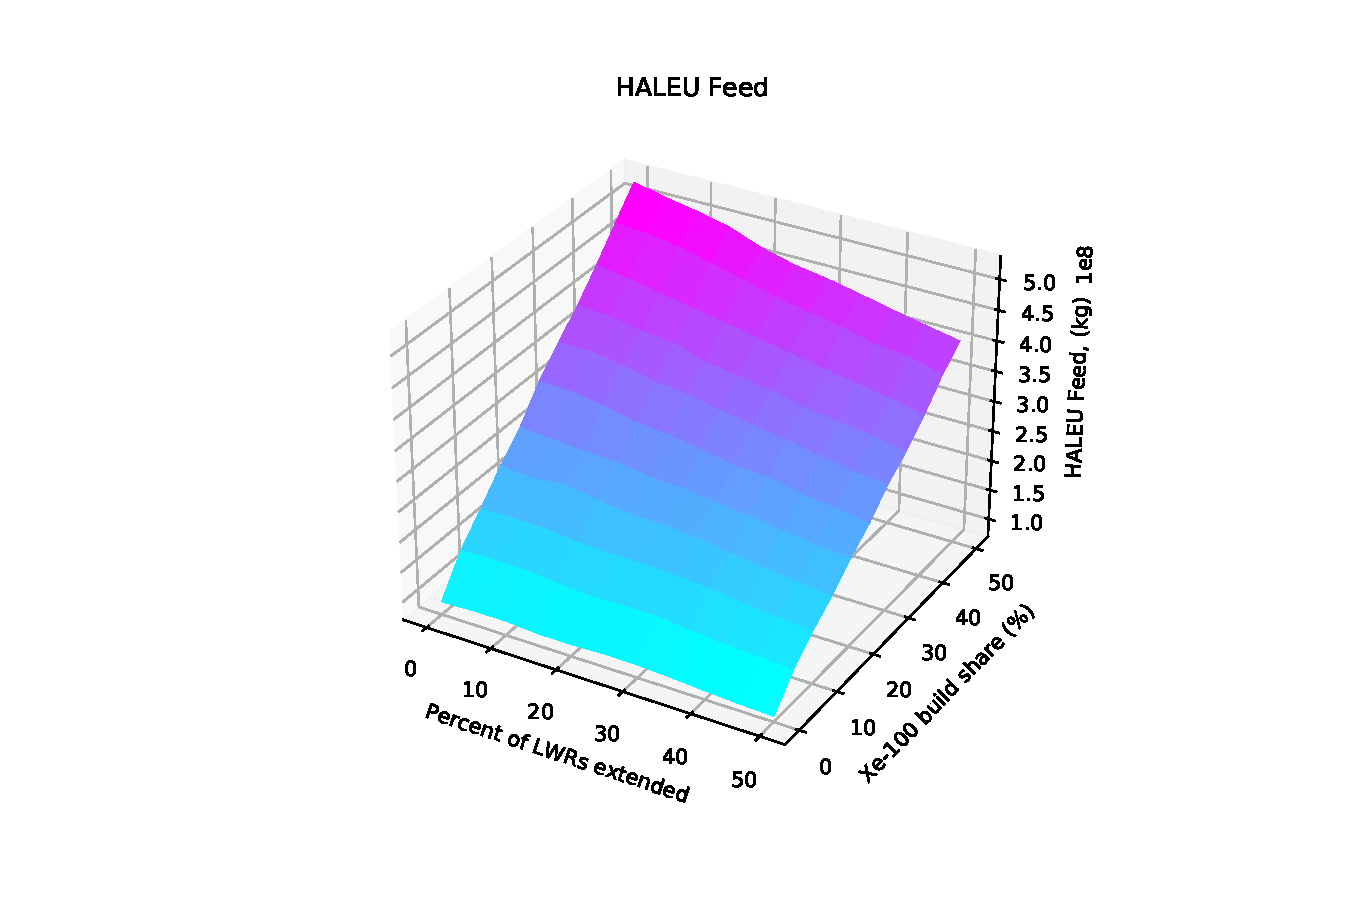
\includegraphics[width=\textwidth, trim=120 0 120 30, clip]{lwr_xe100_share_feed.pdf}
        \caption{Effect on HALEU feed.}
        \label{fig:lwr_xe100_share_feed}
    \end{subfigure}
    \caption{Change in metrics resulting from variations in the 
    LWR lifetimes and Xe-100 build share.}
    \label{fig:lwr_xe100_share}
\end{figure}

\begin{figure}
    \begin{subfigure}[t]{0.48\textwidth}
        \centering
        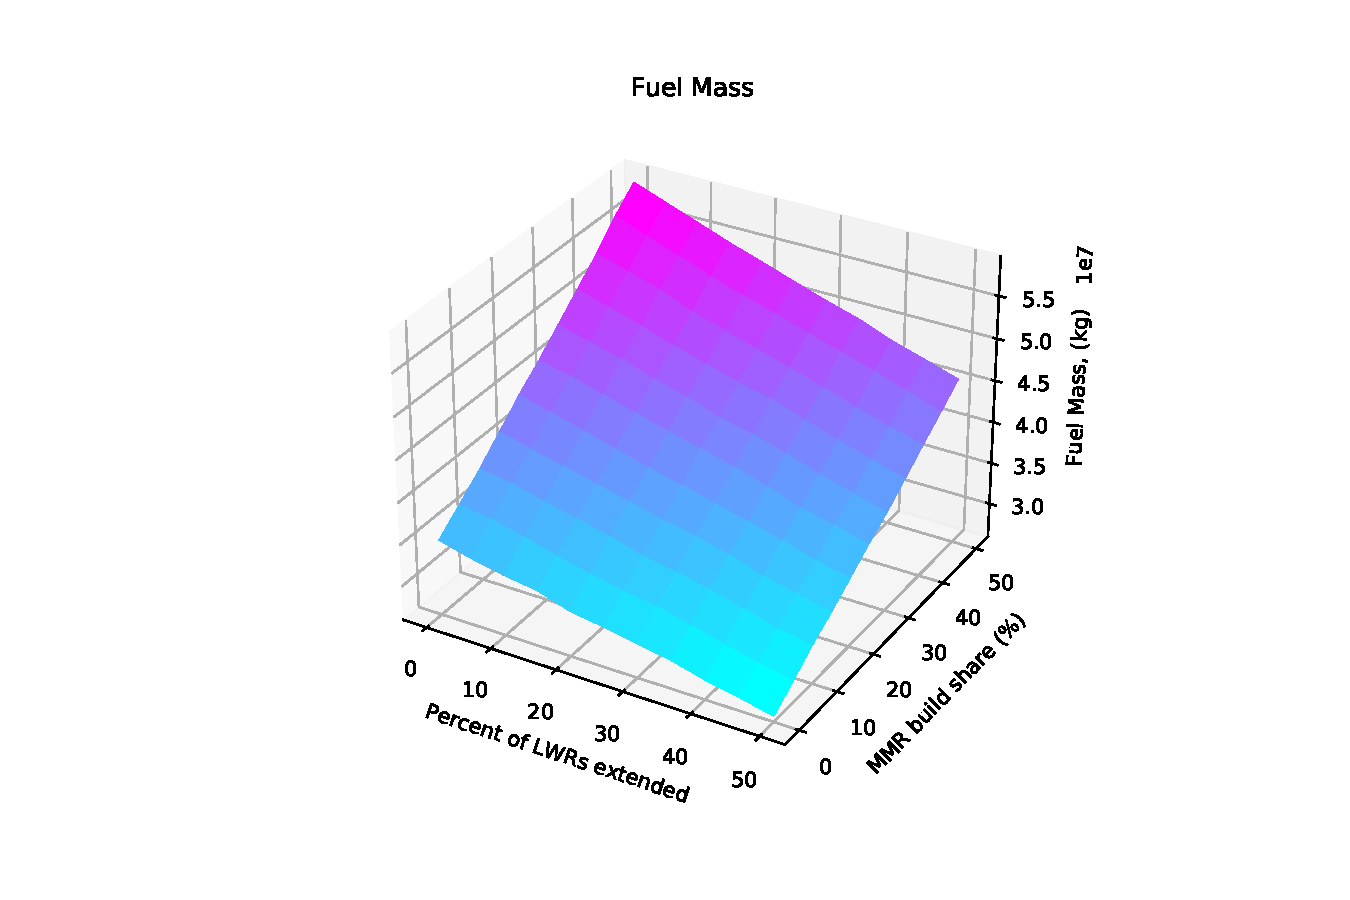
\includegraphics[width=\textwidth, trim=120 0 120 30, clip]{lwr_mmr_share_enr_u.pdf}
        \caption{Effect on total fuel mass.}
        \label{fig:lwr_mmr_share_enr_u}
    \end{subfigure}
    \hfill
    \begin{subfigure}[t]{0.48\textwidth}
        \centering
        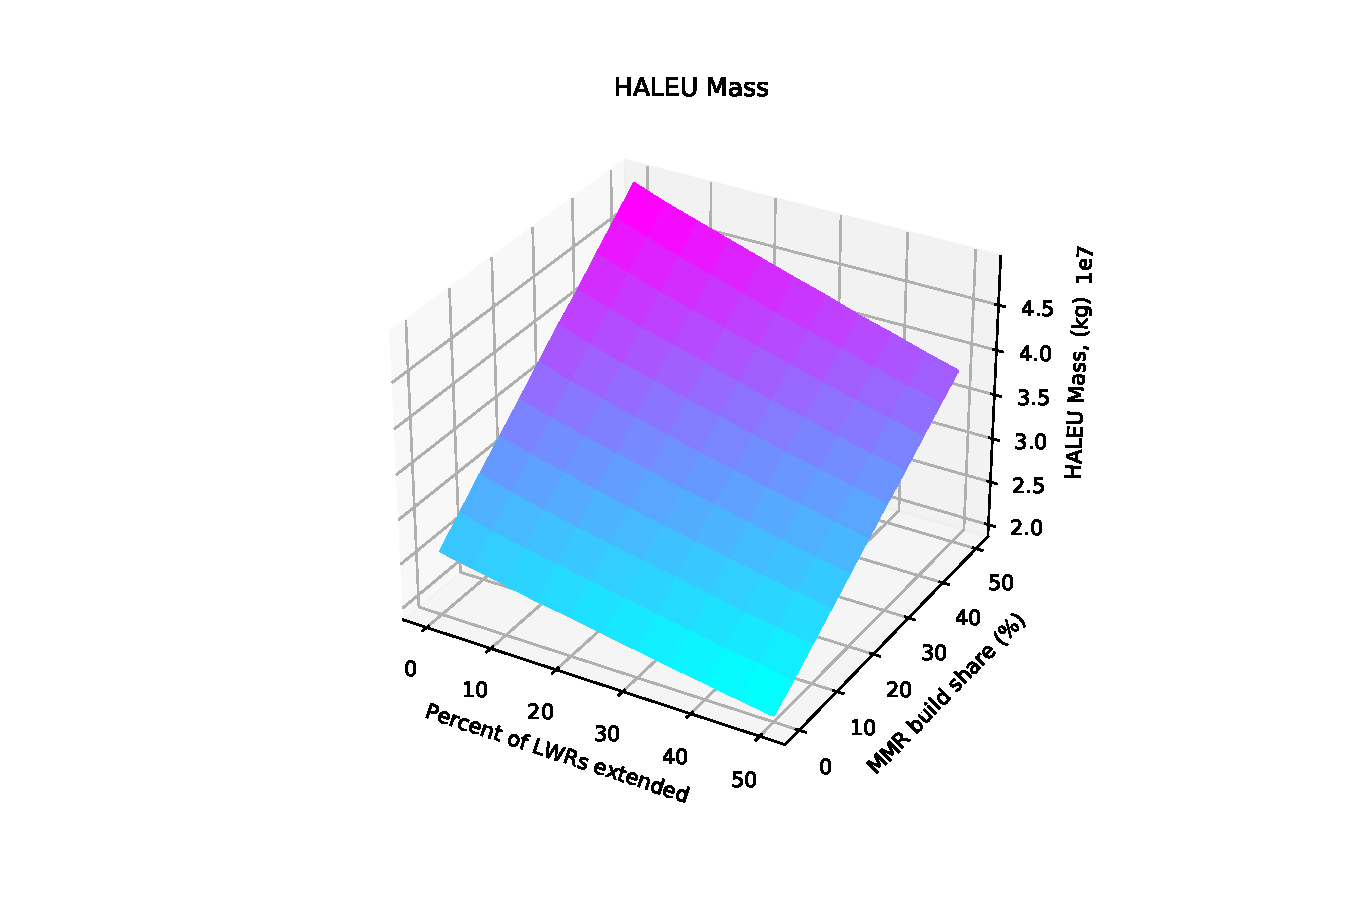
\includegraphics[width=\textwidth, trim=120 0 120 30, clip]{lwr_mmr_share_haleu.pdf}
        \caption{Effect on HALEU mass.}
        \label{fig:lwr_mmr_share_haleu}
    \end{subfigure}
\end{figure}

\begin{figure}
    \ContinuedFloat    
    \begin{subfigure}[t]{0.48\textwidth}
        \centering
        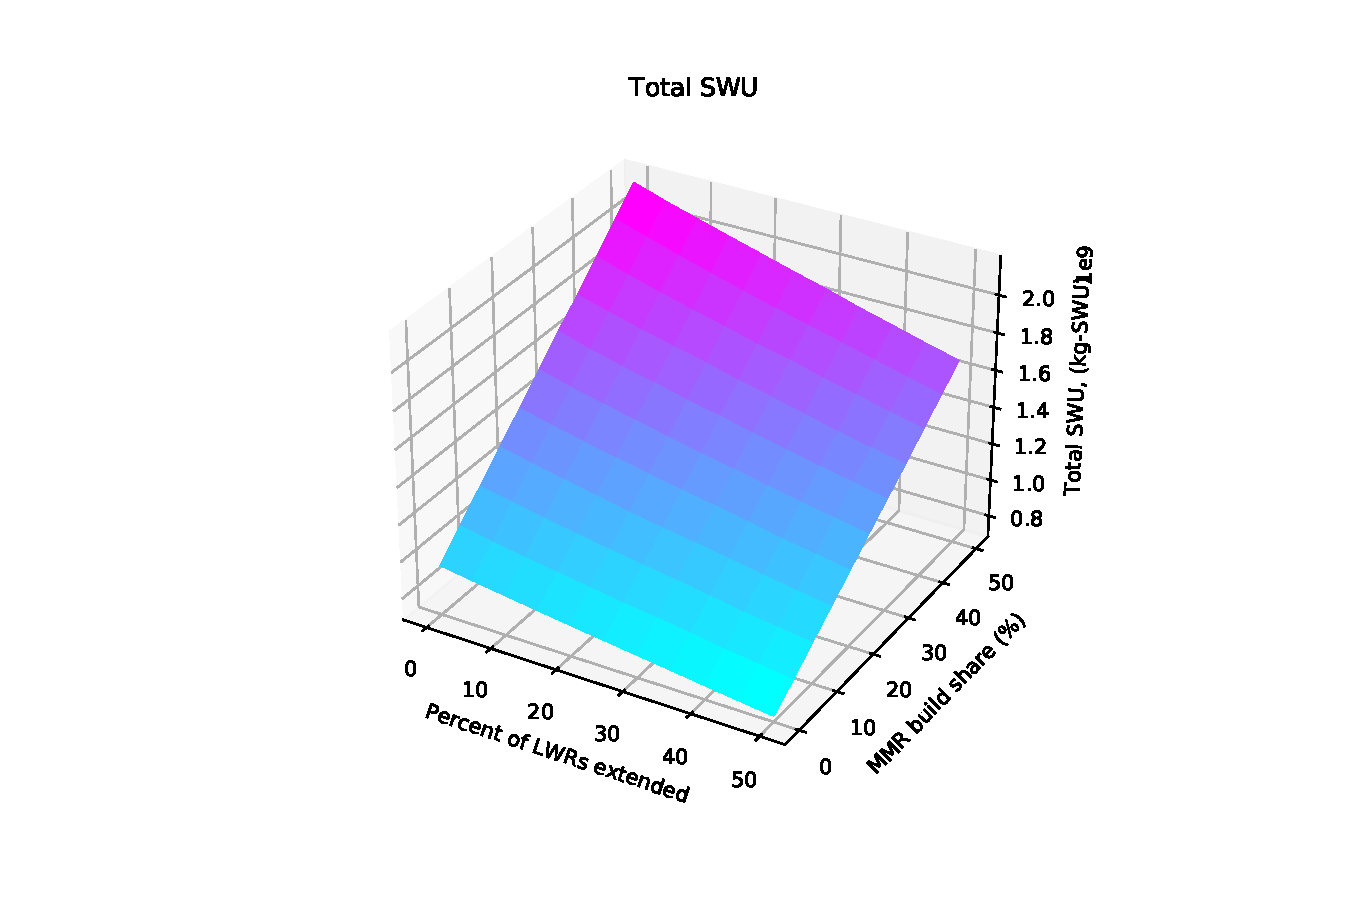
\includegraphics[width=\textwidth, trim=120 0 120 30, clip]{lwr_mmr_share_swu.pdf}
        \caption{Effect on total SWU capacity.}
        \label{fig:lwr_mmr_share_swu}
    \end{subfigure}
    \hfill
    \begin{subfigure}[t]{0.48\textwidth}
        \centering
        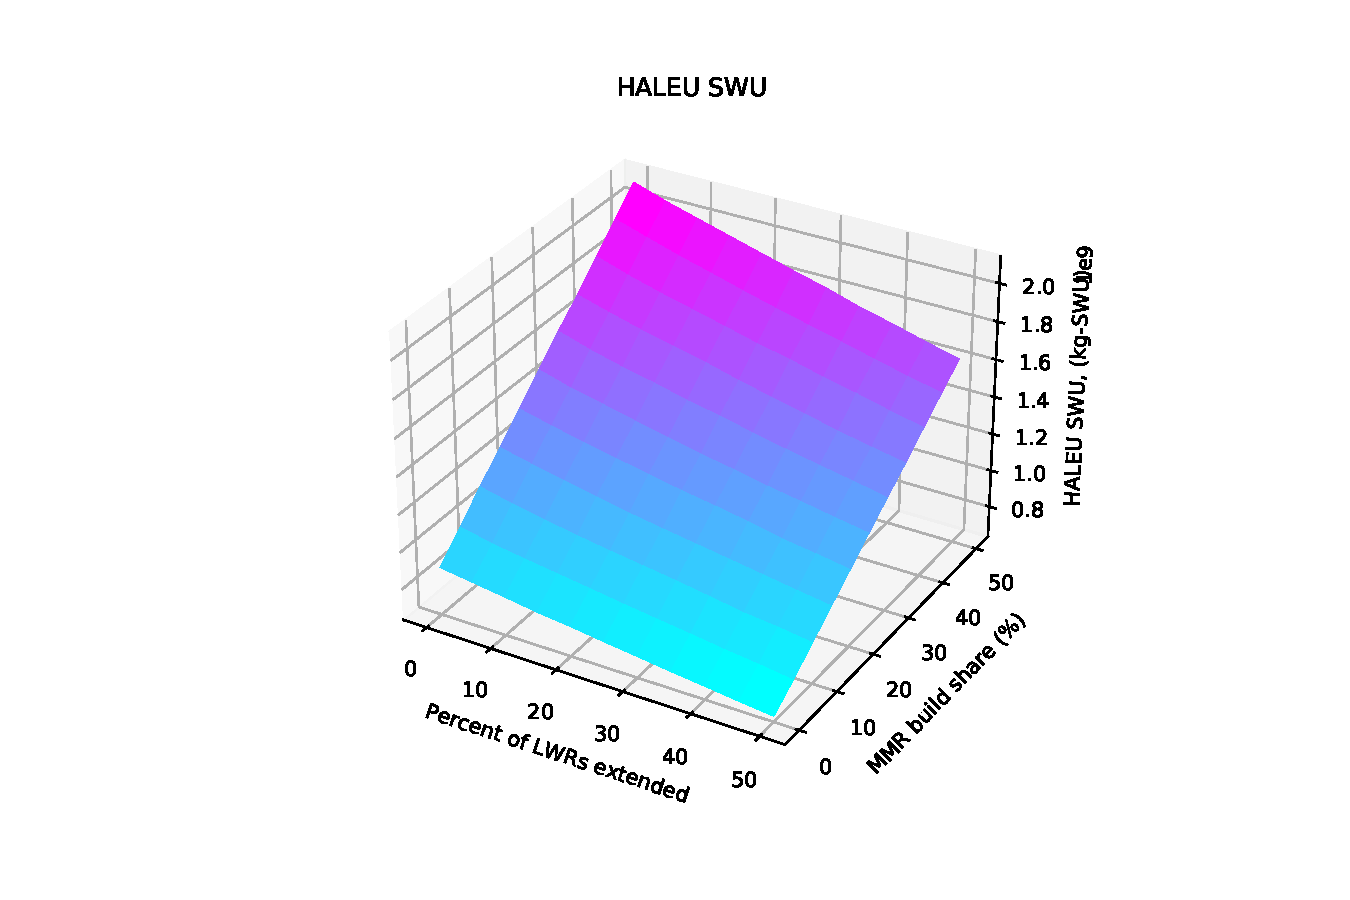
\includegraphics[width=\textwidth, trim=120 0 120 30, clip]{lwr_mmr_share_haleu_swu.pdf}
        \caption{Effect on HALEU SWU capacity.}
        \label{fig:lwr_mmr_share_haleu_swu}
    \end{subfigure}

    \begin{subfigure}[t]{0.48\textwidth}
        \centering
        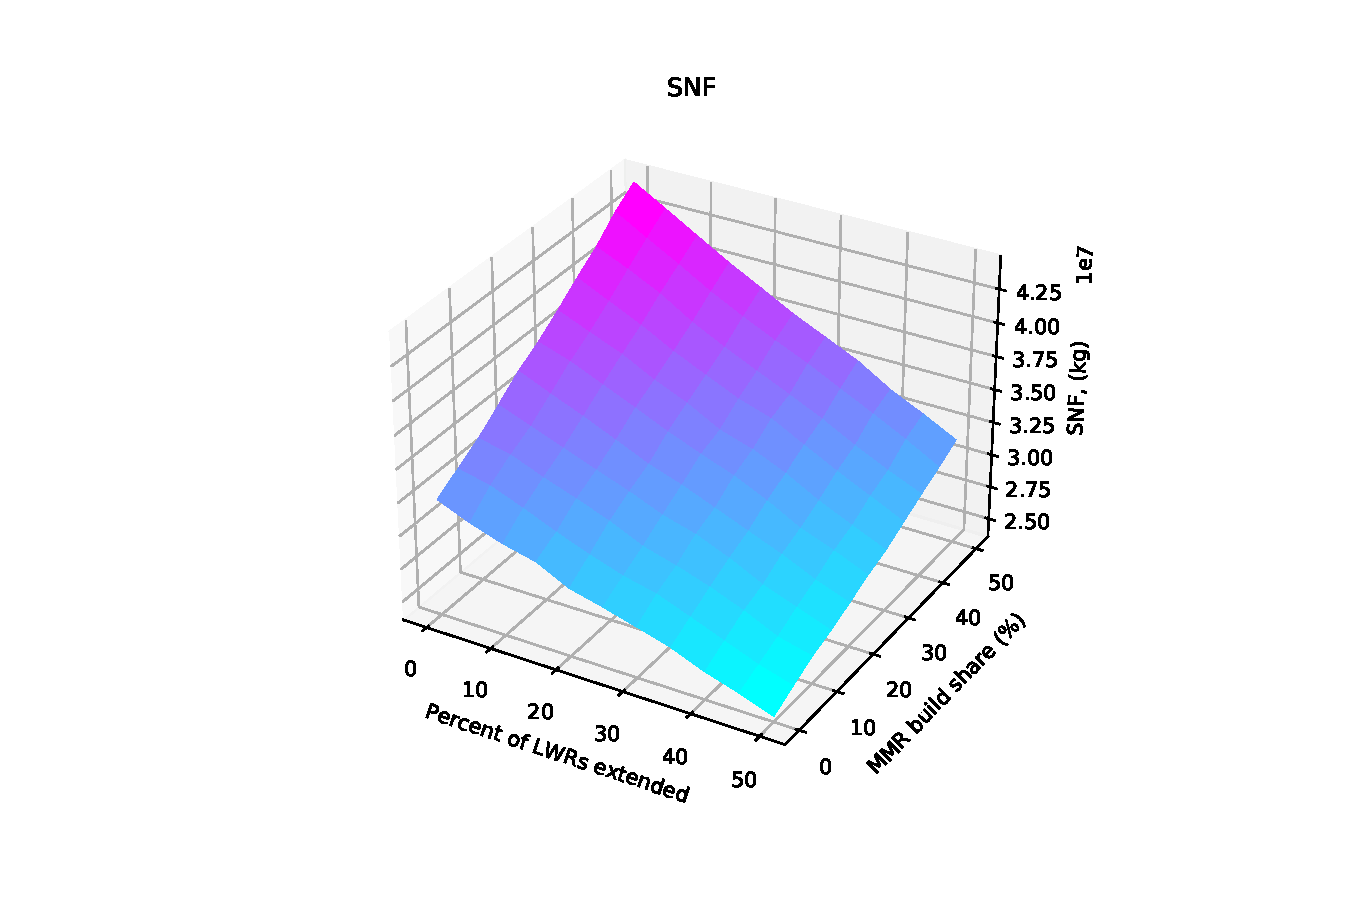
\includegraphics[width=\textwidth, trim=120 0 120 30, clip]{lwr_mmr_share_waste.pdf}
        \caption{Effect on waste mass discharged.}
        \label{fig:lwr_mmr_share_waste}
    \end{subfigure}
    \hfill
    \begin{subfigure}[t]{0.48\textwidth}
        \centering
        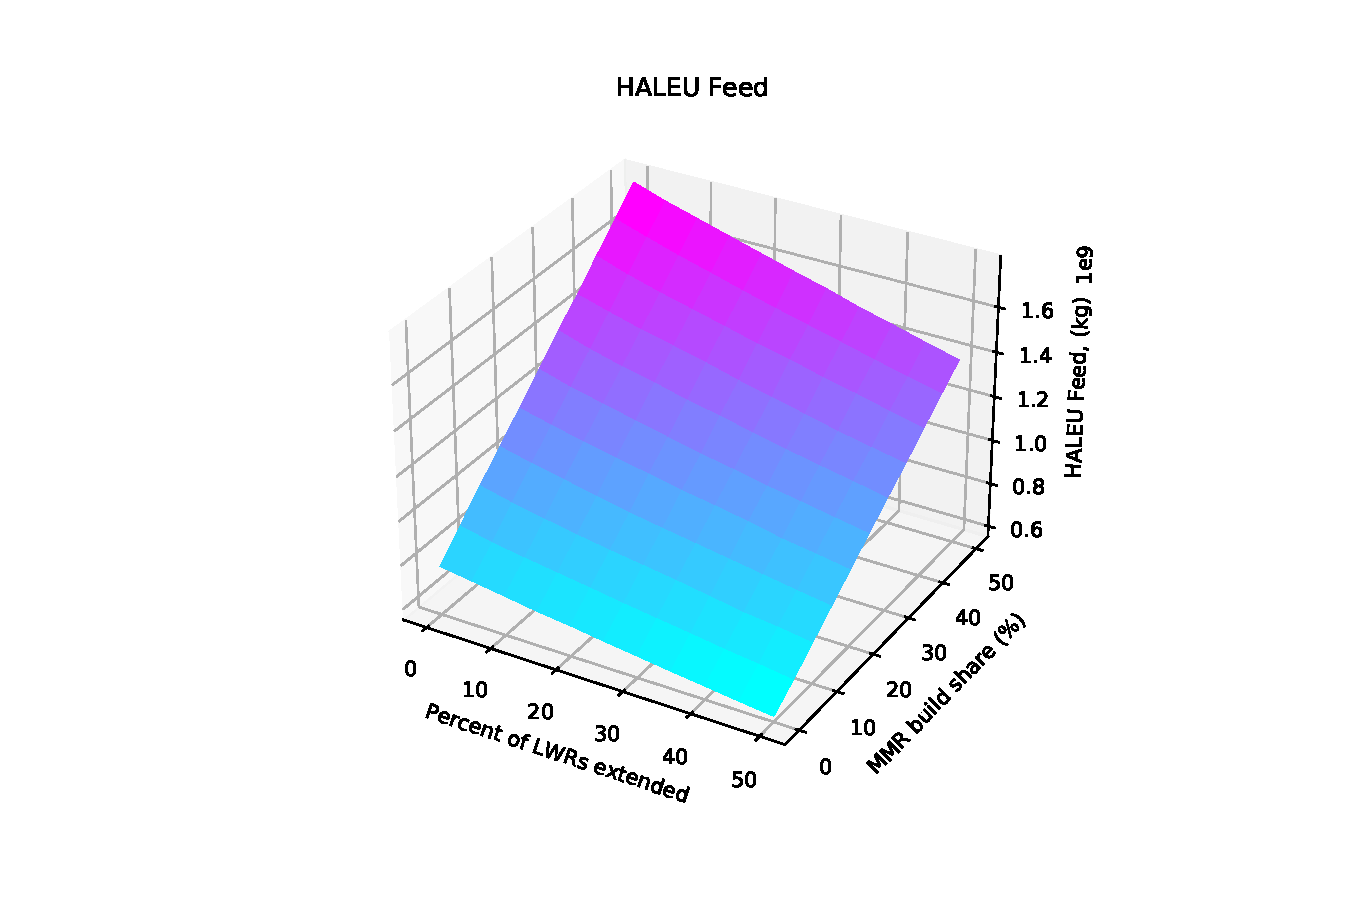
\includegraphics[width=\textwidth, trim=120 0 120 30, clip]{lwr_mmr_share_feed.pdf}
        \caption{Effect on HALEU feed.}
        \label{fig:lwr_mmr_share_feed}
    \end{subfigure}
    \caption{Change in metrics resulting from variations in the 
    LWR lifetimes and MMR build share.}
    \label{fig:lwr_mmr_share}
\end{figure}

\begin{figure}   
    \begin{subfigure}[t]{0.48\textwidth}
        \centering
        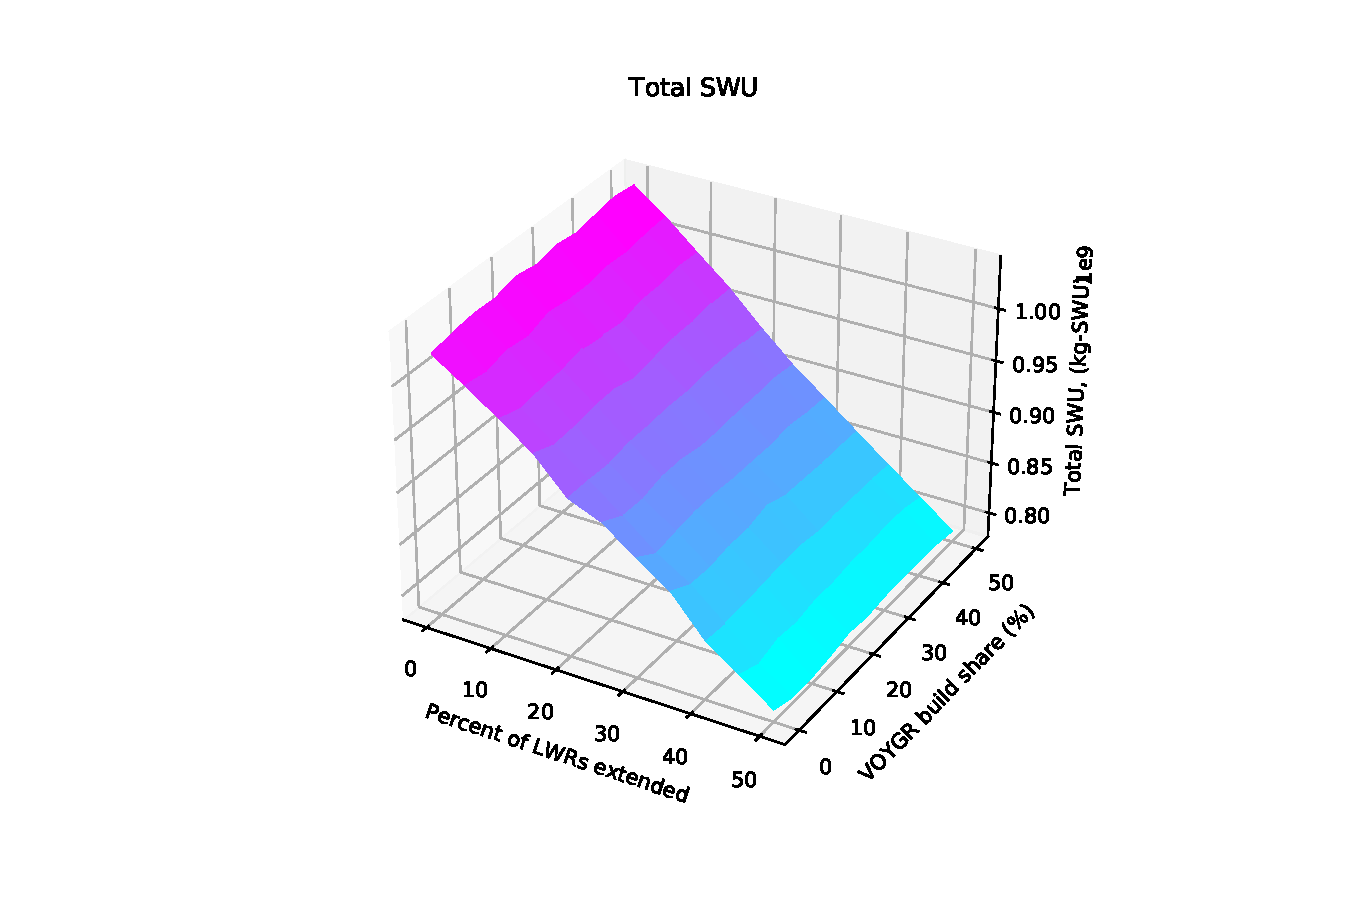
\includegraphics[width=\textwidth, trim=120 0 120 30, clip]{lwr_voygr_share_swu.pdf}
        \caption{Effect on total SWU capacity.}
        \label{fig:lwr_voygr_share_swu}
    \end{subfigure}
    \hfill
    \begin{subfigure}[t]{0.48\textwidth}
        \centering
        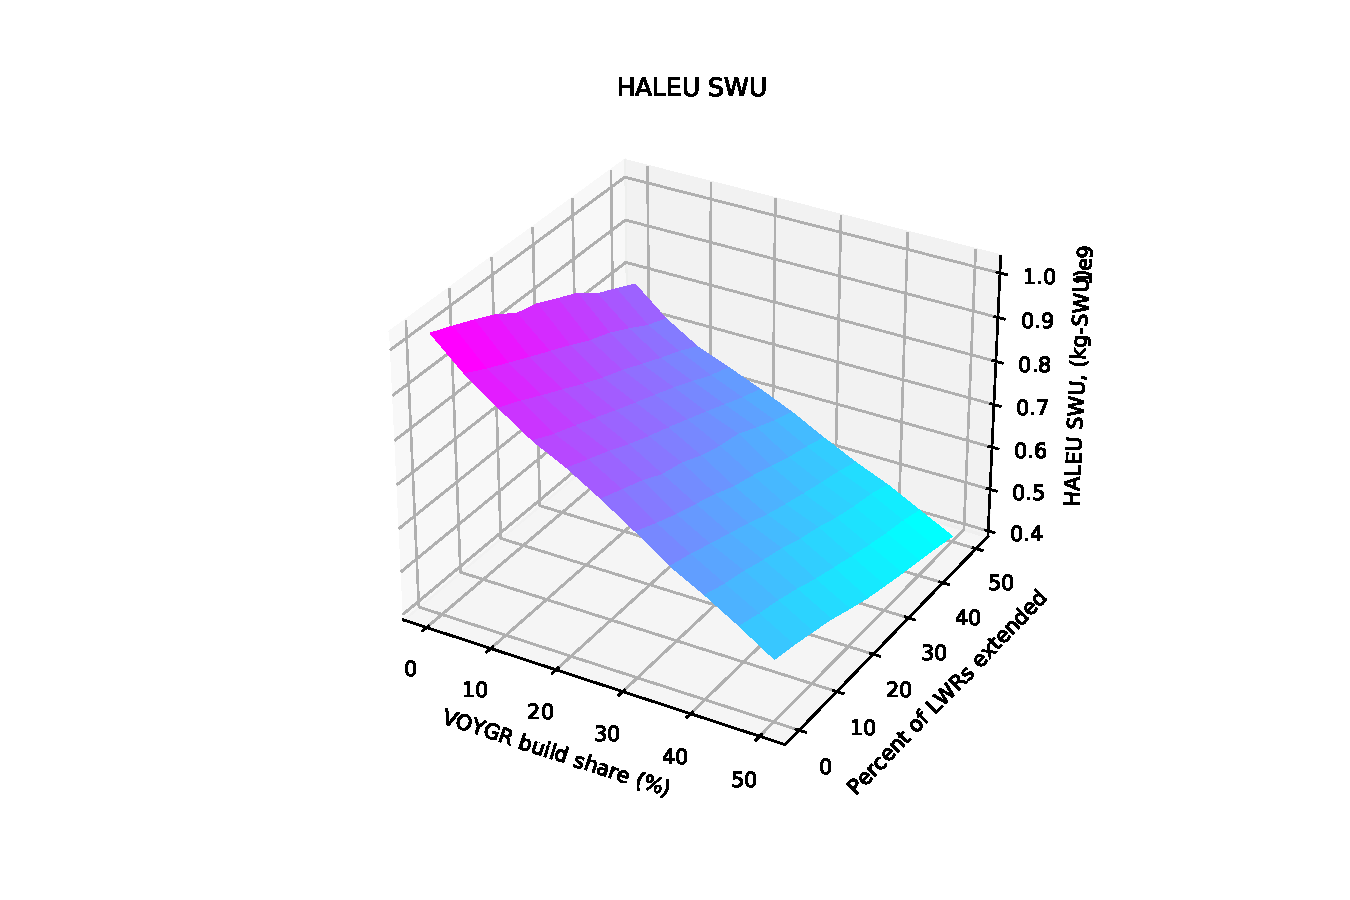
\includegraphics[width=\textwidth, trim=120 0 120 30, clip]{lwr_voygr_share_haleu_swu.pdf}
        \caption{Effect on HALEU SWU capacity.}
        \label{fig:lwr_voygr_share_haleu_swu}
    \end{subfigure}   
    \begin{subfigure}[t]{0.48\textwidth}
        \centering
        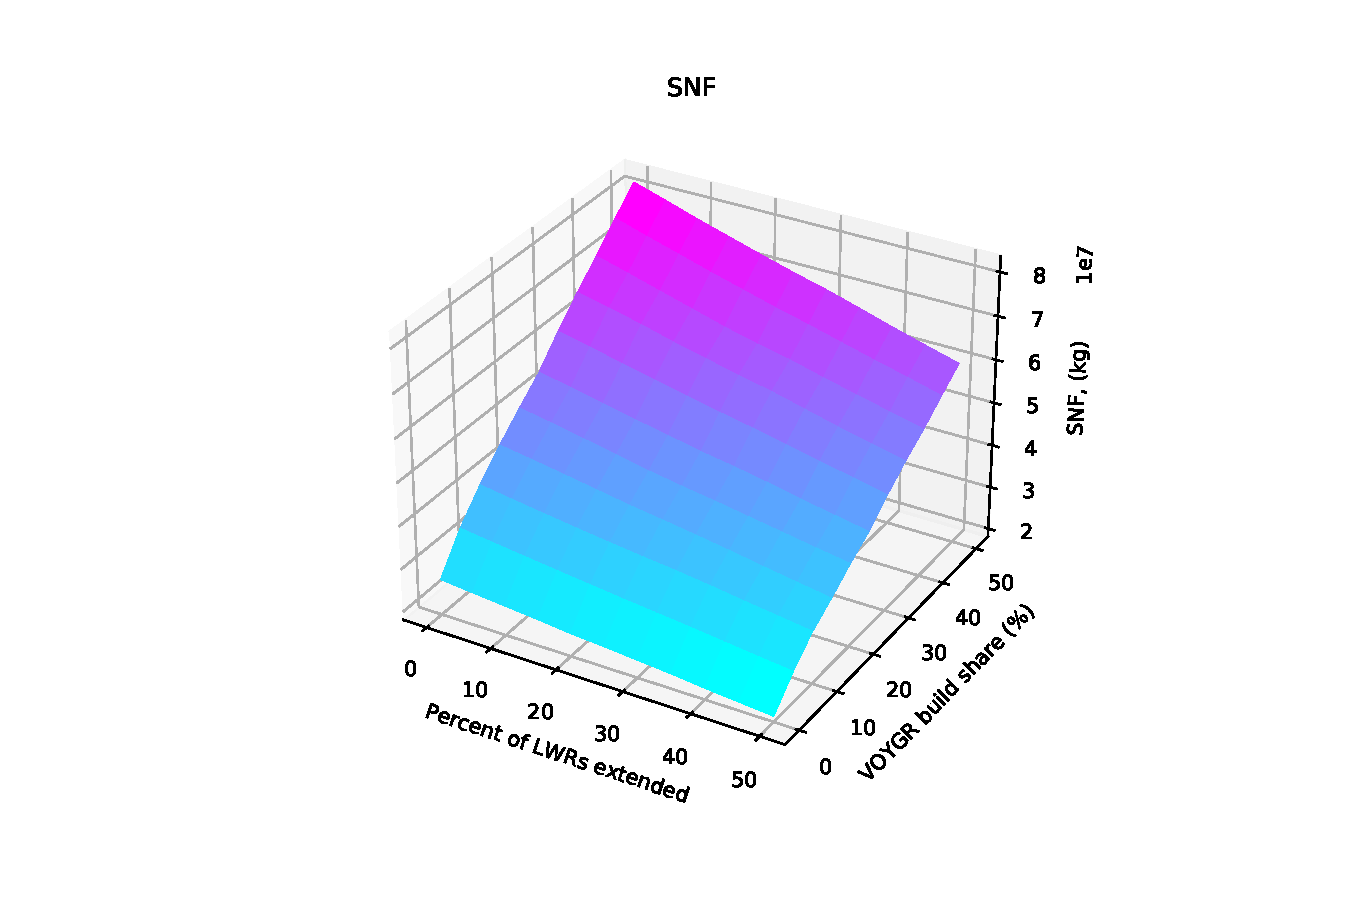
\includegraphics[width=\textwidth, trim=120 0 120 30, clip]{lwr_voygr_share_waste.pdf}
        \caption{Effect on waste mass discharged.}
        \label{fig:lwr_voygr_share_waste}
    \end{subfigure}
    \hfill
    \begin{subfigure}[t]{0.48\textwidth}
        \centering
        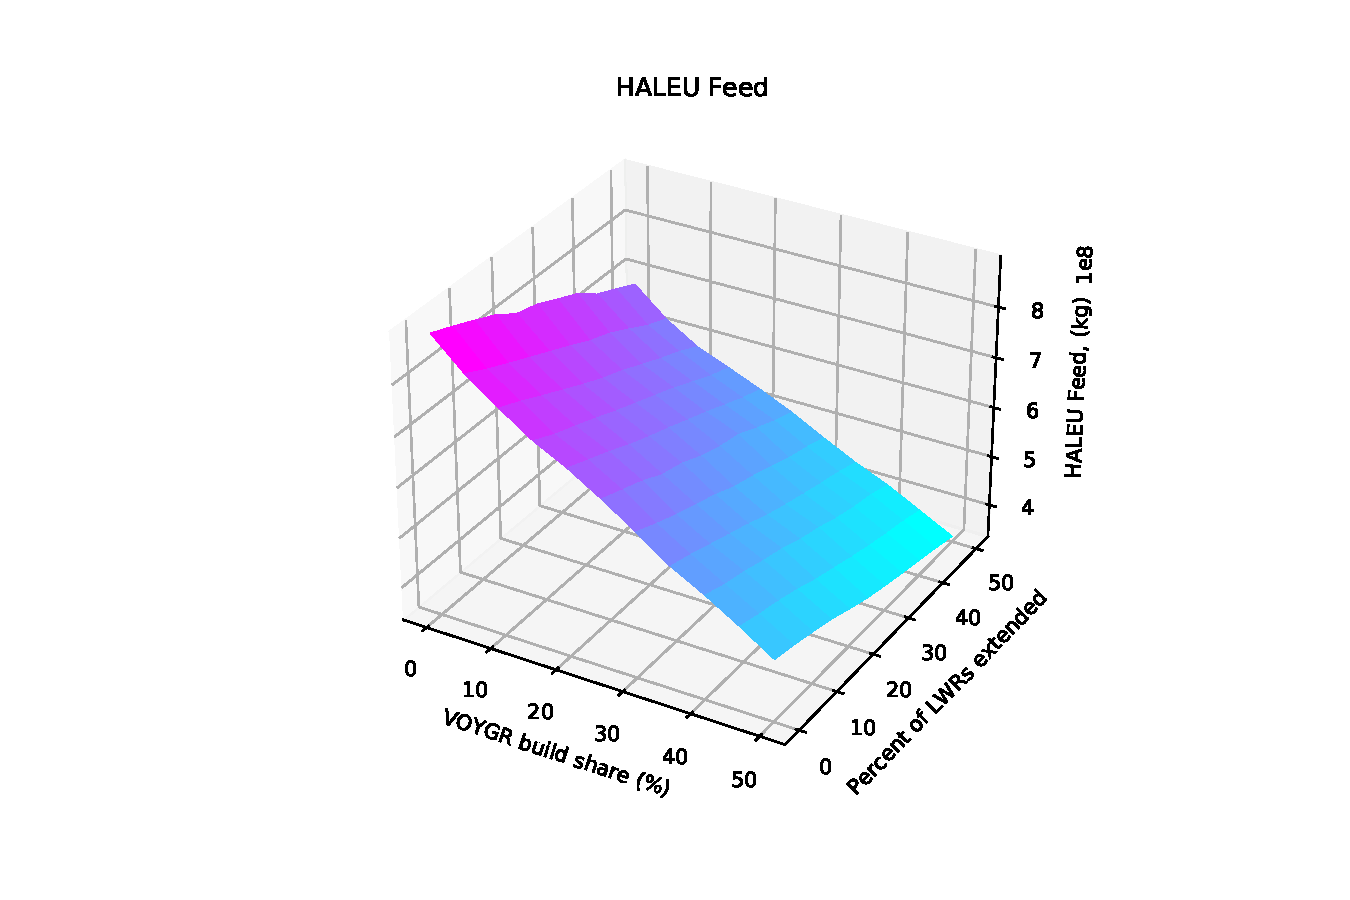
\includegraphics[width=\textwidth, trim=120 0 120 30, clip]{lwr_voygr_share_feed.pdf}
        \caption{Effect on HALEU feed.}
        \label{fig:lwr_voygr_share_feed}
    \end{subfigure}
    \caption{Change in metrics resulting from variations in the 
    LWR lifetimes and VOYGR build share.}
    \label{fig:lwr_voygr_share}
\end{figure}

\begin{figure}
    \begin{subfigure}[t]{0.48\textwidth}
        \centering
        \includegraphics[width=\textwidth, trim=120 0 120 30, clip]{lwr_xe100_burnup_enr_u.pdf}
        \caption{Effect on total fuel mass.}
        \label{fig:lwr_xe100_burnup_enr_u}
    \end{subfigure}
    \hfill
    \begin{subfigure}[t]{0.48\textwidth}
        \centering
        \includegraphics[width=\textwidth, trim=120 0 120 30, clip]{lwr_xe100_burnup_haleu.pdf}
        \caption{Effect on HALEU mass.}
        \label{fig:lwr_xe100_burnup_haleu}
    \end{subfigure}
    
    \begin{subfigure}[t]{0.48\textwidth}
        \centering
        \includegraphics[width=\textwidth, trim=120 0 120 30, clip]{lwr_xe100_burnup_swu.pdf}
        \caption{Effect on total SWU capacity.}
        \label{fig:lwr_xe100_burnup_swu}
    \end{subfigure}
    \hfill
    \begin{subfigure}[t]{0.48\textwidth}
        \centering
        \includegraphics[width=\textwidth, trim=120 0 120 30, clip]{lwr_xe100_burnup_haleu_swu.pdf}
        \caption{Effect on HALEU SWU capacity.}
        \label{fig:lwr_xe100_burnup_haleu_swu}
    \end{subfigure}
\end{figure}

\begin{figure}
    \ContinuedFloat    
    \begin{subfigure}[t]{0.48\textwidth}
        \centering
        \includegraphics[width=\textwidth, trim=120 0 120 30, clip]{lwr_xe100_burnup_waste.pdf}
        \caption{Effect on waste mass discharged.}
        \label{fig:lwr_xe100_burnup_waste}
    \end{subfigure}
    \hfill
    \begin{subfigure}[t]{0.48\textwidth}
        \centering
        \includegraphics[width=\textwidth, trim=120 0 120 30, clip]{lwr_xe100_burnup_feed.pdf}
        \caption{Effect on HALEU feed.}
        \label{fig:lwr_xe100_burnup_feed}
    \end{subfigure}
    \caption{Change in metrics resulting from variations in the 
    LWR lifetimes and the Xe-100 discharge burnup}
    \label{fig:lwr_xe100_burnup}
\end{figure}
\begin{figure}
    \begin{subfigure}[t]{0.48\textwidth}
        \centering
        \includegraphics[width=\textwidth, trim=120 0 120 30, clip]{lwr_mmr_burnup_enr_u.pdf}
        \caption{Effect on total fuel mass.}
        \label{fig:lwr_mmr_burnup__enr_u}
    \end{subfigure}
    \hfill
    \begin{subfigure}[t]{0.48\textwidth}
        \centering
        \includegraphics[width=\textwidth, trim=120 0 120 30, clip]{lwr_mmr_burnup_haleu.pdf}
        \caption{Effect on HALEU mass.}
        \label{fig:lwr_mmr_burnup_haleu}
    \end{subfigure}
\end{figure}

\begin{figure}
    \ContinuedFloat    
    \begin{subfigure}[t]{0.48\textwidth}
        \centering
        \includegraphics[width=\textwidth, trim=120 0 120 30, clip]{lwr_mmr_burnup_swu.pdf}
        \caption{Effect on total SWU capacity.}
        \label{fig:lwr_mmr_burnup_swu}
    \end{subfigure}
    \hfill
    \begin{subfigure}[t]{0.48\textwidth}
        \centering
        \includegraphics[width=\textwidth, trim=120 0 120 30, clip]{lwr_mmr_burnup_haleu_swu.pdf}
        \caption{Effect on HALEU SWU capacity.}
        \label{fig:lwr_mmr_burnup_haleu_swu}
    \end{subfigure}
    
    \begin{subfigure}[t]{0.48\textwidth}
        \centering
        \includegraphics[width=\textwidth, trim=120 0 120 30, clip]{lwr_mmr_burnup_waste.pdf}
        \caption{Effect on waste mass discharged.}
        \label{fig:lwr_mmr_burnup_waste}
    \end{subfigure}
    \hfill
    \begin{subfigure}[t]{0.48\textwidth}
        \centering
        \includegraphics[width=\textwidth, trim=120 0 120 30, clip]{lwr_mmr_burnup_feed.pdf}
        \caption{Effect on HALEU feed.}
        \label{fig:lwr_mmr_burnup_feed}
    \end{subfigure}
    \caption{Change in metrics resulting from variations in the 
    LWR lifetimes and MMR discharge burnup.}
    \label{fig:lwr_mmr_burnup}
\end{figure}

\begin{figure}
    \begin{subfigure}[t]{0.48\textwidth}
        \centering
        \includegraphics[width=\textwidth, trim=120 0 120 30, clip]{mmr_share_xe100_burnup_haleu.pdf}
        \caption{Effect on HALEU mass.}
        \label{fig:mmr_share_xe100_burnup_haleu}
    \end{subfigure}
    \hfill 
    \begin{subfigure}[t]{0.48\textwidth}
        \centering
        \includegraphics[width=\textwidth, trim=120 0 120 30, clip]{mmr_share_xe100_burnup_swu.pdf}
        \caption{Effect on total SWU capacity.}
        \label{fig:mmr_share_xe100_burnup_swu}
    \end{subfigure}
    \hfill
    \begin{subfigure}[t]{0.48\textwidth}
        \centering
        \includegraphics[width=\textwidth, trim=120 0 120 30, clip]{mmr_share_xe100_burnup_haleu_swu.pdf}
        \caption{Effect on HALEU SWU capacity.}
        \label{fig:mmr_share_xe100_burnup_haleu_swu}
    \end{subfigure}
    \hfill
    \begin{subfigure}[t]{0.48\textwidth}
        \centering
        \includegraphics[width=\textwidth, trim=120 0 120 30, clip]{mmr_share_xe100_burnup_waste.pdf}
        \caption{Effect on waste mass discharged.}
        \label{fig:mmr_share_xe100_burnup_waste}
    \end{subfigure}
\end{figure}

\begin{figure}
    \ContinuedFloat
    \begin{subfigure}[t]{0.48\textwidth}
        \centering
        \includegraphics[width=\textwidth, trim=120 0 120 30, clip]{mmr_share_xe100_burnup_feed.pdf}
        \caption{Effect on HALEU feed.}
        \label{fig:mmr_share_xe100_burnup_feed}
    \end{subfigure}
    \caption{Change in metrics resulting from variations in the 
    MMR build share and Xe-100 discharge burnup.}
    \label{fig:mmr_share_xe100_burnup}
\end{figure}

\begin{figure}
    \begin{subfigure}[t]{0.48\textwidth}
        \centering
        \includegraphics[width=\textwidth, trim=120 0 120 30, clip]{mmr_share_mmr_burnup_enr_u.pdf}
        \caption{Effect on total fuel mass.}
        \label{fig:mmr_share_mmr_burnup_enr_u}
    \end{subfigure}
    \hfill
    \begin{subfigure}[t]{0.48\textwidth}
        \centering
        \includegraphics[width=\textwidth, trim=120 0 120 30, clip]{mmr_share_mmr_burnup_haleu.pdf}
        \caption{Effect on HALEU mass.}
        \label{fig:mmr_share_mmr_burnup_haleu}
    \end{subfigure}
\end{figure}

\begin{figure}
    \ContinuedFloat    
    \begin{subfigure}[t]{0.48\textwidth}
        \centering
        \includegraphics[width=\textwidth, trim=120 0 120 30, clip]{mmr_share_mmr_burnup_swu.pdf}
        \caption{Effect on total SWU capacity.}
        \label{fig:mmr_share_mmr_burnup_swu}
    \end{subfigure}
    \hfill
    \begin{subfigure}[t]{0.48\textwidth}
        \centering
        \includegraphics[width=\textwidth, trim=120 0 120 30, clip]{mmr_share_mmr_burnup_haleu_swu.pdf}
        \caption{Effect on HALEU SWU capacity.}
        \label{fig:mmr_share_mmr_burnup_haleu_swu}
    \end{subfigure}
    
    \begin{subfigure}[t]{0.48\textwidth}
        \centering
        \includegraphics[width=\textwidth, trim=120 0 120 30, clip]{mmr_share_mmr_burnup_waste.pdf}
        \caption{Effect on waste mass discharged.}
        \label{fig:mmr_share_mmr_burnup_waste}
    \end{subfigure}
    \hfill
    \begin{subfigure}[t]{0.48\textwidth}
        \centering
        \includegraphics[width=\textwidth, trim=120 0 120 30, clip]{mmr_share_mmr_burnup_feed.pdf}
        \caption{Effect on HALEU feed.}
        \label{fig:mmr_share_mmr_burnup_feed}
    \end{subfigure}
    \caption{Change in metrics resulting from variations in the 
    MMR build share and MMR discharge burnup.}
    \label{fig:mmr_share_mmr_burnup}
\end{figure}

\begin{figure}    
    \begin{subfigure}[t]{0.48\textwidth}
        \centering
        \includegraphics[width=\textwidth, trim=120 0 120 30, clip]{xe100_share_xe100_burnup_swu.pdf}
        \caption{Effect on total SWU capacity.}
        \label{fig:xe100_share_xe100_burnup_swu}
    \end{subfigure}
    \hfill
    \begin{subfigure}[t]{0.48\textwidth}
        \centering
        \includegraphics[width=\textwidth, trim=120 0 120 30, clip]{xe100_share_xe100_burnup_haleu_swu.pdf}
        \caption{Effect on HALEU SWU capacity.}
        \label{fig:xe100_share_xe100_burnup_haleu_swu}
    \end{subfigure}
    
    \begin{subfigure}[t]{0.48\textwidth}
        \centering
        \includegraphics[width=\textwidth, trim=120 0 120 30, clip]{xe100_share_xe100_burnup_waste.pdf}
        \caption{Effect on waste mass discharged.}
        \label{fig:xe100_share_xe100_burnup_waste}
    \end{subfigure}
    \hfill
    \begin{subfigure}[t]{0.48\textwidth}
        \centering
        \includegraphics[width=\textwidth, trim=120 0 120 30, clip]{xe100_share_xe100_burnup_feed.pdf}
        \caption{Effect on HALEU feed.}
        \label{fig:xe100_share_xe100_burnup_feed}
    \end{subfigure}
    \caption{Change in metrics resulting from variations in the 
    Xe-100 build share and Xe-100 discharge burnup.}
    \label{fig:xe100_share_xe100_burnup}
\end{figure}
\begin{figure}
    \begin{subfigure}[t]{0.48\textwidth}
        \centering
        \includegraphics[width=\textwidth, trim=120 0 120 30, clip]{xe100_share_mmr_burnup_enr_u.pdf}
        \caption{Effect on total fuel mass.}
        \label{fig:xe100_share_mmr_burnup_enr_u}
    \end{subfigure}
    \hfill
    \begin{subfigure}[t]{0.48\textwidth}
        \centering
        \includegraphics[width=\textwidth, trim=120 0 120 30, clip]{xe100_share_mmr_burnup_haleu.pdf}
        \caption{Effect on HALEU mass.}
        \label{fig:xe100_share_mmr_burnup_haleu}
    \end{subfigure}
    
    \begin{subfigure}[t]{0.48\textwidth}
        \centering
        \includegraphics[width=\textwidth, trim=120 0 120 30, clip]{xe100_share_mmr_burnup_swu.pdf}
        \caption{Effect on total SWU capacity.}
        \label{fig:xe100_share_mmr_burnup_swu}
    \end{subfigure}
    \hfill
    \begin{subfigure}[t]{0.48\textwidth}
        \centering
        \includegraphics[width=\textwidth, trim=120 0 120 30, clip]{xe100_share_mmr_burnup_haleu_swu.pdf}
        \caption{Effect on HALEU SWU capacity.}
        \label{fig:xe100_share_mmr_burnup_haleu_swu}
    \end{subfigure}    
\end{figure}

\begin{figure}
    \ContinuedFloat    
    \begin{subfigure}[t]{0.48\textwidth}
        \centering
        \includegraphics[width=\textwidth, trim=120 0 120 30, clip]{xe100_share_mmr_burnup_waste.pdf}
        \caption{Effect on waste mass discharged.}
        \label{fig:xe100_share_mmr_burnup_waste}
    \end{subfigure}
    \hfill
    \begin{subfigure}[t]{0.48\textwidth}
        \centering
        \includegraphics[width=\textwidth, trim=120 0 120 30, clip]{xe100_share_mmr_burnup_feed.pdf}
        \caption{Effect on HALEU feed.}
        \label{fig:xe100_share_mmr_burnup_feed}
    \end{subfigure}
    \caption{Change in metrics resulting from variations in the 
    Xe-100 build share and MMR discharge burnup}
    \label{fig:xe100_share_mmr_burnup}
\end{figure}
\begin{figure}
    \begin{subfigure}[t]{0.48\textwidth}
        \centering
        \includegraphics[width=\textwidth, trim=120 0 120 30, clip]{voygr_share_xe100_burnup_enr_u.pdf}
        \caption{Effect on total fuel mass.}
        \label{fig:voygr_share_xe100_burnup_enr_u}
    \end{subfigure}
    \hfill
    \begin{subfigure}[t]{0.48\textwidth}
        \centering
        \includegraphics[width=\textwidth, trim=120 0 120 30, clip]{voygr_share_xe100_burnup_haleu.pdf}
        \caption{Effect on HALEU mass.}
        \label{fig:voygr_share_xe100_burnup_haleu}
    \end{subfigure}
\end{figure}

\begin{figure}
    \ContinuedFloat    
    \begin{subfigure}[t]{0.48\textwidth}
        \centering
        \includegraphics[width=\textwidth, trim=120 0 120 30, clip]{voygr_share_xe100_burnup_swu.pdf}
        \caption{Effect on total SWU capacity.}
        \label{fig:voygr_share_xe100_burnup_swu}
    \end{subfigure}
    \hfill
    \begin{subfigure}[t]{0.48\textwidth}
        \centering
        \includegraphics[width=\textwidth, trim=120 0 120 30, clip]{voygr_share_xe100_burnup_haleu_swu.pdf}
        \caption{Effect on HALEU SWU capacity.}
        \label{fig:voygr_share_xe100_burnup_haleu_swu}
    \end{subfigure}
    
    \begin{subfigure}[t]{0.48\textwidth}
        \centering
        \includegraphics[width=\textwidth, trim=120 0 120 30, clip]{voygr_share_xe100_burnup_waste.pdf}
        \caption{Effect on waste mass discharged.}
        \label{fig:voygr_share_xe100_burnup_waste}
    \end{subfigure}
    \hfill
    \begin{subfigure}[t]{0.48\textwidth}
        \centering
        \includegraphics[width=\textwidth, trim=120 0 120 30, clip]{voygr_share_xe100_burnup_feed.pdf}
        \caption{Effect on HALEU feed.}
        \label{fig:voygr_share_xe100_burnup_feed}
    \end{subfigure}
    \caption{Change in metrics resulting from variations in the 
    VOYGR build share and Xe-100 discharge burnup.}
    \label{fig:voygr_share_xe100_burnup}
\end{figure}
\begin{figure}
    \begin{subfigure}[t]{0.48\textwidth}
        \centering
        \includegraphics[width=\textwidth, trim=120 0 120 30, clip]{voygr_share_mmr_burnup_enr_u.pdf}
        \caption{Effect on total fuel mass.}
        \label{fig:voygr_share_mmr_burnupenr_u}
    \end{subfigure}
    \hfill
    \begin{subfigure}[t]{0.48\textwidth}
        \centering
        \includegraphics[width=\textwidth, trim=120 0 120 30, clip]{voygr_share_mmr_burnup_haleu.pdf}
        \caption{Effect on HALEU mass.}
        \label{fig:voygr_share_mmr_burnup_haleu}
    \end{subfigure}
    
    \begin{subfigure}[t]{0.48\textwidth}
        \centering
        \includegraphics[width=\textwidth, trim=120 0 120 30, clip]{voygr_share_mmr_burnup_swu.pdf}
        \caption{Effect on total SWU capacity.}
        \label{fig:voygr_share_mmr_burnup_swu}
    \end{subfigure}
    \hfill
    \begin{subfigure}[t]{0.48\textwidth}
        \centering
        \includegraphics[width=\textwidth, trim=120 0 120 30, clip]{voygr_share_mmr_burnup_haleu_swu.pdf}
        \caption{Effect on HALEU SWU capacity.}
        \label{fig:voygr_share_mmr_burnup_haleu_swu}
    \end{subfigure}
\end{figure}

\begin{figure}
    \ContinuedFloat    
    \begin{subfigure}[t]{0.48\textwidth}
        \centering
        \includegraphics[width=\textwidth, trim=120 0 120 30, clip]{voygr_share_mmr_burnup_waste.pdf}
        \caption{Effect on waste mass discharged.}
        \label{fig:voygr_share_mmr_burnup_waste}
    \end{subfigure}
    \hfill
    \begin{subfigure}[t]{0.48\textwidth}
        \centering
        \includegraphics[width=\textwidth, trim=120 0 120 30, clip]{voygr_share_mmr_burnup_feed.pdf}
        \caption{Effect on HALEU feed.}
        \label{fig:voygr_share_mmr_burnup_feed}
    \end{subfigure}
    \caption{Change in metrics resulting from variations in the 
    VOYGR build share and MMR discharge burnup.}
    \label{fig:voygr_share_mmr_burnup}
\end{figure}